\documentclass{article}
\usepackage[utf8]{inputenc}
\usepackage{listings}
% \usepackage{xcolor}
\usepackage[table]{xcolor}
\usepackage{amsmath} 
\usepackage{cancel}
\usepackage{fancyhdr}
\usepackage{xfrac}
\usepackage{amssymb}
\usepackage{subfig}
\usepackage{graphicx}
\usepackage{wrapfig}
\usepackage{minted}
\usepackage{tikz}
\usepackage{pgfplots}
\usepackage{hyperref}
% fissa le footnotes in fondo alla pagina
\usepackage[bottom]{footmisc}
\usetikzlibrary{decorations.pathreplacing,calligraphy}

% FIX MARGINI
\usepackage{geometry}
\geometry{
a4paper,
total={170mm, 257mm},
left=20mm,
top=20mm,
}

% COMANDI CUSTOM
% \abovemargin{1pt} imposta il margine sopra una equazione \[ \] a 1 pt
\newcommand{\abovemargin}[1]{\setlength\abovedisplayskip{#1}}
% \s = \sigma
\newcommand{\s}{\sigma}
% \sumi = {\sum}_i
\newcommand{\sumi}{{\sum}_i}

% \uloosdot{parola} = parola sottolineata con lineette (utile per le footnotes)
\newcommand{\uloosdash}[1]{%
    \tikz[baseline=(todotted.base)]{
        \node[inner sep=1pt,outer sep=0pt] (todotted) {#1};
        \draw[loosely dashed] (todotted.south west) -- (todotted.south east);
    }%
}%

% DEFINIZIONE DEGLI SNIPPET DI CODICE
\definecolor{codegreen}{rgb}{0,0.6,0}
\definecolor{codegray}{rgb}{0.5,0.5,0.5}
\definecolor{codepurple}{rgb}{0.58,0,0.82}
\definecolor{backcolour}{rgb}{0.95,0.95,0.92}
\lstdefinestyle{style}{
    backgroundcolor=\color{backcolour},   
    commentstyle=\color{codegreen},
    keywordstyle=\color{magenta},
    numberstyle=\tiny\color{codegray},
    stringstyle=\color{codepurple},
    basicstyle=\ttfamily\footnotesize,
    breakatwhitespace=false,         
    breaklines=true,                 
    captionpos=b,                    
    keepspaces=true,                 
    numbers=left,                    
    numbersep=5pt,                  
    showspaces=false,                
    showstringspaces=false,
    showtabs=false,                  
    tabsize=2
}
\lstset{style=style}

% DEFINIZIONE COLORI
\definecolor{lightgreen}{rgb}{0.5,1,0.5}
\definecolor{lightred}{rgb}{1,0.5,0.5}
\definecolor{Orange}{HTML}{F58137}
\definecolor{ForestGreen}{HTML}{009B55}

\renewcommand{\figurename}{Figura}
\newcommand{\red}[1]{\color{red}{#1}\normalcolor}
\newcommand{\orange}[1]{\color{Orange}{#1}\normalcolor}
\newcommand{\green}[1]{\color{ForestGreen}{#1}\normalcolor}
\usepgfplotslibrary{fillbetween}
\usetikzlibrary{positioning}
\usetikzlibrary{shapes.geometric}
\usepackage{mdframed}
\usepackage{amsthm}
\usepackage{mathtools}
\usepackage{framed}
\usetikzlibrary{patterns}
\usepackage{pdflscape}
\usepackage{rotating}
\usepackage{makecell}
\usepackage{pgfplots}

% Aggiunti MANGIO
\usepackage{multirow}
\usepackage{tabularx}

\usepackage[yyyymmdd]{datetime}
\renewcommand{\dateseparator}{-}

% TEOREMI
\newtheorem*{teorema}{Teorema}
\newtheorem*{corollario}{Corollario}
\newtheorem*{dimostrazione}{Dimostrazione}
\newtheorem{proprieta}{Proprietà}
\newtheorem*{esempio}{Esempio}

\newcommand{\E}{\mathbb{E}}

\title{
Statistica e analisi dei dati \\
\small{Appunti completi e \textit{meravigliosi}, in \LaTeX}
}
\author{Mattia Oldani, Marco Aceti, Daniele Ceribelli}
\date{}
\pgfplotsset{compat=1.18}

% note 
\pagestyle{fancy}
\fancyhf{}
\lhead{Statistica e analisi dei dati}
\rhead{\rightmark}
\lfoot{\thepage}

% INIZIO DEL DOCUMENTO
\begin{document}

% CREAZIONE TITOLO E AUTORE
\maketitle

% DEFINIZIONE INDICE
\renewcommand*\contentsname{Indice}
\tableofcontents



% INIZIO EFFETTIVO DELLE NOTE
\newpage

% Statistica descrittiva
\section{Statistica descrittiva}
La \textbf{statistica} è una disciplina che permette di trarre delle conclusioni partendo da dati in situazioni di incertezza; in particolare, la \textbf{statistica descrittiva} si occupa dei metodi di esposizione e sintesi dei dati.

\subsection{Concetti preliminari}
La \textbf{popolazione} è l'insieme degli elementi (individui) da cui si vorrebbero acquisire i dati; spesso, per questioni di praticità, non è però sempre possibile eseguire la raccolta dati su tutta la popolazione. 
\newline
\noindent Un \textbf{campione} è un \textit{sottoinsieme rappresentativo} della popolazione su cui si fanno le analisi.
Un buon campione deve essere casuale (evitando il \textbf{sotto-campionamento} di sottoinsiemi della popolazione) e la scelta di un individuo non deve influenzare la scelta dei successivi.
Per fare in modo che il campione sia casuale si sfrutta il \textbf{campionamento casuale}, ovvero ogni elemento deve avere la stessa probabilità di essere estratto (in seguito si capirà meglio il significato di probabilità), questo garantisce che il campione sia rappresentativo dell'intera popolazione.

\noindent Quando la popolazione è divisa in \textit{sottoinsiemi non omogenei} può essere complicato ottenere un campione casuale. Per ovviare a ciò si utilizza la tecnica del \textbf{campione casuale stratificato}: in base alla \textbf{frequenza relativa} di ogni sottoinsieme si sceglie un certo numero di elementi di esso da inserire nel campione; in sostanza, gli elementi del campione si pesano in base alla frequenza relativa.

\noindent Ultimi concetti importanti sono le \textbf{frequenze}: 
\begin{itemize}
    \item \textbf{$f_j$ assoluta}: numero di volte che un dato compare in un campione;
    \item \textbf{$f'_j$ relativa}: frazione di volte che un dato compare nel campione. Si calcola con 
    \setlength\abovedisplayskip{3pt} \[
        f'_j = \frac{f_j}{n}.
    \]
\end{itemize}

\subsection{Tipi di dati}
Introduciamo ora le differenze tra i tre tipi di dati raggruppandoli in gruppi: 
\begin{itemize}
    \item si parla di dati \textbf{quantitativi} se l’esito della misurazione è una quantità numerica;
    \item si parla invece di dati \textbf{qualitativi} (o categorici, o nominali) quando la misurazione è fatta scegliendo un’etichetta a partire da un insieme tra quelli disponibili.
\end{itemize}

\subsubsection{Classificazione dati quantitativi}
Per quanto riguarda i dati quantitativi, viene spesso fatto riferimento alla differenza tra dati \textbf{discreti} e \textbf{continui} in funzione del tipo di insieme di valori che questi possono assumere. Possiamo quindi, a livello teorico, distinguere un insieme di dati discreti se i valori assunti sono solo interi e quindi non ci sono valori all'interno di un intervallo (per esempio il numero di tentativi non ha senso classificarlo come continuo siccome non esiste il valore $3.5$), mentre nel continuo ci saranno infiniti valori tra un numero intero e un altro (come per esempio la percentuale).

\subsubsection{Classificazione dati qualitativi}
I dati qualitativi vengono spesso ulteriormente classificati come binari, nominali oppure
ordinali. Si parla di dati \textbf{binari} quando l’osservazione può avere solo due esiti tra loro
non confrontabili. Anche nei dati \textbf{nominali}, i valori osservabili non sono tra loro confrontabili, sebbene non vi sia limite sul numero di diverse etichette.  Detto in altri termini, in questo tipo di dati è solo possibile stabilire una relazione di equivalenza tra i valori osservabili. Nei dati \textbf{ordinali}, invece, è possibile stabilire una relazione d’ordine tra i valori osservabili, sarà quindi possibile distinguere tra due dati diversi quale sia il più piccolo e quale sia il più grande.

% chap 11.6 RS

\subsection{Funzione cumulativa empirica}
La \textbf{funzione cumulativa empirica}, (\textbf{ECDF}), è una funzione di variabile reale che rappresenta la funzione di ripartizione della misura empirica di un campione. Dato un insieme di osservazioni $\{x_1, \, ..., \, x_n\}$ è definita come quella funzione $\hat{F}: \mathbb R \rightarrow [0, 1]$ tale che per ogni $x \in \mathbb R$ assume un valore pari alla frequenza relativa delle osservazioni che risultano essere minori o uguali a $x$.
$$
\hat{F}(x) = \dfrac{\# \{x_i \leq x\}}{n} = \dfrac{1}{n} \sum_{i = 1}^n I_{(- \infty, x]}(x_i)
$$
Siccome possiamo vedere questa funzione come una stima della funzione di ripartizione, allora questa sarà un buon stimatore e consistente in media quadratica per la funzione di ripartizione.

\subsection{Indici di centralità}
Con gli \textbf{indici di centralità} si possono dare delle informazioni sulla \textit{``grandezza"} dei dati nel campione e descrivere attorno a quale valore si forma la rosa dei valori.
Per tutti gli indici si utilizza $n$ per indicare la \textbf{dimensione} (o \textbf{taglia}) del campione e $\{x_1, \, \dots, \, x_n\}$ il campione stesso.

\subsubsection{Media campionaria}
\begin{flushleft}
La \textbf{media campionaria}\footnote{Con il termine \textit{campionaria} si intende che i dati di cui si sta facendo la media fanno parte di un campione rappresentativo di una popolazione più ampia (quindi ci si riferisce alla statistica e non alla probabilità)} è la media aritmetica degli elementi del campione. 
Si indica con $\overline x$ e si definisce con $$
\boxed{
    \overline{x} = \frac{1}{n}\sumi{x_i}
}.
$$

La media si comporta bene con la \textbf{traslazione} e la \textbf{scalatura} dei dati: sia $X = \{x_1, \, x_2, \, \dots, \, x_n\}$ un campione di $n$ elementi con media campionaria $\overline x$, assumiamo di voler definire dal precedente un nuovo campione $Y = \{ y_1, \, y_2, \, \dots, \, y_n \}$ con media campionaria $\overline y$. 
\newline 
Se definiamo gli elementi di $Y$ come una \textit{traslazione} ($+ \, b$) degli elementi di $X$, osserviamo che $\overline y = \overline x + b$.
\[
\forall_i \ 
y_i = x_i + b \Rightarrow \overline{y} = \frac{1}{n}\sum\limits_{i=1}^{n}{y_i} = \frac{1}{n}\sum\limits_{i=1}^{n}{x_i} + \frac{1}{n}\sum\limits_{i=1}^{n}{b} = \overline{x} + \frac{b \cdot \cancel{n}}{\cancel{n}} = \overline{x} + b.
\]

Se invece definiamo gli elementi di $Y$ come una \textit{scalatura} ($\cdot \, a$) degli elementi di $X$, osserviamo che $\overline y = a \overline x$.

%% fix margine
\setlength\abovedisplayskip{1pt}

$$
\forall_i \ y_i = ax_i \Rightarrow \overline{y} = \frac{1}{n}\sum\limits_{i=1}^{n}{y_i} = \frac{a}{n}\sum\limits_{i=1}^{n}{x_i} = a\overline{x}.
$$


Possiamo quindi concludere che 
\[
\boxed{
    \forall_i \ y_i = ax_i + b \Rightarrow 
    \overline{y} = a\overline{x} + b
} .
\]
\end{flushleft} 
La media campionaria è quindi un \textbf{operatore lineare} ma \textbf{non è uno stimatore robusto} rispetto agli \textit{outlier}, ovvero valori molto più grandi o molto più piccoli della media che possono falsare notevolmente le conclusioni. \\
Le differenze tra ciascun valore dei dati e la media campionaria si chiamano \textbf{scarti}, inoltre la somma di tutti gli scarti vale sempre $0$.
\newline \newline
Esistono altri due modi per calcolare la media campionaria:
\begin{itemize}
    \item \textbf{tabella delle frequenze assolute}: è una tabella che contiene, per ogni valore $x$ del campione, la frequenza assoluta di $x$ all'interno del campione. 
    Per calcolare la media si sommano i prodotti tra il valore e la frequenza associata e si divide per la somma delle frequenze.
    Siano $(x_j, \, f_j)$ le coppie presenti nella tabella e $k$ il numero di elementi, allora
    \setlength\abovedisplayskip{2pt} \[
    \overline{x} =
    \dfrac{
        \sum\limits_{j=1}^{k}{x_j f_j}
    }{
        \sum\limits_{j=1}^{k}{f_j}
    }.
    \]
    La formula precedente riesce a calcolare la media anche se gli elementi del campione non sono descritti in maniera estensiva.
    
    \item \textbf{tabella delle frequenze relative}: è una tabella che contiene, per ogni valore del campione, la frequenza relativa nel campione stesso. A differenza del caso precedente, la sommatoria riguarda solo il prodotto tra il dato e la sua frequenza relativa. Siano quindi $(x_j, \, f'_j)$ le coppie presenti nella tabella e $k$ il numero di elementi, allora
    \[
    \overline{x} = \sum\limits_{j=1}^{k}{x_j f'_j}.
    \]
\end{itemize}

\noindent L'operazione di \textbf{normalizzazione delle frequenze} consiste nel dividere ciascuna frequenza per la somma totale delle frequenze per assicurare che la somma delle frequenze normalizzate sia uguale a $1$ e che le frequenze rappresentino ora le proporzioni o le probabilità relative delle categorie o degli eventi.
\noindent La media campionaria \textbf{non è applicabile} nel caso in cui si stiano trattando \textit{dati non quantitativi}

\subsubsection{Mediana campionaria}
La \textbf{mediana campionaria} è un'altra proprietà di un campione.
Per ottenere la mediana, bisogna prima ordinare il campione e successivamente considerare il valore centrale (nel caso di campioni di taglia pari, si considera la media aritmetica dei due valori centrali).
\newline
\noindent La mediana \textbf{è uno stimatore molto robusto} perché considera sempre i valori centrali, a prescindere dalle operazioni di traslazione o scalatura che vengono applicate a eventuali  \textit{outlier}.
\newline
\noindent Questo indice di centralità soffre il fatto che non è possibile sfruttarlo nel caso in cui i dati del campione \textbf{non siano ordinabili}.

\subsubsection{Moda campionaria}
La \textbf{moda campionaria} di un campione è il valore che compare con frequenza maggiore e per questo può essere utilizzato con qualunque tipo di dato.

\subsubsection{Utilizzo degli indici di centralità}

\begin{center}
\begin{tabular}{ | m{3.5cm} | c | c | c | } 
    \hline &
     %\multicolumn{1}{c}{Media} &
     Media & Mediana & Moda \\
     %\multicolumn{1}{c}{Mediana} & 
     %\multicolumn{1}{c}{Moda} \\
    \hline
    Scalari & 
        \cellcolor{lightgreen} \hspace{0.5cm} Sì \hspace{0.5cm} & 
        \cellcolor{lightgreen} \hspace{0.5cm} Sì \hspace{0.5cm} & 
        \cellcolor{lightgreen} \hspace{0.5cm} Sì \hspace{0.5cm}
    \\ \hline
    Categorie ordinali & 
        \cellcolor{lightred}   \hspace{0.5cm} No \hspace{0.5cm} &  %???????????????
        \cellcolor{lightgreen} \hspace{0.5cm} Sì \hspace{0.5cm} & 
        \cellcolor{lightgreen} \hspace{0.5cm} Sì \hspace{0.5cm}
    \\ \hline
    Categorie non ordinali &
        \cellcolor{lightred}   \hspace{0.5cm} No \hspace{0.5cm} & 
        \cellcolor{lightred}   \hspace{0.5cm} No \hspace{0.5cm} & 
        \cellcolor{lightgreen} \hspace{0.5cm} Sì \hspace{0.5cm} 
    \\ \hline
\end{tabular}
\end{center}

Una peculiarità importante da considerare è quella data dal fatto che se un grafico è simmetrico (ad esempio un istogramma) allora \textbf{media}, \textbf{moda} e \textbf{mediana} campionaria sono approssimativamente vicine.

\subsection{Indici di dispersione}
Due campioni possono avere una media e una mediana campionaria molto simile (medesima centralità), ma essere molto diversi per quanto riguarda il \textit{range} di valori che assumono. Può essere quindi utile introdurre degli indici che misurino la \textbf{dispersione} e la \textbf{variabilità del campione}.
La \textbf{dispersione} misura quanto i valori di una distribuzione  distano da un valore centrale preso come riferimento. 

\subsubsection{Varianza campionaria}
La \textbf{varianza campionaria} misura la distanza che c'è tra ogni punto del campione e la media campionaria.

\paragraph{Calcolo della varianza}
Possiamo tentare di calcolare la varianza sommando per ogni elemento lo scarto tra l'elemento stesso e la media campionaria:
$$
{\sum}_i (x_i - \overline{x}) = 
{\sum}_i x_i - {\sum}_i \overline{x} = 
{\sum}_i x_i - n\overline{x} = 
\cancel{{\sum}_i x_i} - \cancel{{\sum}_i x_i} = 0
$$
\noindent Risultando sempre $0$ questo metodo di calcolo non fornisce nessuna informazione.

\noindent Possiamo quindi provare a calcolare il \textrm{valore assoluto} degli scarti, garantendo una somma $\geq 0$ sempre significativa: se tutti i valori del campione sono uguali la varianza calcolata con questa modalità sarà quindi 0:
\[
{\sum}_i{| x_i - \overline{x} |} = \begin{cases}
> 0 & \text{la varianza dei valori} \\
= 0 & \text{tutti i valori sono uguali} \\
< 0 & \perp
\end{cases}.
\]
\newline
La soluzione ``regge" ma gestire un valore assoluto è spesso scomodo, soprattutto quando si incontrano dei valori negativi. Un altro metodo per garantire valori sempre positivi è \textbf{elevare al quadrato} ogni scarto. Dividiamo successivamente il risultato della sommatoria per $n-1$:
\[
\boxed{
\mathnormal{s}^2 = \frac{1}{n-1} {\sum}_i{(x_i - \overline{x})^2}
}.
\]

\noindent Partendo dalla formula precedente, esiste un altro modo per calcolare la varianza campionaria:
\begin{gather*}
\mathnormal{s}^2 = \frac{1}{n-1}
{\sum}_i{(x_i - \overline{x})^2} = \frac{1}{n-1}{\sum}_i{(x_i^2 - 2x_i\overline{x} + \overline{x}^2)} = \\
\frac{1}{n-1} \biggl ({\sum}_i{x_i^2} -
2\overline{x} \underbrace{{\sum}_i x_i}_{=n\overline x} +
\underbrace{{\sum}_i{\overline{x}^2}} _{=n\overline x^2} \biggr) =
\frac{1}{n-1} \biggl ({\sum}_i{x_i^2} -
2n\overline{x}^2 +
n\overline{x}^2 \biggr ) =
\frac{1}{n-1} \biggl ({\sum}_i{x_i^2} - n\overline{x}^2 \biggr ).
\end{gather*}

\paragraph{Traslazione e scalatura} A differenza della media campionaria, la varianza campionaria \textbf{non è un operatore lineare}. Infatti, non supporta le seguenti proprietà:
\begin{itemize}
    \item \textit{traslazione}: definendo $\forall_i \ y_i = x_i + b$, la varianza non cambia linearmente: $\sigma^2_y \neq \sigma^2_x + b$. Dimostrazione: 
    \[
    \mathnormal{s}^2_y = \frac{1}{n - 1}{\sum}_i{(y_i - \overline{y})^2} = \frac{1}{n - 1}{\sum}_i{(x_i + \cancel b - \overline{x} - \cancel b)^2} = \frac{1}{n - 1}{\sum}_i{(x_i - \overline{x})^2} = \mathnormal{s}_x^2.
    \]
    Ha senso che il termine $b$ si perda: la varianza definisce quanto scarto c'è tra i dati e l'operazione di traslazione cambia solo la loro posizione, non la dispersione.
    \item \textit{scalatura}: ancora, definendo $\forall_i \ y_i = a x_i$ la varianza non cambia linearmente: $\s^2_y \neq a \s^2_x$. Dimostrazione:
    \[ 
    \mathnormal{s}^2_y = \frac{1}{n - 1}\sumi{(y_i - \overline{y})^2} = \frac{1}{n - 1}\sumi{(a x_i - a\overline{x})^2} = \frac{1}{n - 1}\sumi{a^2(x_i - \overline{x})^2} = \frac{a^2}{n - 1}\sumi{(x_i - \overline{x})} = a^2\mathnormal{s}^2_x.
    \]
\end{itemize}

\subsubsection{Deviazione campionaria standard}
La \textbf{deviazione campionaria standard} o \textbf{deviazione standard} si ricava dalla varianza campionaria estraendo la radice quadrata da quest'ultima:
\[
\boxed{
    \mathnormal{s} = \sqrt{\mathnormal{s}^2}} = \sqrt{ \frac{1}{n-1}
    \sumi{(x_i - \overline{x})^2}}
\]

\noindent Anche la deviazione campionaria standard, derivando dalla varianza, \textbf{non è un operatore lineare}. Infatti:
\begin{itemize}
    \item \textit{traslazione}: $\forall_i \ y_i = x_i + b \Rightarrow \mathnormal{s}^2_y = \mathnormal{s}^2_x \Rightarrow \mathnormal{s}_y = \mathnormal{s}_x \neq \mathnormal{s}_x + b$;
    \item \textit{scalatura\footnote{Attenzione, si ricordi che $(\sqrt a)^2 = (a^\frac{1}{2})^2 = a^{\frac{1}{2}\cdot2} = a^{2\cdot\frac{1}{2}} = (\sqrt a^2) = |a| \neq a$.}}: $\forall_i \ y_i = a x_i \Rightarrow \mathnormal{s}^2_y = a^2 \mathnormal{s}^2_x \Rightarrow \mathnormal{s}_y = |a| \mathnormal{s}_x \neq a \mathnormal{s}_x$;
\end{itemize}

\noindent L'operatore radice quadrata è un operatore monotono, quindi nel caso in cui la varianza assuma un valore grande/piccolo allora anche la deviazione standard assumerà un valore grande/piccolo.
Un'altra caratteristica importante è che la deviazione standard possiede la stessa unità di misura dei dati sperimentali, quindi facilita la comprensione della dispersione dei dati rispetto alla media.

\subsubsection{Quantili}
Tentiamo di definire il concetto di quantile partendo da quello di mediana campionaria. La mediana campionaria è il \underline{valore del campione}\footnote{
In caso di campione con numero di elementi pari può capitare che la mediana o il quantile non siano un valore del campione ma la media aritmetica dei due valori centrali. Nel caso particolare dei quantili, si dimostra che se $nq$ è intero allora esistono sempre due quantili ed è quindi necessario calcolare la media aritmetica.
} contemporaneamente maggiore o uguale di almeno la metà degli elementi e minore o uguale dell'altra metà degli elementi.
Possiamo generalizzare il concetto precedente di mediana introducendo il \textbf{quantile}: il quantile di grado $q \in [0,1]$ di un campione di taglia $n$ è il \underline{valore del campione} che è $\ge$ di almeno $nq$ osservazioni e $\le$ di almeno $n(1-q)$ osservazioni.

\noindent Osserviamo che $q$ è un numero reale $\mathbb R$ e può assumere infiniti valori, consentendoci un livello di granularità infinito. Spesso nella pratica, però, non è necessario considerare tutti i valori di $q$, anche perché la taglia del campione è sempre finita. Si possono quindi definire dei quantili particolari che ridefiniscono il \textbf{livello di granularità}:
\begin{itemize}
    \item \textbf{percentili}: il livello è descritto da una percentuale, frazione di 100;
    \item \textbf{decili}: il livello è descritto da una frazione di $10$;
    \item \textbf{quartili}: il livello è descritto da una frazione di $4$.
\end{itemize}

\paragraph{Quartili}
I quartili sono molto interessanti, perché permettono una rappresentazione grafica tramite \textbf{box plot}:

\begin{center}
\begin{tikzpicture}

\draw (-1,0) rectangle (3,1); % box

% frecce + label
\draw[<-] (-1, -0.1) -- (-1, -0.4) node[anchor=north] {I quartile};
\draw[<-] (3, -0.1) -- (3, -0.4) node[anchor=north] {III quartile};

\draw (-2.5, 0.25) -- (-2.5, 0.75) 
node[anchor=south] {minimo}; % baffo sinistro
\draw (-1, 0.5) -- (-2.5, 0.5); % linea sinistra

\draw[line width=0.4mm] (2.5, 0) -- (2.5, 1) ; % mediana

\draw[<-] (2.5, 1.1) -- (2.5, 1.4)
node[anchor=south] {mediana};

\draw (3, 0.5) -- (6, 0.5); % linea destra
\draw (6, 0.25) -- (6, 0.75) node[anchor=south] {massimo}; % baffo destro

% outliers sinistri
\draw (-6.5, 0.5) circle (0.5mm);
\draw (-5.4, 0.5) circle (0.5mm);
\draw [decorate,decoration={calligraphic brace}] (-6.6, 0.7) --  (-5.3, 0.7) node [pos=0.5,above=0.5mm] {\textit{outliers}};

% outliers destri
\draw (8.0, 0.5) circle (0.5mm);
\draw (9.5, 0.5) circle (0.5mm);
\draw [decorate,decoration={calligraphic brace}] (7.9, 0.7) --  (9.6, 0.7) node [pos=0.5,above=0.5mm] {\textit{outliers}};

\end{tikzpicture}
\end{center}

\noindent Questo grafico è rappresentato da una linea orizzontale dove sono collocati tutti i valori ordinati del campione, sulla quale viene disegnato un rettangolo (\textit{box} o \textit{scatola}) che parte dal primo quartile e si ferma al terzo. Se sono presenti degli \textit{outliers}, questi sono esclusi dalla retta dei punti e vengono segnati come pallini fuori dai bordi.
La distanza tra il punto minimo e il massimo è detto \textbf{range}, mentre la distanza tra il primo e il terzo quartile è detto \textbf{range interquartile} o \textbf{IQR} (range e IQE sono indici di dispersione). Il range misura la dispersione totale dei dati fornendo un'indicazione della variabilità complessiva dei dati nel campione mentre il range interquartile misura la variabilità dei dati che si trovano nella parte centrale ($50\%$) della distribuzione.
I box plot sono molto utili poiché permettono di capire la dispersione dei dati osservando la dimensione della scatola, quindi tanto più i dati si trovano attorno alla mediana più la scatola del box plot risulterà stretta.

%\newline
%È possibile passare uno 

\subsubsection{Coefficiente di variazione}
Un ultimo indicatore di dispersione è il \textbf{coefficiente di variazione}
\[
\boxed{
    \mathnormal{s}^* = \frac{\mathnormal{s}}{\mid \overline{x} \mid}
},
\]
un valore adimensionale utile per confrontare la variabilità dei dati di due campioni rispetto alle loro medie, anche se hanno dei valori medi molto diversi tra loro (centralità differente, ma simile dispersione). Questo può essere utile per comprendere se, nonostante le diverse medie, i due campioni condividono una certa coerenza nella variabilità dei dati.

\subsection{Indici di correlazione}
% il campione adesso è un campione a coppie
Vogliamo ora confrontare tra loro due misurazioni $x_1, \, \dots, \, x_n$ e $y_1,\, \dots, \, y_n$, formando delle coppie \linebreak \mbox{$\{(x_1,\, y_1),\, \dots,\,(x_n,\,y_n)\}$} che mettono in relazione ogni elemento $x_i$ con il corrispettivo elemento $y_i$ (in questo caso quindi il campione è formato da coppie di valori).

\subsubsection{Scatter plot e tipi di relazione}
\begin{figure}[!ht]
\centering
\subfloat[Relazione lineare diretta]{
    \resizebox{7cm}{!}{
        \begin{tikzpicture}
        \begin{axis}[
            enlargelimits=false,
            axis lines = center,
            axis equal,
            xlabel = $x$,
            ylabel = $y$,
        ]
        \addplot+[
            only marks,
            scatter,
            mark size=2.5pt]
        table{data/scatter-linear.dat};
        \addplot[color=blue, thick]{x};
        \end{axis}
        \end{tikzpicture}
    }
}
\subfloat[Relazione lineare indiretta]{
    \resizebox{7cm}{!}{
        \begin{tikzpicture}
        \begin{axis}[
            enlargelimits=false,
            axis lines = center,
            axis equal,
            xlabel = $x$,
            ylabel = $y$,
        ]
        \addplot+[
            only marks,
            scatter,
            mark size=2.5pt]
        table{data/scatter-ilinear.dat};
        \addplot[color=blue, thick]{-x};
        \end{axis}
        \end{tikzpicture}
    }
} \hfill
\subfloat[Relazione non lineare diretta]{
    \resizebox{7cm}{!}{
        \begin{tikzpicture}
        \begin{axis}[
            enlargelimits=false,
            axis lines = center,
            %axis equal,
            xlabel = $x$,
            ylabel = $y$,
            domain=0:5,
        ]
        \addplot+[
            only marks,
            scatter,
            mark size=2.5pt]
        table{data/scatter-parabola.dat};
        \addplot[color=blue, thick]{x^2+2};
        \end{axis}
        \end{tikzpicture}
    }
}
\subfloat[Relazione non lineare indiretta]{
    \resizebox{7cm}{!}{
        \begin{tikzpicture}
        \begin{axis}[
            enlargelimits=false,
            axis lines = center,
            %axis equal,
            xlabel = $x$,
            ylabel = $y$,
            domain=0:5,
        ]
        \addplot+[
            only marks,
            scatter,
            mark size=2.5pt]
        table{data/scatter-isqrt.dat};
        \addplot[color=blue, thick]{1/sqrt(x)};
        \end{axis}
        \end{tikzpicture}
    }
}
\caption{Scatter plot mostranti i diversi tipi di relazione tra due osservazioni}
\label{fig:scatter_plot}
\end{figure}

\paragraph{Scatter plot} 

Per rappresentare queste coppie si utilizza uno \textbf{scatter plot}, o \textbf{diagramma di dispersione}, che permette di ricavare dei comportamenti \textbf{tendenziali} della relazione tra gli $x_i$ e gli $y_i$. Lo scatter plot è un piano cartesiano che permette una visione grafica delle coppie $(x_i, \, y_i)$. Su ogni asse sono inseriti i valori di una misurazione, e in corrispondenza di una coppia si inserisce un punto.
Come mostrato in \figurename \ \ref{fig:scatter_plot}, è in alcuni casi possibile approssimare la distribuzione dei punti ad una funzione monotona crescente o decrescente.

\paragraph{Tipi di relazione}
La relazione principale che si può ricavare è quella \textbf{lineare}, ovvero si possono approssimare \textbf{tendenzialmente} tutti i punti del grafico ad una retta. Esistono due tipi di relazione lineare.

\begin{itemize}
    \item \textbf{relazione diretta}: al crescere/diminuire di una componente, cresce/diminuisce anche l'altra; \linebreak ``\textit{grandi}/\textit{piccoli}" valori di una componente corrispondono a ``\textit{grandi}/\textit{piccoli}" valori dell'altra;
    \item \textbf{relazione inversa}: al crescere/diminuire di una componente, diminuisce/cresce l'altra; \linebreak ``\textit{grandi}/\textit{piccoli}" valori di una componente corrispondono a ``\textit{piccoli}/\textit{grandi}" valori dell'altra.
\end{itemize}

\noindent Tentiamo di definire più formalmente cosa intende per valori $x_i$ \textit{``grandi"} e \textit{``piccoli"}:
\[
\begin{cases}
x_i \textit{``grande"}: \: x_i \geq \overline x \Rightarrow x_i - \overline x \geq 0 \\
x_i \textit{``piccolo"}: \: x_i < \overline x \Rightarrow x_i - \overline x < 0
\end{cases} \! \! \! \! \! \! .
\]

\paragraph{Assenza di causalità} È importante sottolineare come non vi sia \textbf{causalità} in queste relazioni, infatti non è certo che per un valore di $x$ grande lo sia obbligatoriamente anche $y$, infatti si è parlato di \textbf{tendenza}.


\subsubsection{Covarianza campionaria}
\noindent Partendo dalla definizione informale di \textit{relazione lineare diretta} si può arrivare a una definizione più formale: 
\begin{align*}
    \begin{cases}
    x_i \text{ è \textit{``grande"}} \land y_i \text{ è \textit{``grande"}} \\
    x_i \text{ è \textit{``piccolo"}} \land y_i \text{ è \textit{``piccolo"}}
    \end{cases} \hspace{-8pt} \Longrightarrow 
    \begin{cases}
    x_i - \overline x \geq 0 \land y_i - \overline y \geq 0 \\
    x_i - \overline x < 0 \land y_i - \overline y < 0
    \end{cases} \hspace{-8pt} \Longrightarrow 
    (x_i - \overline x)(y_i - \overline y) \geq 0
\end{align*}

\noindent Analogamente, si può esprimere una \textit{relazione lineare indiretta}  in termini di $(x_i - \overline x)(y_i - \overline y) < 0$. 
Per capire se una relazione lineare è \textit{diretta} o \textit{indiretta} possiamo sommare tutti i termini, normalizzando per $n-1$. 

\noindent Introduciamo quindi il concetto di \textbf{covarianza campionaria}, che esprime la relazione lineare tra due variabili casuali in un campione di dati rappresentando la tendenza delle due variabili a variare insieme. Viene definita come: \[
\boxed{
\text{Cov($x, \, y$)} =
\frac{1}{n-1} \sum_{i = 1}^n (x_i - \overline x) (y_i - \overline y)
\begin{cases}
> 0 & \text{relazione lineare \textit{diretta}} \\
\simeq 0 & \text{\textit{indizio di indipendenza} tra $x$ e $y$} \\
< 0 & \text{relazione lineare \textit{indiretta}}
\end{cases}
}.
\]

\setlength\intextsep{0pt}
\begin{wrapfigure}{r}{0.33\textwidth}
\begin{tikzpicture}
\begin{axis}[
    enlargelimits=false,
    axis lines = center,
    %axis equal,
    xlabel = $x$,
    ylabel = $y$,
    xmax=5, ymax=5,
    width = 0.33\textwidth
]
\addplot+[
    only marks,
    scatter,
    mark size=2.5pt]
table{data/scatter-norelation.dat};
\end{axis}
\end{tikzpicture}
\caption{Esempio $\text{Cov}(x, \, y) = 0$}
\label{fig:scatter_norelation}
\end{wrapfigure}

\noindent Analizziamo il caso in cui $\text{Cov}(x, \, y) \simeq 0$: un indice di covarianza uguale o prossimo allo zero può indicare un'\textbf{assenza di una relazione di dipendenza} tra le due osservazioni. Indipendenza tra le osservazioni implica $\text{Cov}(x, \, y) = 0$ (\figurename \  \ref{fig:scatter_norelation}), ma non vale necessariamente il viceversa.

\noindent L'\textbf{unità di misura} della covarianza campionaria $\text{Cov}(x, \, y)$ è il prodotto dell'unità di misura di $x_i$ con l'unità di misura di $y_i$; questa caratteristica non la rende adatta ad essere un indice descrittivo ed è il motivo per il quale non viene spesso considerata.

\label{sd:indice-correlazione-lineare}
\subsubsection{Indice di correlazione lineare}
Per risolvere il problema dell'unità di misura e avere un indice agnostico (possiamo dire anche una misura normalizzata della covarianza), si introduce l'\textbf{indice di correlazione lineare} (o di \textbf{Pearson}):
\[
\boxed{
\rho = \frac{1}{n-1} \frac{\sum_i{(x_i - \overline{x})(y_i - \overline{y})}}{\mathnormal{s}_x \mathnormal{s}_y} = \frac{\mathnormal{s}_{XY}}{\mathnormal{s}_X \mathnormal{s}_Y}
}
\]
\newline La divisione per $\mathnormal{s}_x \mathnormal{s}_y$ mantiene il segno (e le relative conseguenze) della covarianza: essendo $\mathnormal{s}_x \mathnormal{s}_y$ positivo per definizione è quindi solo una costante moltiplicativa che però rende agnostico l'indice, privandolo dell'unità di misura. Si può dimostrare che $\boxed{-1 \le \rho \le 1}$, questo permette di fissare delle soglie.

\noindent Tentiamo ora di definire una relazione lineare tra $x_i$ e $y_i$: sia $x_1, \, \dots, \, x_n$ allora definisco $\forall i \: \green{y_i = a + bx_i}$. Questo è un caso estremo: sullo scatter plot tutti i punti giacciono sulla medesima retta.
Sapendo che $\red{\overline{y} = a + b\overline{x}}$ $\Rightarrow$ \linebreak $\Rightarrow \mathnormal{s}^2_y = b^2 \mathnormal{s}_x^2$ e $\orange{\mathnormal{s}_y = |b| \mathnormal{s}_x}$.
Tentando di calcolare $\rho$ otteniamo:
\begin{align*}
\rho =& \frac{1}{n-1} \frac{\sumi{(x_i - \overline{x})(\green{y_i} - \red{\overline{y}})}}{\mathnormal{s}_x \orange{\mathnormal{s}_y}} =
\frac{1}{n-1} \frac{\sumi (x_i - \overline x)(\green{\cancel a + b x_i} - (\red{ \cancel a + b \overline x}))}{\mathnormal{s}_x \orange{|b| \mathnormal{s}_x}} 
\\ =&
\frac{1}{n-1} \frac{\sumi{(x_i - \overline{x})(x_i - \overline{x})}b}{\mathnormal{s}_x\mathnormal{s}_x|b|} 
= 
\frac{1}{n-1} \frac{\sumi{(x_i - \overline{x})^2}}{\mathnormal{s}_x^2} \frac{b}{|b|}
=
\frac{\sumi{(x_i - \overline{x})^2}}{n-1} \frac{1}{\mathnormal{s}_x^2} 
\frac{b}{|b|}
 =
 \cancel{\mathnormal{s}_x^2}
\frac{1}{\cancel{\mathnormal{s}_x^2}} 
\frac{b}{|b|} =
\frac{b}{|b|}
\end{align*}
\noindent In questo caso, $\rho=\begin{cases} +1 & \text{se } b > 0 \\ -1 & \text{se } b < 0 \end{cases}$; se $\rho=0$ l'indice potrebbe indicare una indipendenza dei due attributi.

\paragraph{Trasformazioni lineari}
Applichiamo a $x_i$ e $y_i$ delle trasformazioni lineari:
\begin{itemize}
    \item $x_i \longrightarrow x_i' = a + bx_i$, quindi $\overline{x}' = a + b\overline{x}$ e $\mathnormal{s}_{x'} = | b| \mathnormal{s}_x$;
    \item $y_i \longrightarrow y_i' = c + dy_i$, quindi $\overline{y}' = c + d\overline{y}$ e $\mathnormal{s}_{y'} = | d | \mathnormal{s}_y$.
\end{itemize}
Scrivendo $\rho'$ in funzione di $x_i$ e $y_i$ si ottiene:
\begin{align*}
\rho' =&
\frac {1}{n-1} \frac {\sumi (x'_i - \overline{x}')(y'_i - \overline{y}')}{\mathnormal{s}_{x'} \mathnormal{s}_{y'}}
=
\frac{1}{n-1} \frac{\sum_i{b(x_i - \overline{x})d(y_i - \overline{y})}}{|b|\mathnormal{s}_{x} |d|\mathnormal{s}_{y}} = \\ =&
\frac{b d}{|b| |d|} \frac{1}{n-1} \frac{\sum_i{(x_i - \overline{x}})(y_i - \overline{y})}{\mathnormal{s}_{x} \mathnormal{s}_{y}} =
\frac{b d}{|bd|} \rho =
\begin{cases}
    +\rho & \text{se } bd > 0 \ \ (\text{segno concorde}) \\
    -\rho & \text{se } bd < 0 \ \ (\text{segno discorde})
\end{cases}
\end{align*}
Notiamo prima di tutto che $\rho$ è \textbf{insensibile alle trasformazioni lineari}. Inoltre, il segno di $\rho'$ è positivo se le trasformazioni applicate a $x_i$ e $y_i$ sono di segno concorde e quindi la relazione è lineare diretta; in caso contrario è negativo e la relazione è lineare inversa.

\paragraph{Metodo alternativo di calcolo}
L'indice di correlazione si può calcolare anche in un altro modo, sapendo che $s_x = \sqrt{\frac{1}{n-1} \sum_i{(x_i - \overline{x})^2}}$.
Iniziamo con il trovare un metodo di alternativo di calcolo della covarianza:
\begingroup\abovedisplayskip=0pt
\begin{align*}
\text{Cov}_{x, \, y} =&
\frac{1}{n-1} \sumi{(x_i - \overline{x})(y_i - \overline{y})} =
\frac{1}{n-1} \biggl (\sumi{x_i y_i} - \overline{y} \overbrace{\sumi{x_i}}^{=n\overline x} - \overline{x} \overbrace{\sumi{y_i}}^{=n\overline y} + n \overline{x} \overline{y} \biggr) = \\ =&
\frac{1}{n-1} \biggl (\sumi{x_i y_i} - n \overline{x} \overline{y} - \cancel{n \overline{x} \overline{y}} + \cancel{n \overline{x} \overline{y}} \biggr ) =
\frac{1}{n-1} \biggl (\sumi{x_i y_i} - n \overline{x} \overline{y} \biggr ).
\end{align*}
\endgroup

\noindent Notiamo come la covarianza sia una generalizzazione della varianza.

\paragraph{Problematiche} È importante sottolineare che anche questo indice può risultare fallace, questo perché, come per la covarianza campionaria (infatti l'indice di correlazione è come la covarianza ma senza il problema dell'unità di misura), avendo un valore vicino allo zero non vi è la certezza dell'assenza di correlazione tra gli elementi dei due campioni. 

\subsection{Indici di eterogeneità}
Quanto è \textit{omogenea} o \textit{eterogenea} un'osservazione? Gli indici di eterogeneità cercano di dare una risposta a questa domanda, o in altri termini tramite gli indici di eterogeneità è possibile verificare quanto si differenziano tra loro gli elementi di un campione.
Inoltre, sono molto utili perché sono utilizzabili anche con i dati qualitativi nominali, a differenza degli indici precedenti, che lavoravano con dati numerici. In questa sezione utilizziamo come notazione $x_1, \, x_2, \, \dots, \, x_n$ per indicare le $n$ osservazioni e $\{ v_1, \, \dots, \, v_m \}$ per indicare l'insieme dei $m$ valori univoci. Per frequenza $f_j$ si intende la frequenza relativa del valore $j$ ($f'_j$).

\subsubsection{Indice di Gini (per l'eterogeneità)}
L'indice di Gini si indica con $I$ e si calcola con:
\[
\boxed{
    I = 1 - \sum_{j=1}^{m} f^2_j
}.
\]
Quali valori può assumere $I$?
\begin{itemize}
    \item limite superiore: $\exists k \: f_k \neq 0 \Rightarrow f^2_k \neq 0 \Rightarrow \sum_{j=1}^m f^2_j > 0 \Rightarrow 1 - \sum_{j=1}^m f^2_j < 1$;
    \item limite inferiore: $0 \leq f_j \leq 1 \Rightarrow \forall j \: f^2_j \leq f_j \Rightarrow \sum_{j=1}^m f^2_j \leq \sum_{j=1}^m f_j \Rightarrow \sum_{j=1}^m f^2_j \leq 1 \Rightarrow 1 - \sum_{j=1}^m f^2_j \geq 0 $.
\end{itemize}
Per riassumere: \[
\boxed{0 \leq I \leq \dfrac{m-1}{m} < 1}.
\]

\noindent Osserviamo ora il comportamento dell'indice nelle situazioni estreme: \begin{itemize}
    \item minima eterogeneità/massima omogeneità (tutti i valori sono uguali): \[
    \exists k \: f_k = 1 \land \forall j \neq k \: f_j = 0 \Rightarrow I = 1 - \sum_{j=1}^m f^2_j = 1 - f^2_k = 1 - 1 = 0
    \]
    \item massima eterogeneità/minima omogeneità (tutti i valori sono diversi): \[ 
    \forall j \: f_j = \frac{1}{m} \Rightarrow I = 1 - \sum_{j=1}^m \frac{1}{m^2} = 1 - \frac{m}{m^2} = 1 - \frac{1}{m} = \frac{m-1}{m}
    \]
\end{itemize}

\noindent Notiamo come l'indice di Gini nel caso di massima eterogeneità \textit{tenda}, senza mai arrivarci, ad 1, anche considerando un numero di osservazioni arbitrariamente alto: $\lim_{m \to \infty}\frac{m-1}{m} = 1$.

\noindent Per confrontare due osservazioni di taglie diverse utilizziamo l'\textbf{indice di Gini normalizzato} $I'$: \[
\boxed{
I' = \frac{m}{m-1} I
}.
\]
Questa operazione di normalizzazione ha un enorme vantaggio, ovvero trasporta lo spazio degli indici su una scala a noi più comoda, della quale conosciamo gli estremi
\newline \newline Osserviamo il comportamento dell'indice di Gini nella versione più semplice, con due soli valori: $f_1$ e $f_2 = 1 - f_1$.
\newline Se calcoliamo l'indice di Gini otteniamo $I = 1 - f_1^2 - f_2^2 = 1 - f^2 - (1-f)^2 =1 - f^2 - 1 - f^2 + 2f = 2f - 2f^2$.

\begin{center}
\begin{tikzpicture}
\begin{axis}[
    enlargelimits=false,
    axis lines = center,
    %axis equal,
    xlabel = $f_1$,
    ylabel = $I$,
    domain = 0:1,
    xmax=1.19,
    ymin=0, ymax=0.6,
    ytick={0,0.5},
    xtick={0,0.5,1},
    extra y ticks={0},
]
\addplot[color=blue, thick]{-2 *(-x + x^2)};
\draw[color=red, dotted, thick] (0.5, 0) -- (0.5, 0.5);
\draw[color=red, dotted, thick] (0, 0.5) -- (0.5, 0.5);
\filldraw[color=red] (0.5, 0.5) circle (0.5mm);
\end{axis}
\end{tikzpicture}
\end{center}

\noindent Al variare di $f_1$, l'indice di Gini raggiunge il suo picco al punto di massima eterogeneità ($f_1 = f_2 = 0.5$), con valore $I = \frac{m-1}m = \frac{2-1}{2} = 0.5$, ed è uguale a 0 per i punti di minima omogenità ($f_1 = 0 \land f_2 = 1$, $f_1 = 1 \land f_2 = 0$).

\subsubsection{Entropia}
Un ulteriore indice di eterogeneità è l'\textbf{entropia}, definita come:
\[
\boxed{
H = \sum_{j=1}^m f_j \cdot \log \frac{1}{f_j} = \sum_{j=1}^m -f_j \cdot \log f_j
}
\]
Anche qui analizziamo il range di valori di $H$:
\begin{itemize}
    \item limite inferiore: $H_j = f_j \log{\frac{1}{f_j}} \geq 0 \Rightarrow \sum_{j=1}^m{H_j} \geq 0$. \newline Il caso $H=0$ lo si ha quando $H = 0 \Leftrightarrow \forall j \: H_j = 0 \Leftrightarrow \forall j \cancel{f_j = 0} \lor f_j = 1$;
    \item limite superiore: sulla falsa riga dell'indice di Gini, il limite superiore è il caso di massima eterogeneità/minima omogeneità; vale allora $\forall j \: f_j = \frac{1}{m} \Rightarrow H = \sum_{j=1}^m{\frac{1}{m} \log{m}} = \cancel{\frac{m}{m}} \log{m} = \log{m}$.
\end{itemize}

\noindent Per riassumere: \[
\boxed{
0 \leq H \leq \log{m}
}.
\]

\noindent Infine, per confrontare due misurazioni con diversi $m$ si utilizza l'\textbf{entropia normalizzata}: 
\[
\boxed{
    H' = \frac{1}{\log{m}}H
}
\]

Possiamo considerare come base del logaritmo 2 (bit), questo perché non influisce sui calcoli in quanto determina solo l'unità di misura.

\subsection{Indici di concentrazione}
Gli indici di concentrazione descrivono quanto una grandezza (per esempio monetaria) è equamente distribuita o quanto è \textit{concentrata} in un numero ridotto di osservazioni. In questa sezione utilizziamo come notazione $a_1, \, a_2, \, \dots, \, a_n$, ordinate in modo non decrescente, per indicare la quantità della grandezza detenuta da $n$ soggetti. I casi estremi possono essere due: \begin{itemize}
    \item \textbf{concentrazione massima}, un soggetto detiene tutta la quantità: $a_1 = 0, \, a_2=0, \, \dots, \, a_{n-1}=0, \, a_{n}=n\overline{a}$;
    \item \textbf{concentrazione minima}, tutti i soggetti detengono la medesima quantità: $a_1 = a_2 = \dots = a_{n} = \overline a$.
\end{itemize}

\noindent La quantità totale posseduta dall'insieme la indichiamo con $\mathtt{tot} = \sumi a_i = n \overline a$.

\subsubsection{Curva di Lorentz}

Introduciamo due indici dipendenti da $i$, ovvero la posizione (da $1$ a $n$) dell'osservazione rispetto all'insieme: \begin{itemize}
    \item $\boxed{F_i = \dfrac in}$ indica la \textit{posizione} percentuale dell'osservazione $i$ nell'insieme;
    \item $\displaystyle \boxed{Q_i = \frac{1}{\mathtt{tot}} \sum_{k=1}^i a_k}$ indica la frazione di ricchezza totale posseduta dai primi $i$ individui.
\end{itemize}

\noindent La tupla  $(F_i, \, Q_i)$ indica che il $100 \cdot F_i \%$ degli individui detiene il $100 \cdot Q_i \%$ della quantità totale. Inoltre:
\[
\forall i \ \  0 \leq Q_i \leq F_i \leq 1,
\]
in quanto $F_i$ e $Q_i$ sono rapporti propri (il numeratore è sempre minore del denominatore) e, essendo l'insieme ordinato, un individuo non può detenere in percentuale più quantità $Q_i$ rispetto alla sua posizione $F_i$.

\begin{figure}[h]
\vspace*{\abovedisplayskip}
\centering
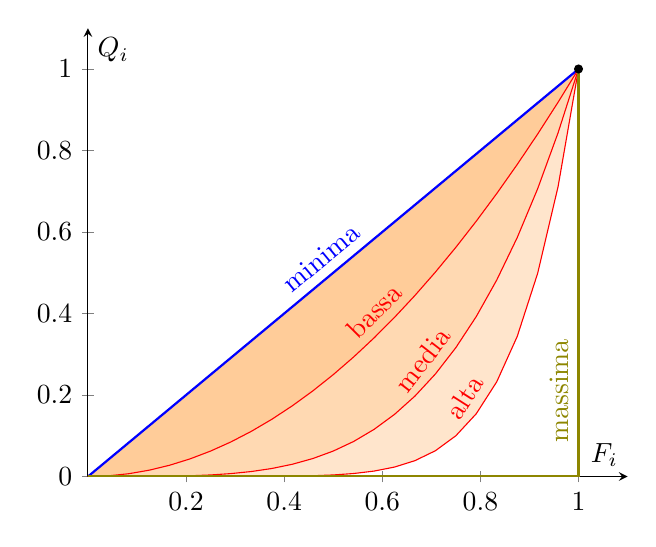
\begin{tikzpicture}
\begin{axis}[
    enlargelimits=false,
    axis lines = center,
    %axis equal,
    xlabel = $F_i$,
    ylabel = $Q_i$,
    domain = 0:1,
    xmax=1.1,
    ymin=0, ymax=1.1,
    %ytick={0,1},
    %xtick={0,1},
    extra y ticks={0},
]
\addplot[color=blue, thick, name path=A]{x} node [midway, above, sloped] (TextNode) {minima};
\addplot[color=red, name path=B]{x^2} node [midway, above, sloped] (TextNode) {bassa};
\addplot[color=red, name path=C]{x^4} node [midway, above, sloped] (TextNode) {media};
\addplot[color=red, name path=D]{x^8} node [midway, above, sloped] (TextNode) {alta};
\addplot[color=olive, thick] (0, 0) -- (1, 0);
\addplot[color=olive, thick] (1, 0) -- (1, 1) node [midway, above, sloped, xshift=-1.5cm] (TextNode) {massima};
\filldraw[color=black] (1, 1) circle (0.5mm);
\addplot [orange!20] fill between [of = A and D, soft clip={domain=0:1}];
\addplot [orange!30] fill between [of = A and C, soft clip={domain=0:1}];
\addplot [orange!40] fill between [of = A and B, soft clip={domain=0:1}];
\end{axis}
\end{tikzpicture}
\caption{Curve di Lorentz a diversi livelli di concentrazione}
\label{fig:lorentz}
\vspace*{\abovedisplayskip}
\end{figure}

\noindent Dal rapporto tra $F_i$ e $Q_i$ è possibile avere una rappresentazione grafica del livello di concentrazione del sistema. La \textit{curva} (discreta) risultante da questo rapporto è chiamata \textbf{curva di Lorentz}, rappresentata in \figurename \ \ref{fig:lorentz}.

\subsubsection{Indice di Gini (per la concentrazione)}
La curva di Lorentz è un indice qualitativo e la sua interpretazione è quindi soggettiva: quando la osserviamo ci chiediamo quanto sia ``\textit{lontana}" dalla linea indicante la concentrazione minima. Per formalizzare tale concetto possiamo considerare la somma delle differenze tra $F_i$ e $Q_i$ per $i=1$ a $i=n-1$ (per $i=n \Rightarrow F_i-Q_1=1-1=0$), normalizzando per la somma degli $F_i$. Abbiamo quindi definito l'indice di Gini per la concentrazione:
\[
\boxed{
G = \frac{\displaystyle \sum_{i=1}^{n-1}  F_i - Q_i}{\displaystyle \sum_{i=1}^{n-1} F_i}
}.
\]

\noindent L'indice di Gini è definito in $\boxed{0 \leq G \leq 1}$.

\noindent È possibile riscrivere l'indice di Gini in una forma più semplice con dei passaggi algebrici: 
\begin{gather*}
\sum_{i=1}^{n-1} F_i = \sum_{i=1}^{n-1} \frac in = \frac 1n \sum_{i=1}^{n-1} i = \frac {1}{\cancel n} \frac {(n-1) \cancel n}2 = \frac{n-1}2,
\\
\boxed{
G = \frac{2}{n-1} \sum_{i=1}^{n-1} F_i - Q_i}.
\end{gather*}

\subsection{Trasformazione dei dati}
Dato il campione $X= \{x_1, \, ..., \, x_n\}$, deriviamo l'insieme dei valori osservabili $v_1, \, ..., \, v_m$ e l'insieme delle frequenze relative associate $f'_1, \, ..., \, f'_m$. 
\textit{Trasformare i dati} significa trovare una funzione $g: X \rightarrow X'$ iniettiva che modifica ogni elemento del campione $X$ applicandolo alla funzione $g$. 
Come mai si vuole una funzione iniettiva? Poiché avendo una funzione non iniettiva si rischia di mappare due elementi diversi sullo stesso valore, ma questo non deve accadere perchè modificherebbe le frequenze relative associate ad ogni valore, e noi vogliamo una trasformazione che mantenga tutte le proprietà del campione di partenza.
Quindi per completezza ricordiamo che una funzione iniettiva è una funzione tale che presi due elementi \textbf{diversi} del dominio $v_1$ e $v_2$, essi sono associati a due elementi \textbf{diversi} del codominio, $f(v_1)$ e $f(v_2)$.

\paragraph{Traslazione}
Consideriamo la \textbf{traslazione} di un valore $k \in \mathbb{R}$: quest'ultima è una funzione $g(x) = x \pm k$ che ``sposta" in avanti o indietro tutte le misurazioni di $k$. Questa trasformazioni viene utilizzata generalmente nel caso in cui i dati siano di dimensioni molto grandi o molto piccole, in modo da trasformarli in dati che possono essere trattati più facilmente.

\paragraph{Scalatura}
Consideriamo ora la \textbf{scalatura} di un fattore $h \in \mathbb{R^+}$: quest'ultima è una funzione $g(x) = hx$. \\
A differenza della traslazione, tutti gli indici analizzati fin'ora sono sensibili alla scalatura.
\[
\begin{cases}
h > 1:  \textit{i dati vengono dilatati} \\
0 < h < 1:  \textit{i dati vengono compressi} \\
h < 0:  \textit{i dati oltre a subire una dilatazione o compressione vengono specchiati} \\
\end{cases} \! \! \! \! \! \! .
\]

Sfruttando la scalatura è possibile fare in modo che il valore \textbf{minimo} sia $0$ e che non vi sia una limitazione sul valore massimo, e questo è possibile scalando per il valore minimo delle osservazioni.

\begin{table}[h]
\centering
\vspace{\abovedisplayskip}
\begin{tabular}{r l|cc}
    \multicolumn{2}{c}{\textbf{Indice}} \vline & $g(x) = x \pm k$ & $g(x) = hx$ \\
    \hline
    Media & $\overline x$ & $\overline x \pm k$ & $h \overline x$ \\
    Mediana & $m_x$ & $m_x \pm k$ & $h m_x$ \\
    Moda & $M_x$ & $M_x \pm k$ & $h M_x$ \\
    Quantile & $q_x$ & $q_x \pm k$ & $h q_x$ \\
    \hline
    Varianza & $\mathnormal{s}_x^2$ & $\mathnormal{s}_x^2$ & $h^2 \mathnormal{s}^2_x$ \\
    Dev. std. & $\mathnormal{s}_x$ & $\mathnormal{s}_x$ & $|h|\mathnormal{s}_x$ \\
    Range & $r_x$ & $r_x$ & $hr_x$ \\
    IQR & $\text{IQR}_x$ & $\text{IQR}_x$ & $h \text{IQR}_x$
\end{tabular}
\vspace{\abovedisplayskip}
\end{table}

\paragraph{Cambiamento di origine e scala}
Applicare delle trasformazioni ai dati significa cambiare sistema di riferimento, mappando un range $(a, \, b)$ in un range $(c, \, d)$. 

\begin{figure}[h]
\vspace*{\abovedisplayskip}
\centering
\begin{tikzpicture}
\begin{axis}[
    enlargelimits=false,
    axis lines = center,
    %axis equal,
    xlabel = $x$,
    ylabel = $x'$,
    domain = -1:1.75,
    xmin=-0.25, xmax=1.50,
    ymin=-0.25, ymax=1.50,
    xtick={0.25, 1.25},
    xticklabels={$a$, $b$},
    ytick={0.25, 1.25},
    yticklabels={$c$, $d$}
]
\addplot[color=blue, ultra thick, domain=0.25:1.25]{x};
\addplot[color=blue]{x};
\filldraw[color=blue] (0.25, 0.25) circle (0.5mm);
\filldraw[color=blue] (1.25, 1.25) circle (0.5mm);

\end{axis}
\end{tikzpicture}
\caption{Modifica del sistema di riferimento con trasformazione lineare}
\label{fig:transform}
\vspace*{\abovedisplayskip}
\end{figure}

\noindent Osservando il grafico a \figurename \ \ref{fig:transform}, la funzione che mappa $(a,b)$ in $(c,d)$ è una retta, la cui equazione la si ricava con la formula della retta passante tra due punti: \begin{align*}
f(x) = x^i = 
\frac{x'-c}{d-c} = \frac{x-a}{b-a} \Rightarrow
x' = c + \frac{d-c}{b-a}(x-a)
\end{align*}

\noindent La \textbf{standardizzazione} (o \textbf{normalizzazione}) è un caso particolare di cambiamento di origine e scala, e consiste nell’applicare una scala il cui fattore è uguale alla deviazione standard dei valori, per poi traslare verso sinistra rispetto alla media dei valori. Definiamo per standardizzazione una operazione di trasformazione lineare di variabile che prevede una centratura (sottrarre la media) e una uniformazione (dividere per la deviazione standard). Tramite la centratura otteniamo una nuova variabile con media (o valore atteso) zero e tramite l'uniformazione togliamo l'unità di misura ed esprimiamo la variabile utilizzando come unità di misura la deviazione standard. Per esempio il valore standardizzato di $\overline{x} + 2,5 \cdot s_x = 2,5$. In questo modo i valori positivi sono valori sopra media e quelli negativi sono valori sotto media \[
(a, \, b) \rightarrow (-1, \, +1) \Rightarrow x' = 2 \frac{x-a}{b-a} -1 \Leftrightarrow x' = \frac{x - \overline x}{\mathnormal{s}_x}
\]

\noindent La trasformazione di standardizzazione trasforma pertanto l’insieme dei valori in un altro insieme
di valori la cui media è $0$ e la cui varianza è $1$.
Nel caso in cui il campione segua la \textbf{distribuzione approssimativamente normale} e venga applicata questa trasformazione si avrà che:
\begin{itemize}
    \item approssimativamente il 68\% delle osservazioni dista dalla media campionaria sta tra -1 e 1;
    \item approssimativamente il 95\% delle osservazioni dista dalla media campionaria sta tra -2 e 2;
    \item approssimativamente il 99.7\% delle osservazioni dista dalla media campionaria sta tra -3 e 3.
\end{itemize}

\begin{dimostrazione}[Media campionaria pari a $0$]
Supponiamo di avere un campione di dati $(x_1, x_2, \ldots, x_n)$ con media campionaria $(\overline{x})$ e deviazione standard campionaria $(s_x)$.
\begin{align*}
\text{Media campionaria di }\frac{x - \overline{x}}{s_x} & = \frac{1}{n} \sum_{i=1}^{n} \left(\frac{x_i - \overline{x}}{s_x}\right) \\
& = \frac{1}{n} \sum_{i=1}^{n} \left(\frac{x_i}{s_x} - \frac{\overline{x}}{s_x}\right) \\
& = \frac{1}{n} \left(\frac{1}{s_x} \sum_{i=1}^{n} x_i - \frac{1}{s_x} \sum_{i=1}^{n} \overline{x}\right) \\
& = \frac{1}{n} \left(\frac{1}{s_x} \sum_{i=1}^{n} x_i - \frac{n\overline{x}}{s_x} \right) \\
& = \frac{1}{n} \left(\frac{n\overline{x}}{s_x} - \frac{n\overline{x}}{s_x}\right) \\
& = \frac{1}{n} \left(0\right) \\
& = 0
\end{align*}
\end{dimostrazione}

\begin{dimostrazione}[Varianza campionaria pari a $1$]
\begin{align*}
\text{Varianza campionaria di }\frac{x - \overline{x}}{s_x} & = \frac{1}{n-1} \sum_{i=1}^{n} \left(\frac{x_i - \overline{x}}{s_x}\right)^2 \\
& = \frac{1}{s_x^2} \frac{1}{n-1} \sum_{i=1}^{n} \left(x_i - \overline{x}\right)^2  \\
& = \frac{1}{s_x^2} \underbrace{\frac{1}{n-1} \sum_{i=1}^{n} \left(x_i - \overline{x}\right)^2}_{s_x^2} \\
& = \frac{1}{\cancel{s_x^2}} \cdot \cancel{s_x^2} \\
& = 1
\end{align*}
\end{dimostrazione}

\paragraph{Trasformazioni logaritmiche}
A volte i valori di una variabile osservata sono molto grandi oppure molto distanziati. In questi casi può essere utile considerare non tanto il valore originale ma, pensando a tale valore come potenza di una data base, ragionare in termini del relativo esponente. Ciò corrisponde ad applicare una trasformazione logaritmica del seguente tipo:
\[
x \Rightarrow x' = \log x
\]
Nel caso i valori siano molto distanziati tra loro e caratterizzati da una distribuzione di frequenza unimodale fortemente asimmetrica, la trasformazione logaritmica permette di ottenere una distribuzione di frequenza più simmetrica.

\subsection{Analisi della varianza}
Dato un campione $X$ può essere interessante suddividerlo in gruppi e osservare le differenze tra un gruppo e l'altro.
\noindent Ad esempio, dato un campione che contiene i redditi di una certa professione si potrebbe dividere e confrontare per regione, per genere o per fascia d'età.
\newline Indichiamo con $x_i^g$ l'$i$-esimo campione e $n_g$ il numero di osservazioni del $g$-esimo dei $1, \, \dots, \, G$ gruppi.
L'indice $i$ varia quindi tra $1$ e $n_g$:
$x_1^1, \, x_2^1, \, \dots, \, x_{n_1}^1, \, \dots, \, x_{1}^{G}, \, \dots, \, x_{n_G}^G$.
Se si è interessati a valutare l’ipotesi che i valori delle medie nei vari gruppi non siano sensibilmente differenti, per esempio perché si vuole dimostrare che il reddito non sia troppo diverso in un gruppo di città, oppure per dimostrare l’efficacia di un dato trattamento medico, è possibile applicare un metodo chiamato \textbf{ANOVA} (\textbf{ANalysis Of VAriance}). L’idea alla base di questo metodo è che se non vi sono sostanziali differenze tra i gruppi considerati, allora calcolare la varianza all’interno di un gruppo qualsiasi non dovrebbe portare a un risultato molto dissimile da quello ottenuto effettuando il calcolo su tutti i dati a disposizione.
Si definisce la media campionaria di un gruppo \[
\overline{x}^g = \frac{1}{n_g} \sum_{i=1}^{n_g}{x_i^g};
\] 
di conseguenza, è possibile ridefinire la media campionaria come \[
\overline{x} = \frac{1}{n} \sum_{g=1}^G{\sum_{i=1}^{n_g}{x_i^g}} = \frac{1}{n} \sum_{g=1}^G{n_g \overline{x}^g}.
\]
Si possono definire ora tre indici di variazione, in stretta correlazione tra loro:
\begin{itemize}
    \item (\textit{total}) $\operatorname{var}_T = \dfrac{\text{SS}_\text{T}}{n-1}$, con $\displaystyle \text{SS}_\text{T} = \sum_{g=1}^G \sum_{i=1}^{n_g} (x_i^g - \overline{x})^2$: la varianza totale del campione;
    \item (\textit{within}) $\operatorname{var}_W = \dfrac{\text{SS}_\text{W}}{n-G}$, con $\displaystyle \text{SS}_\text{W} = \sum_{g=1}^G \sum_{i=1}^{n_g} (x_i^g - \overline{x}^g)^2$: la varianza di ogni elemento del gruppo;
    \item (\textit{between}) $\operatorname{var}_B = \dfrac{\text{SS}_\text{B}}{G-1}$, con $\text{SS}_\text{B} = \displaystyle \sum_{g=1}^G n_g(\overline{x}^g - \overline{x})^2$; la varianza tra ogni gruppo e l'insieme completo.
\end{itemize}
Vale sempre la seguente regola:
\[
\boxed{\text{SS}_\text{T} = \text{SS}_\text{W} + \text{SS}_\text{B}}.
\]
\mdfsetup{skipabove=0pt,skipbelow=0pt}

\begin{dimostrazione}[$\text{SS}_\text{T} = \text{SS}_\text{W} + \text{SS}_\text{B}$]
\begin{align*}
\textnormal{SS}_\textnormal{T} &= {\sum}_g {\sum}_i (x_i^g - \overline{x})^2 = \\
&= {\sum}_g \sumi ((x_i^g)^2 - 2x_i^g\overline{x} + (\overline{x})^2)= \\
\intertext{\indent completo il quadrato di $(x_i^g - \overline{x}^g)^2$ per ottenere $\textnormal{SS}_\textnormal{W}$ e riscrivo le sommatorie}
&= {\sum}_g 
\sumi \left(\cancel{(x_i^g)^2} - 2x_i^g\overline{x} + (\overline{x})^2
\green{\cancel{+(\overline x^g)^2}} \red{-(\overline x^g)^2} \green{+2x_i^g\overline{x}^g} \red{\cancel{-2x_i^g\overline{x}^g}} 
\right )= \\
&= \underbrace{{\sum}_g \sumi \left(x_i^g - \overline x^g \right)^2}_{=\textnormal{SS}_\textnormal{W}} + 
{\sum}_g \sumi \left ( (\overline x)^2 - (\overline x^g)^2 - 2  x^g_i \overline x + 2 x^g_i \overline x^g \right ) = \\
&= \textnormal{SS}_\textnormal{W} + {\sum}_g \left (
n_g(\overline x)^2 - n_g (\overline x^g)^2 - 2 \overline x \sumi x^g_i + 2\overline x^g \sumi x^g_i
\right ) = \\
\intertext{\indent essendo $\sumi x_i^g = n_g \overline x$, raccolgo $n_g$}
&= \textnormal{SS}_\textnormal{W} + {\sum}_g n_g \left ( 
(\overline x) ^ 2 - (\overline x^g) ^2 - 2 \overline x \overline x^g + 2 (\overline x^g)^2  
\right ) = \\
\intertext{\indent ho quindi ottenuto il quadrato della formula di $\textnormal{SS}_\textnormal{B}$}
&= \textnormal{SS}_\textnormal{W} + \underbrace{{\sum}_g n_g \left ( 
\overline x^g - \overline x
\right )^2}_{\textnormal{SS}_\textnormal{B}} = \\
&= \textnormal{SS}_\textnormal{W} + \textnormal{SS}_\textnormal{B} = \textnormal{SS}_\textnormal{T} \tag*{$\blacksquare$}
\end{align*}

%\endgroup
\end{dimostrazione}

\subsection{Alberi di decisione}
Gli indici di eterogeneità sono alla base della costruzione di un interessante classificatore chiamato \textbf{albero di decisione}. Un albero di decisione assegna \textit{oggetti} a \textit{classi}, dove un oggetto è descritto tramite un'osservazione che consiste in un vettore di valori per degli attributi prefissati. 
\newline \newline
Il procedimento di classificazione procede nel modo seguente: si considera la radice dell'albero che è contrassegnata da una condizione che coinvolge i valori di uno o più attributi per l'oggetto che si vuole classificare; a seconda del valore di questa condizione, si percorre una delle due frecce partenti dalla radice. Se il nodo a cui si arriva è un nodo terminale, in tale nodo è indicata la classe assegnata all'oggetto, altrimenti il nodo riporta un'altra condizione da valutare, iterando il comportamento precedente fino a che non si raggiunge una foglia, in questo modo si determina una classe per l'oggetto. 
\newline \newline
Quindi un albero di decisione è un albero in cui tutti i nodi interni vengono etichettati con dei criteri booleani che si possono testare sui dati mentre le foglie vengono etichettate con un esito del processo di classificazione.

\subsubsection{Alberi binari}
L'albero viene costruito sulla base di una domanda che lo spezza in due, quindi il primo passo per la costruzione è guardare il dataset, visualizzare gli attributi che abbiamo a disposizione e formulare la domanda sull'attributo che permette di spezzare il dataset in due parti più o meno uguali. Per controllare quanto la domanda posta sia stata buona, è necessario trovare un indice di eterogeneità per poi calcolare la media pesata sui due gruppi.
\newline
Per proseguire con la creazione dell'albero di decisione, bisognerebbe applicare nuovamente il processo di ottimizzazione al gruppo che non ha ottenuto la massima omogeneità, e ripetere il processo finché non la si ottiene in tutti i gruppi.
\newline
Una volta finita la creazione del nostro albero possiamo passargli un oggetto e in base alle condizioni create, gli verrà assegnata una classe. Ovviamente, seppur è possibile lavorare con dati categorici per la costruzione di alberi di decisione, è necessario che questi vengano convertiti in valori numerici in quanto altrimenti la libreria per generare l'albero non funzionerebbe.

\subsection{Analisi di classificatori}
Immaginiamo di avere a disposizione un classificatore \textit{binario}, costruito cioè per discriminare tra due classi che indicheremo come positiva e negativa. Possiamo valutare la bontà di questo classificatore calcolando il numero di casi che vengono classificati in modo errato; notiamo però che ci sono due possibili modi di sbagliare la classificazione:
\begin{itemize}
    \item un esempio positivo viene classificato come negativo, dando luogo a un cosiddetto falso negativo;
    \item un esempio negativo viene classificato come positivo, e in questo caso si parla di falso positivo.
\end{itemize}
In alcuni casi il peso dato a un errore che coinvolge un falso positivo equivale a quello dato a un falso negativo, ma non è sempre così. Se per esempio il procedimento di classificazione mira a determinare i portatori di una grave malattia contagiosa, un falso positivo sta a indicare un individuo sano che viene erroneamente classificato come malato; un falso negativo corrisponde invece a un individuo contagioso classificato come sano e quindi a una falla nel contenimento di una potenziale epidemia.
\newline \newline
La \textbf{matrice di confusione} è una matrice in cui una dimensione è legata alle predizione effettuate mentre sulle colonne il valore effettivo. Abbiamo quindi per ogni cella una possibile predizione che può essere:

\begin{center}
\begin{tabular}{ | m{3cm} | c | c | c | c | } 
    \hline
    \multicolumn{2}{|c|}{} & \multicolumn{2}{|c|}{Effettivo} \\
    \cline{3-4}
    \multicolumn{2}{|c|} {}
    & Positivi & Negativi\\
    \hline
    \multirow{2}{*}{Predizione}
    & Positivo & True Positive (VP) & False Positive (FP) \\
    \cline{2-4}
    & Negativo & False Negative (FN) & True Negative (VN) \\
    \hline
    \rowcolor{green!50}
    \multicolumn{2}{| c |}{Totals}
    & TP & TN \\
    \hline
\end{tabular}
\end{center}

La \textbf{sensibilità} è la capacità del classificatore di predire bene i positivi $\dfrac{\text{VP}}{\text{TP}}$ mentre la \textbf{specificità} è la capacità del classificatore di predire bene i negativi $\dfrac{\text{VN}}{\text{TN}}$
\newline
Una volta calcolati i valori, è possibile valutare il classificatore in funzione della posizione assunta dal punto di coordinate $(1 - \text{specificità}, \text{sensibilità})$

\subsubsection{Classificatori costanti} 
Sono i classificatori che associano indiscriminatamente gli oggetti nella classe positiva; quello che succede è che tutti i positivi sono predetti correttamente mentre tutti i negativi sono predetti falsamente. La sensibilità in questo caso sarà $1$ e la specificità sarà $0$. Lo stesso vale per i classificatori che associano indiscriminatamente gli oggetti nella classe negativa. (\figurename \ \ref{fig:classificatori}a)

\subsubsection{Classificatori ideali}
Sono i classificatori che hanno come coordinate $(0, 1)$ e significa che il $100\%$ dei valori positivi viene correttamente classificato e lo stesso per i negativi; quindi è il classificatore che non commette errore. (\figurename \ \ref{fig:classificatori}b)

\subsubsection{Classificatori casuali}
Sono i classificatori che corrispondono al punto $\left(\dfrac{1}{2},\dfrac{1}{2}\right)$, quindi assegna un generico oggetto a una classe scelta uniformemente a caso, per esempio lanciando una moneta. (\figurename \ \ref{fig:classificatori}c)

\subsubsection{Classificatori a soglia}
Sono i classificatori effettuano il procedimento di classificazione di un generico oggetto calcolando una quantità e verificando che quest'ultima sia superiore a una soglia prefissata. La quantità varierà in funzione dell'oggetto considerato mentre la soglia resterà uguale. Gli indici di sensibilità e specificità possono essere utilizzati proprio per fissare il valore della soglia: indicando con $\theta$ un generico valore per la soglia e identificato un intervallo $[\theta_{\text{min}}, \theta_{\text{max}}]$, si può considerare un'opportuna discretizzazione finita di tale intervallo $D = \{\theta_0 = \theta_{\text{min}}, ..., \theta_n = \theta_{\text{max}}\}$. Per ogni $\theta \in D$ è poi possibile calcolare la sensibilità e la specificità del classificatore e disegnare sul piano cartesiano il punto corrispondente; il risultato è una traiettoria che prende il nome di \textbf{curva ROC}. (\figurename \ \ref{fig:classificatori}d) L'andamento di una curva ROC ha sempre l'origine e il punto $(1, 1)$ come estremi. Infatti quando la soglia assume rispettivamente i suoi valori minimo e massimo il classificatore ha un output costante. Il grafico della curva viene inoltre utilizzato per valutare la bontà del classificatore indipendentemente da uno specifico valore della soglia; il valore di tale area viene indicato con la sigla \textbf{AUC} ("Area Under the ROC Curve"): più si avvicina a $1$ , più il classificatore ha un comportamento che approssima quello del caso ideale CI.

\begin{figure}[h]
    \centering
\subfloat[Classificatore constanti]{ 
    \resizebox{4cm}{!}{
        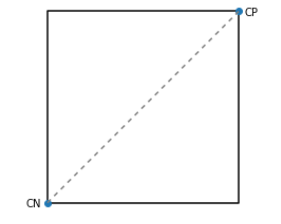
\includegraphics{images/c_costanti.png}
    }
}
\subfloat[Classificatore ideale]{
    \resizebox{4cm}{!}{
        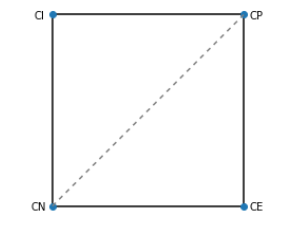
\includegraphics{images/c_ideali.png}
    }
}
\subfloat[Classificatore casuali]{
    \resizebox{4cm}{!}{
        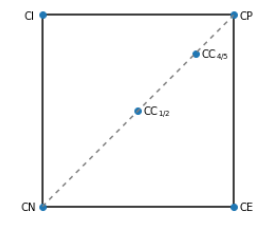
\includegraphics{images/c_casuali.png}
    }
}
\subfloat[Classificatore soglia]{
    \resizebox{4cm}{!}{
        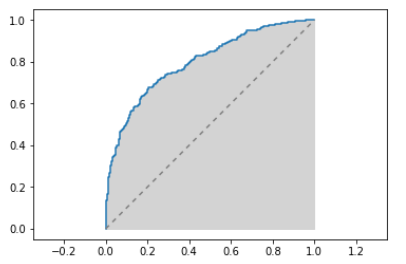
\includegraphics{images/c_soglia.png}
    }
}
    \caption{Rappresentazione grafica dei classificatori}
    \label{fig:classificatori}
    \vspace{\abovedisplayskip}
\end{figure}

\subsection{Altri grafici}
Vediamo ora per ogni grafico, per quali tipi di dati è sensato utilizzarlo e perché.

\subsubsection{Grafico a barre}
I grafici a bastoncini/barre servono a descrivere insiemi di dati che hanno un numero relativamente basso di valori distinti; se questo numero diventa troppo grande, rendono inefficaci questi tipi di grafici e quindi è utile suddividere i dati in classi disgiunte e considerare quanti valori cadono in ogni classe. Questo tipo di grafico è possibile utilizzarlo sia per dati quantitativi discreti, sia per i dati qualitativi.

\subsubsection{Istogramma}
L'istogramma è un grafico a barre che rappresenta le frequenze nelle varie classi. Quando gli insiemi di dati hanno troppi valori distinti, vengono suddivisi i valori in gruppi o classi, per poi rappresentare con un grafico il numero di valori dei dati che cadono in ciascuna classe. La rappresentazione standard della libreria di matplotlib per l'istogramma pone sull'asse delle ordinate la frequenza assoluta e non quella relativa. Il numero di classi dovrebbe essere un compromesso tra:
\begin{itemize}
    \item scegliere poche classi al costo di perdere molte informazioni sui valori effettivi in una classe
    \item scegliere troppe classi, ottenendo frequenze troppo basse all'interno di ogni classe
\end{itemize}

\noindent Questo tipo di grafico è possibile utilizzarlo sia per i dati quantitativi, che per i dati qualitativi. È uno strumento importante perché ci permette di capire:
\begin{itemize}
    \item il grado di simmetria dei dati
    \item il grado di dispersione dei dati
    \item l'eventuale presenza di intervalli con un'alta concentrazione
    \item l'eventuale presenza di vuoti nei dati
\end{itemize}

\noindent Un diverso tipo di rappresentazione di un insieme di dati è il grafico delle \textbf{frequenze cumulative} (\textbf{ECDF}). Un insieme di dati si dice \textbf{normale} se ha il \textbf{punto di massimo} ed è \textbf{simmetrico} in corrispondenza dell'intervallo centrale e se l'istogramma risulti a forma di campana.

\subsubsection{Simmetria}
Quando le frequenze, visualizzate a seconda dei casi tramite un grafico a barre o un istogramma, tendono a distribuirsi in modo simmetrico rispetto al valore della media campionaria si dice che il campione segue una distribuzione \textit{approssimativamente simmetrica} (\figurename \ \ref{fig:simmetire}a). Tra le distribuzioni approssimativamente simmetriche, un ruolo particolare spetta alle cosiddette distribuzioni approssimativamente normali, in cui la simmetria è accompagnata da una forma a campana del grafico delle frequenze. In questo tipo di distribuzioni i dati si concentrano attorno alla media campionaria secondo la seguente \textbf{regola empirica}:
\begin{itemize}
    \item approssimativamente il $68\%$ delle osservazioni dista dalla media campionaria non più di una deviazione standard campionaria;
    \item approssimativamente il $95\%$ delle osservazioni dista dalla media campionaria non più di due deviazioni standard campionarie;
    \item approssimativamente il $99.7\%$ delle osservazioni dista dalla media campionaria non più di tre deviazioni standard campionarie.
\end{itemize}
L’\textbf{asimmetria} in una distribuzione si può invece presentare in due diverse modalità:
\begin{itemize}
    \item tende a essere presente una \textit{coda} nella parte destra della distribuzione delle frequenze,
    evidenziata da valori più bassi e da un baffo destro sensibilmente più lungo nel box plot; in questo caso si parla quindi di distribuzione asimmetrica a destra (skew a destra) (\figurename \ \ref{fig:simmetire}b)
    \item viceversa, è possibile che la \textit{coda} della distribuzione sia a sinistra, quindi si parla di asimmetria a sinistra (\figurename \ \ref{fig:simmetire}c)
\end{itemize}

\begin{figure}[h]
    \centering
\subfloat[Simmetria]{ 
    \resizebox{5cm}{!}{
        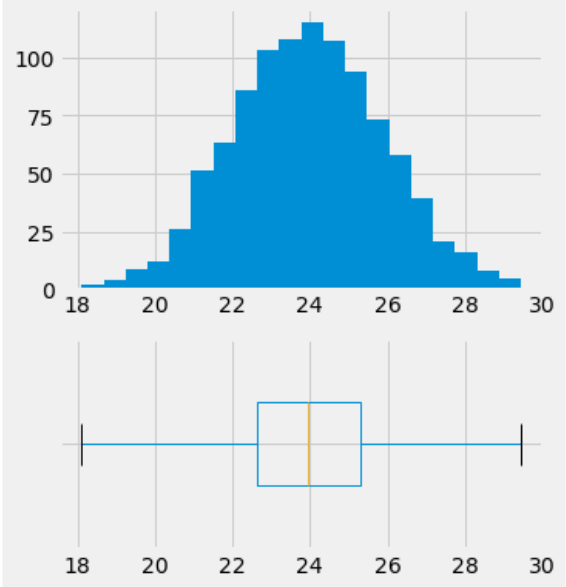
\includegraphics{images/simmetria.png}
    }
}
\subfloat[Asimmetria a destra]{
    \resizebox{5cm}{!}{
        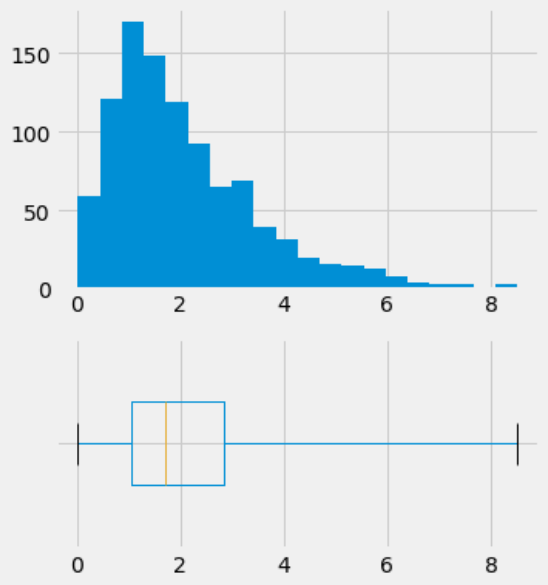
\includegraphics{images/asimmetria_destra.png}
    }
}
\subfloat[Asimmetria a sinistra]{
    \resizebox{5cm}{!}{
        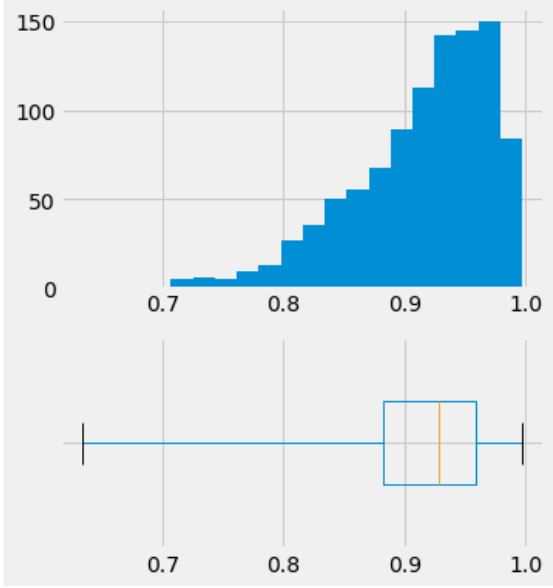
\includegraphics{images/asimmetria_sinistra.png}
    }
}
    \caption{Rappresentazione grafica delle simmetrie tramite istogramma e box plot}
    \label{fig:simmetire}
    \vspace{\abovedisplayskip}
\end{figure}

\hspace{1cm}

\paragraph{Forte simmetria}
Nel caso in cui vi sia una forte simmetria tra i dati, il box plot generato a partire da essi si presenterà come in figura \ref{fig:forte_simmetria}. Lo spazio tra un quartile e l'altro è uguale (o quasi), e ciò indica che vi è una certa uniformità tra i dati.
\newline
Si noti come è possibile passare da un box plot a diversi grafici abbastanza diversi tra loro, ma tutti corretti; ciò può avvenire anche per i casi precedenti.
Nella figura \ref{fig:forte_simmetria} la mediana si trova sull'asse delle ascisse nella parte centrale, nel punto in cui sia a destra che a sinistra di essa vi sia la stessa quantità di dati.
\newline

\begin{figure}[h]
    \centering
    \resizebox{15cm}{!}{
        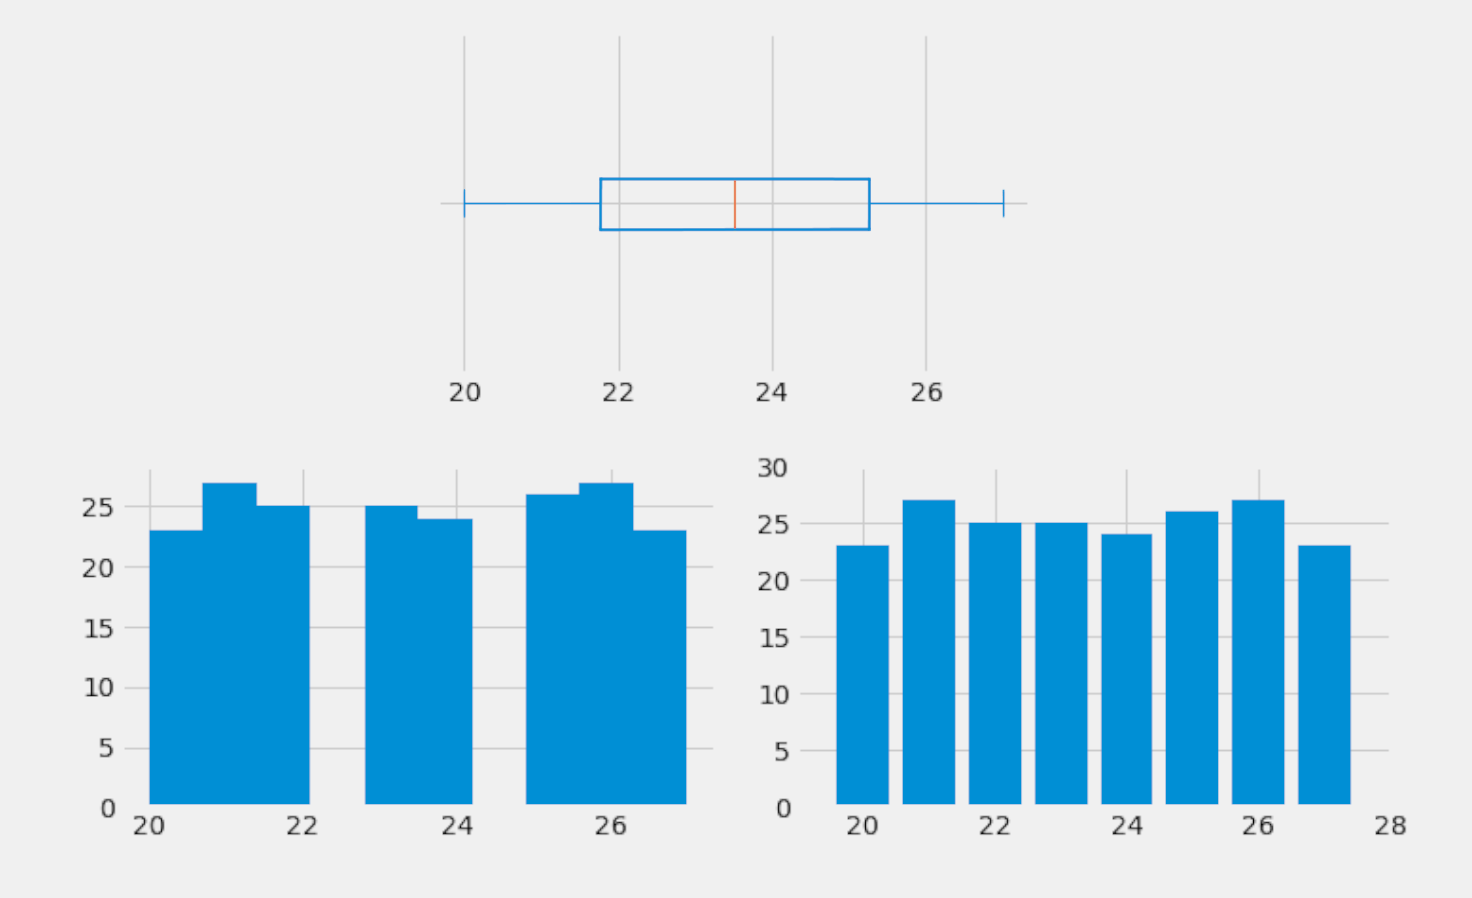
\includegraphics{images/perf_simmetria.png}
    }
    \caption{Rappresentazione grafica nel caso di forte simmetria}
    \label{fig:forte_simmetria}
    \vspace{\abovedisplayskip}
\end{figure}

\subsubsection{QQ-plot}
Un diagramma quantile-quantile è una rappresentazione grafica che considera due campioni al fine di valutare la validità dell’ipotesi che i campioni stessi seguano una medesima distribuzione. Questi diagrammi si basano sul fatto che i quantili campionari rappresentano l’approssimazione di quantili teorici i quali individuano univocamente la distribuzione dei dati. Pertanto, se due campioni hanno un’uguale distribuzione, allora estraendo da entrambi il quantile di un livello fissato si dovranno ottenere due numeri molto vicini in quanto essi rappresentano approssimazioni diverse di uno stesso valore. Il fatto che in ogni coppia considerata i due quantili sono molto simili tra loro fa sì che i punti ottenuti si allineino approssimativamente sulla bisettrice del primo e del terzo quadrante.
\newline \newline
Una standardizzazione dei dati permette di confinare il grafico ottenuto in prossimità dell'origine in modo tale da rendere più semplice accorgersi di eventuali valori fuori scala

% Calcolo delle probabilità
\newpage
\section{Calcolo delle probabilità}
Il calcolo delle probabilità è una branca della matematica che permette la creazione di modelli di situazioni di incertezza.

\subsection{Calcolo combinatorio}
Il calcolo combinatorio studia come e in quanti modi è possibile aggregare degli elementi diversi secondo dei criteri di aggregazione, quindi determina come e in quanti modi è possibile strutturare l'insieme.

\subsubsection{Principio fondamentale del calcolo combinatorio o  principio di enumerazione}
Dati due esperimenti con rispettivamente $n$ e $m$ esiti possibili (da $1$ a $n$ e $m$) e la tupla $(i, \, j)$ indicante l'esito combinato di un esito $i$ del primo e $j$ del secondo esperimento, allora il \textbf{numero totale di esiti} combinati possibili è $n \cdot m$. Il principio fondamentale del calcolo combinatorio si può generalizzare per un numero arbitrario di esperimenti.

\subsubsection{Disposizioni}
Si vogliono \textbf{ordinare} $n$ elementi di un insieme $A$ in $k$ posizioni, con $k \leq n$.
In questo caso \textbf{l'ordine conta!}

\paragraph{Disposizioni semplici}
Se l'insieme \textbf{non contiene elementi ripetuti} allora il numero di disposizioni semplici è \[
\boxed{
d_{n, \, k} = n(n-1)(n-2) \cdots (n-k+1) \frac{(n-k)!}{(n-k)!} = \frac{n!}{(n-k)!}
}.
\]
Le disposizioni sono una generalizzazione delle permutazioni: infatti, in queste ultime, $n$ e $k$ coincidono.

\paragraph{Disposizioni con ripetizione}
Analogamente, se l'insieme \textbf{contiene elementi ripetuti} allora il numero di disposizioni con ripetizione è: \[
\boxed{
D_{n, \, k} = n^k
}.
\]
infatti in questo caso per ogni posizione posso scegliere tra $n$ elementi.

\subsubsection{Permutazioni}
Dato un insieme $A = \{ a_1, \, \dots, \, a_n \}$ di $n$ elementi, si vuole trovare il numero di sequenze di quest'ultimi, costruite usando gli elementi di $A$, che possono essere o meno ripetuti. \\

\noindent Visualmente, assumiamo di voler contare tutti i modi con i quali possiamo riempire uno scaffale di $n$ posti con $n$ elementi.

\begin{figure}[h]
\vspace{\abovedisplayskip}
\centering
\begin{tikzpicture}
% scaffale
\draw[gray] (0, 0) -- (6, 0);
\foreach \i in {0, ..., 2} {
    \draw[gray] (\i, 0) -- (\i, 0.75);
}
\node[] at (3.5, 0.37) {$\dots$};
\draw[gray] (5, 0) -- (5, 0.75);
\draw[gray] (6, 0) -- (6, 0.75);

% posti
\node[] at (0.5, -0.37) {1°};
\node[] at (1.5, -0.37) {2°};
\node[] at (3.5, -0.37) {$\dots$};
\node[] at (5.5, -0.37) {$n$};
\end{tikzpicture}
\end{figure}

Se ci si pensa questo non è altro che il caso in cui si ha una disposizione avente $n = k$

\paragraph{Permutazioni semplici}
Se la permutazione \textbf{non contiene ripetizioni}, ovvero contiene ogni elemento di $A$ una e una sola volta, si parla di \textbf{permutazioni semplici}. Ad esempio, dato l'insieme $A = \{a, \, b\}$, le possibili permutazioni sono $2$: $\{a, \, b\}$ e $\{b, \, a\}$. Notare come le permutazioni abbiano gli stessi elementi ma sono comunque considerate diverse: questo avviene perché nelle permutazioni l'ordine è rilevante. \\
Indicando con $p_n$ il numero di permutazioni semplici di un insieme di $n$ elementi, allora \[ 
\boxed{p_n = \prod_{i=1}^n i = n!}.
\]
\paragraph{Permutazioni con ripetizione}
Se l'insieme contiene degli elementi ripetuti, una volta raggruppati gli elementi unici in $k$ gruppi il numero di \textbf{permutazioni con ripetizione} è \[
\boxed{
    P_{n_1, \, \dots \, , n_k} =
    \frac{n!}{n_1! \cdots n_k!}
}.
\]
Le permutazioni con ripetizione sono anche chiamate \textbf{permutazioni di oggetti distinguibili a gruppi}.

\subsubsection{Combinazioni}
Utilizzando la notazione di Python, possiamo vedere il risultato delle disposizioni come delle \textit{liste} (poiché l'ordine conta) mentre le combinazioni come degli \textit{insiemi}, perché \textbf{l'ordine non conta}.
Anche in questo caso si vogliono ordinare $n$ elementi in $k$ posti, senza però che l'ordine conti.

\paragraph{Combinazioni semplici}
Il numero di combinazioni semplici \textbf{senza ripetizione} è \[
\boxed{
c_{n, \, k} = \frac{d_{n, \, k}}{p_k} = \frac{\frac{n!}{(n - k)!}}{k!} = \frac{n!}{(n-k)!} \frac{1}{k!} = \frac{n!}{(n-k)!k!} = \binom{n}{k}
}.
\]
Notare come, per definizione, $c_{n, k} < d_{n, \, k}$, inoltre è importante sottolineare che $k!$ non è mai uguale a $0$, infatti non avrebbe senso perché come sarebbe possibile ordinare $n$ elementi in $0$ posti? non si può.
\\
Ma nel caso in cui $k!$ fosse negativo? anche in questo caso non è possibile per lo stesso discorso, infatti come sarebbe possibile ordinare $n$ elementi in $k$ posti, se ad un certo punto gli elementi da disporre terminano.
\\
Sfruttiamo un esempio per capire cosa succede:
Se abbiamo $5$ persone da disporre in una sala da $100$ posti come possiamo fare?
Concettualmente il concetto di "elementi da disporre" e "posti" si invertono, infatti è come se dovessimo trovare in quanti modi è possibile assegnare $5$ posti a sedere a un gruppo di $100$ persone, ecco qui che $k$ non può essere minore di $n$.
\\
\\
Il \textbf{coefficiente binomiale} è utile per dimostrare un'importante proprietà degli insiemi:
\begin{teorema}
Sia $\mathcal A$ un insieme e $\mathcal{P}(\mathcal A)$ il suo insieme delle parti, allora $|\mathcal{P}(\mathcal A)| = 2^{|\mathcal A|}$.
\end{teorema}
\begin{dimostrazione}
Sia $|\mathcal A| = n$, allora \[|\mathcal{P}(\mathcal A)| = \sum\limits_{k=0}^{n}{\textnormal{(\# insiemi formati da $k$ elementi)}} = \sum\limits_{k=1}^n{\binom{n}{k}} + 1 = \sum\limits_{k=0}^n{\binom{n}{k}} 1^k 1^{n-k},
\]
ma questa è la formula del binomio di Newton: \[
(a+b)^n = \sum\limits_{k=0}^n{\binom{n}{k}} a^k b^{n-k},\] dove $a=b=1$;
otteniamo quindi: \begin{align*}
|\mathcal{P}(\mathcal A)| = (1+1)^n = 2^n = 2^{|\mathcal A|}. \tag*{$\blacksquare$} \end{align*}
\end{dimostrazione}

\paragraph{Combinazioni con ripetizione}
Il numero di combinazioni \textbf{con ripetizione} è \[
\boxed{
C_{n, \, k} = \binom{n+k-1}{k}
}.
\]

\subsubsection{Riassunto}
\begin{figure}[h]
\centering
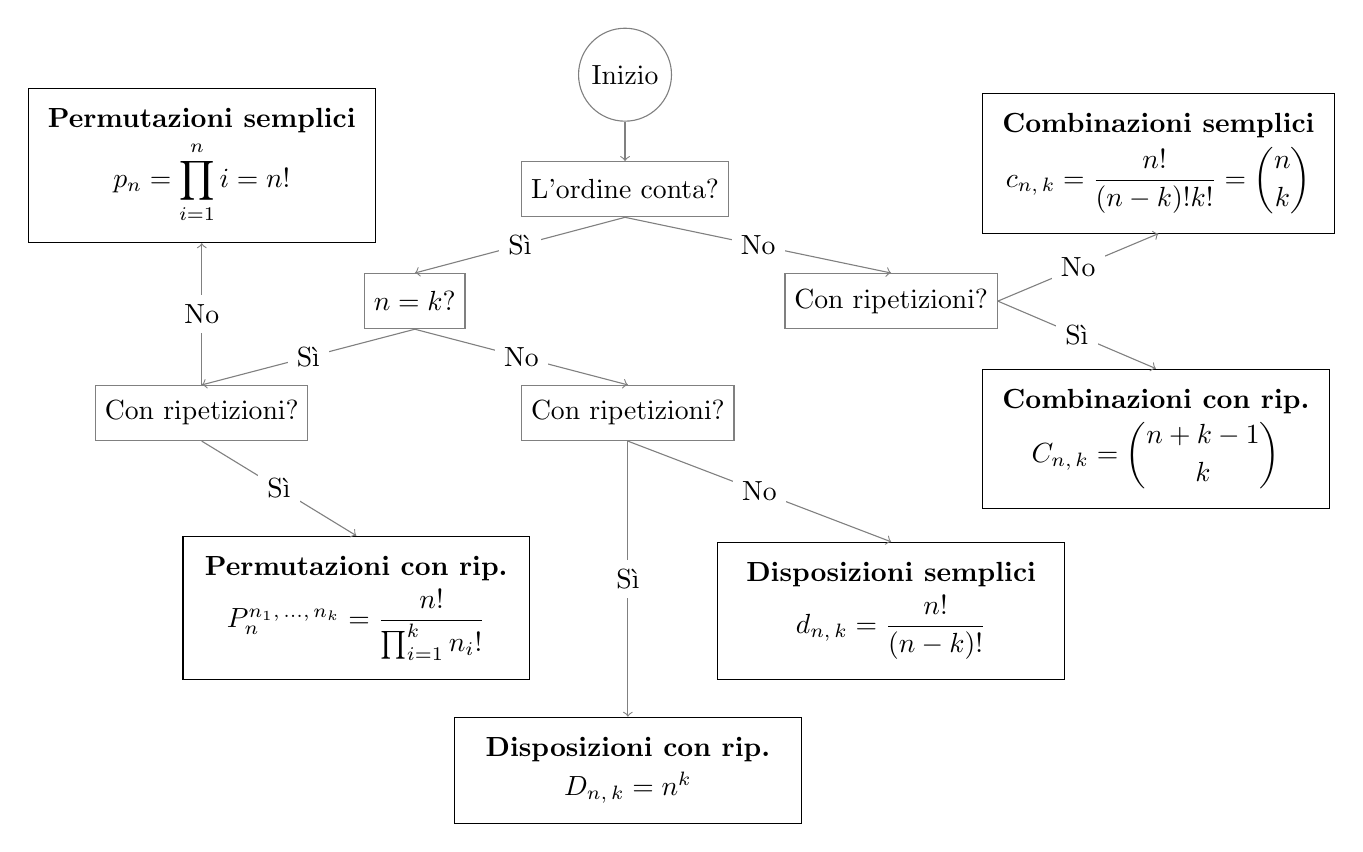
\begin{tikzpicture}[
round/.style={circle, draw=gray, minimum size=10mm},
rect/.style={rectangle, draw=gray, minimum size=7mm},
bigrect/.style={rectangle, draw=black, minimum width=4.4cm, inner sep=2.5mm},
]

\node[round] (start) {Inizio};
\node[rect] (order) [below=5mm of start] {L'ordine conta?};
\node[rect] (nk) [below left=10mm of order] {$n=k$?};
\node[rect] (rip1) [below right=10mm of order] {Con ripetizioni?};

\node[rect] (rip2) [below left=10mm of nk] {Con ripetizioni?};
\node[bigrect] (perm_s) [above=18mm of rip2, align=center] {\textbf{Permutazioni semplici} \\[0.8mm]
$p_n = \displaystyle \prod_{i=1}^n i = n!$
};
\node[bigrect] (perm_r) [below right=12mm and -16mm of rip2, align=center] {\textbf{Permutazioni con rip.} \\[0.8mm]
$P_n^{n_1, \, \dots, \, n_k} = \displaystyle \frac {n!}{\prod_{i=1}^k n_i!}$
};

\node[bigrect] (comb_s) [above right=5mm and -2mm of rip1, align=center] {\textbf{Combinazioni semplici} \\[0.8mm]
$c_{n, \, k} = \dfrac{n!}{(n-k)!k!} = \displaystyle \binom{n}{k}$
};
\node[bigrect] (comb_r) [below right=5mm and -2mm of rip1, align=center] {\textbf{Combinazioni con rip.} \\[0.8mm]
$C_{n, \, k} = \displaystyle \binom{n+k-1}{k}$
};
\node[rect] (rip3) [below right=10mm of nk] {Con ripetizioni?};
\node[bigrect] (disp_s) [below=27mm of rip1, align=center] {\textbf{Disposizioni semplici} \\[0.8mm]
$d_{n, \, k} = \dfrac{n!}{(n-k)!}$
};
\node[bigrect] (disp_r) [below=35mm of rip3, align=center] {\textbf{Disposizioni con rip.} \\[0.8mm]
$D_{n, \, k} = n^k$
};

\draw[gray, ->] (start.south) -- (order.north);
\draw[gray, ->] (order.south) -- (nk.north) node[black, midway, fill=white] {Sì};
\draw[gray, ->] (order.south) -- (rip1.north) node[black, midway, fill=white] {No};

\draw[gray, ->] (rip2.north) -- (perm_s.south) node[black, midway, fill=white] {No};
\draw[gray, ->] (rip2.south) -- (perm_r.north) node[black, midway, fill=white] {Sì};

\draw[gray, ->] (nk.south) -- (rip2.north) node[black, midway, fill=white] {Sì};
\draw[gray, ->] (nk.south) -- (rip3.north) node[black, midway, fill=white] {No};

\draw[gray, ->] (rip3.south) -- (disp_r.north) node[black, midway, fill=white] {Sì};
\draw[gray, ->] (rip3.south) -- (disp_s.north) node[black, midway, fill=white] {No};

\draw[gray, ->] (rip1.east) -- (comb_s.south) node[black, midway, fill=white] {No};
\draw[gray, ->] (rip1.east) -- (comb_r.north) node[black, midway, fill=white] {Sì};
\end{tikzpicture}
\end{figure}


\subsection{Definizioni}
Iniziamo con un po' di definizioni informali: \begin{itemize}
    \item un \textbf{evento} è la descrizione delle \textit{cose} che possono (o no) succedere come esito di un \textit{esperimento}. Per esempio, dato l'esperimento di un lancio di dadi, un evento può essere ``\textit{esce 4}" o ``\textit{esce un numero pari}";
    \item un \textbf{esito} di un esperimento può essere un intero o un risultato, mentre un evento è un insieme di esiti;
    \item la \textbf{probabilità} è la quantificazione dell'incertezza di un evento. 
\end{itemize}

\noindent Alla probabilità si possono dare numerose interpretazioni filosofiche, come: \begin{itemize}
    \item l'\textbf{interpretazione frequentista} utilizza la notazione della frequenza per definire la probabilità come il $\lim_{\text{\# prove} \rightarrow +\infty} f'(I)$;
    \item l'\textbf{interpretazione soggettivista} è la misura del grado di fiducia che un individuo coerente attribuisce, secondo le sue informazioni e opinioni, all'avverarsi di un evento $E$. 
\end{itemize}

\noindent Per studiare la probabilità utilizziamo invece un \textbf{approccio matematico/assiomatico}, ignorando i problemi filosofici relativi all'interpretazione di essa.
Con gli strumenti matematici che abbiamo a disposizione (in particolare la notazione sistemistica), tentiamo di formalizzare i concetti di evento, esperimento casuale, ecc.

\subsubsection{Spazio campionario}
Iniziamo con il concetto di {spazio campionario} (o \textit{insieme degli esiti} o \textit{insieme universo)}, annotato con $\Omega$. 
Lo spazio campionario può essere \textbf{finito} (come il sesso di un nascituro, $\Omega = \{ \text{F}, \, \text{M} \}$ o l'esito di una corsa di 7 cavalli $\Omega = \{ \text{permutazioni di 7 oggetti} \}$ $|\Omega| = 7!$) o \textbf{infinito} (come il dosaggio minimo di un farmaco, $\Omega = \mathbb{R}^+$). Questi insiemi sono \textbf{continui o discreti}, e non gli elementi contenuti all'interno. \\ Un particolare \textbf{esito} dell'insieme viene indicato con $\omega \in \Omega$.


\subsubsection{Evento} 
Un evento è un sottoinsieme dello spazio campionario $E \subseteq \Omega$ e può quindi comprendere più esiti. \\ Un evento formato da un solo esito $\{ \omega \}$ si dice \textbf{evento elementare}.
Se $E = \Omega$ allora l'evento ha \textbf{probabilità certa}, mentre se $E = \varnothing$ allora è \textbf{impossibile}.

\noindent Dati due eventi è possibile applicare le operazioni fondamentali degli insiemi: \begin{itemize}
    \item $E \cup F$ è l'evento che si verifica se si verifica almeno uno dei due eventi \\ ($x \in E \cup F \Leftrightarrow x \in E \lor x \in F$ or non esclusivo);
    \item $E \cap F$ è l'evento che si verifica se si verificano entrambi gli eventi. \\ ($x \in E \cap F \Leftrightarrow x \in E \land x \in F$) \\ Se $E \cap F = \varnothing$ allora $E$ e $F$ si dicono \textbf{mutualmente esclusivi};
    \item $E^\mathtt{C} = \overline E$ è l'evento che si verifica se $E$ non si verifica \\ ($x \in \overline E \Leftrightarrow x \notin E $) inoltre $\overline E = \omega - E$ ;
    \item $E \subseteq F$ se $E$ si verifica, allora $F$ si verifica: $E \rightarrow F$;
    \item $E - F$ se $E$ si verifica, e $F$ non si verifica \\ ($x \in E \cup F \Leftrightarrow x \in E \land x \notin F$) \\ Questa operazione non è simmetrica, infatti $E - F \neq F - E$;
\end{itemize}

\noindent Inoltre, valgono le seguenti proprietà e notazioni (valgono sia per l'unione che per l'intersezione): \begin{itemize}
    \item $E \subseteq F \land F \subseteq E \Leftrightarrow E = F$;
    % \item $E_1 \cup E_2 \cup \dots \cup E_n = \displaystyle \bigcup_{i=1}^n E_i$ e $E_1 \cap E_2 \cap \dots \cap E_n = \displaystyle \bigcap_{i=1}^n E_i$;
    \item commutatività: $E \cup F = F \cup E$ \textit{(e viceversa)};
    \item associatività: $E \cup F \cup G = (E \cup F) \cup G = E \cup (F \cup G)$ \textit{(e viceversa)};
    \item distributività: $E \cup (F \cap G) = (E \cup F) \cap (E \cup G)$ \textit{(e viceversa)};
    \item leggi di De Morgan: $\overline{E \cup F} = \overline E \cap \overline F$ \textit{(e viceversa)}.
\end{itemize}

\begin{dimostrazione} dimostrazione legge di De Morgan $x \in (\overline{E \cup F}) \Leftrightarrow x \in (\overline{E} \cap \overline{F})$
\begin{align} 
    x \in \overline{E \cup F} \Leftrightarrow x \notin E \cup F \Leftrightarrow x \notin E \land x \notin F \\
    x \in \overline{E} \cap \overline{F} \Leftrightarrow x \in \overline{E} \land x \in \overline{F} \Leftrightarrow x \notin E \land x \notin F
\end{align}
\end{dimostrazione}



\subsubsection{Algebra di eventi} 
Una algebra di eventi $\mathcal{A}$ è un insieme di eventi $\{E_1, \, E_2, \, \dots\}$ che soddisfa le seguenti condizioni: \begin{itemize}
    \item $\boxed{\forall E \in \mathcal{A} \ \  E \subseteq \Omega}$, tutti gli eventi sono sottoinsieme di $\Omega$;
    \item $\boxed{\Omega \in \mathcal{A}}$, $\Omega$ stessa è inclusa nell'algebra; 
    \item $\boxed{\forall E \in \mathcal{A} \ \  \overline E \in \mathcal{A}}$, per ogni evento $E$ appartenente all'algebra allora anche il relativo complementare appartiene all'algebra;
    \item $\boxed{\forall E, F \in \mathcal{A} \ \ E \cup F \in \mathcal{A}}$, per ogni coppia di eventi appartenenti all'algebra allora anche la loro \textit{unione} appartiene all'algebra. L'algebra è quindi chiusa rispetto all'operazione unione: \begin{itemize}
        \item per $|\Omega| < \infty$, allora $\forall E_1, E_2, \dots, E_n \in \mathcal{A} \ \ \bigcup_{i=1}^n E_i \in \mathcal{A}$;
        \item se la proprietà vale anche per $|\Omega| = \infty$, allora $\mathcal{A}$ si definisce \textit{$\sigma$-algebra}.
    \end{itemize}
\end{itemize}

\noindent È possibile dimostrare che $\mathcal{A}$ è chiusa anche rispetto all'operazione intersezione: complementando entrambi i membri dalla legge di De Morgan $\overline{E \cap F} = \overline E \cup \overline F$, si ricava che $\overline{\overline{E \cap F}} = \overline{\overline{E} \cup \overline{F}} \Rightarrow E \cap F = \overline{\overline E \cup \overline F}$. \\ \\
\noindent Se $|\Omega| < \infty$, allora $\mathcal{P}(\Omega) = \mathcal{A}$. L'algebra di eventi $\mathcal A$ è il \textit{dominio} della funzione di probabilità $P$. \\

\noindent Quando $\omega$ è finito, la maggior parte delle volte l'algebra degli eventi più banale e ovvia che si può considerare è \textbf{l'insieme delle parti di $\Omega$}

\subsubsection{Assiomi di Kolmogorov}
Fissato lo \textit{spazio misurabile} $(\Omega, \, \mathcal A)$, $P:\mathcal A \rightarrow \mathbb{R}$ è una \textit{funzione di probabilità} se e solo se: \begin{enumerate}
    \item $\boxed{\forall E \in \mathcal A \ \ 0 \leq P(E) \leq 1}$;
    \item $\boxed{P(\Omega) = 1}$;
    \item $\boxed{E \cap F = \varnothing \Rightarrow P(E \cup F) = P(E) + P(F)} \Rightarrow \smash{ \displaystyle \forall i, j \ i \neq j \ E_i \cap E_j = \varnothing \ \ P \! \left(\bigcup_{i=1}^n E_i \right) = \sum_{i=1}^n P(E_i)}$.
\end{enumerate}

\begin{teorema}
Dato uno spazio di probabilità $(\omega, \mathcal A, P )$
\[
\boxed{\forall E \in \mathcal A \ \ P(\overline E) = 1 - P(E)}
\]
\end{teorema}
\begin{dimostrazione}
\begin{align}
    E \cup \overline E = \Omega &\land E \cap \overline E = \varnothing \tag*{} \\
    P(E \cup \overline E) &= P(E) + P(\overline E) = P(\Omega) \tag{3° assioma di Kolmogorov} \\
    P(E) + P(\overline E) &= 1 \tag{2° assioma di Kolmogorov} \\
    P(\overline E) &= 1 - P(E) \tag*{$\blacksquare$}
\end{align} 
\end{dimostrazione}
\begin{corollario}
\[
\boxed{P(\varnothing) = 0}
\]
\end{corollario}
\begin{dimostrazione}
\begin{align}
    \overline \Omega &= \varnothing \tag*{} \\
    P(\Omega) &= 1 \tag{2° assioma di Kolmogorov} \\
    P(\overline \Omega) &= 1 - P(\Omega) = 0 \tag{teorema evento complementare} \\
    P(\varnothing) &= 0 \tag*{$\blacksquare$}
\end{align}
\end{dimostrazione}

\begin{teorema}
\[
\boxed{P(E \cup F) = P(E) + P(F) - P(E \cap F)}
\]
\end{teorema}

\pagebreak
\begin{dimostrazione}
Rappresentiamo graficamente gli insiemi $E$ ed $F$ e calcoliamo $\textnormal{I} \cap \textnormal{II} \cap \textnormal{III}$.

\begin{figure}[H]
    \vspace{\abovedisplayskip}
    \centering
    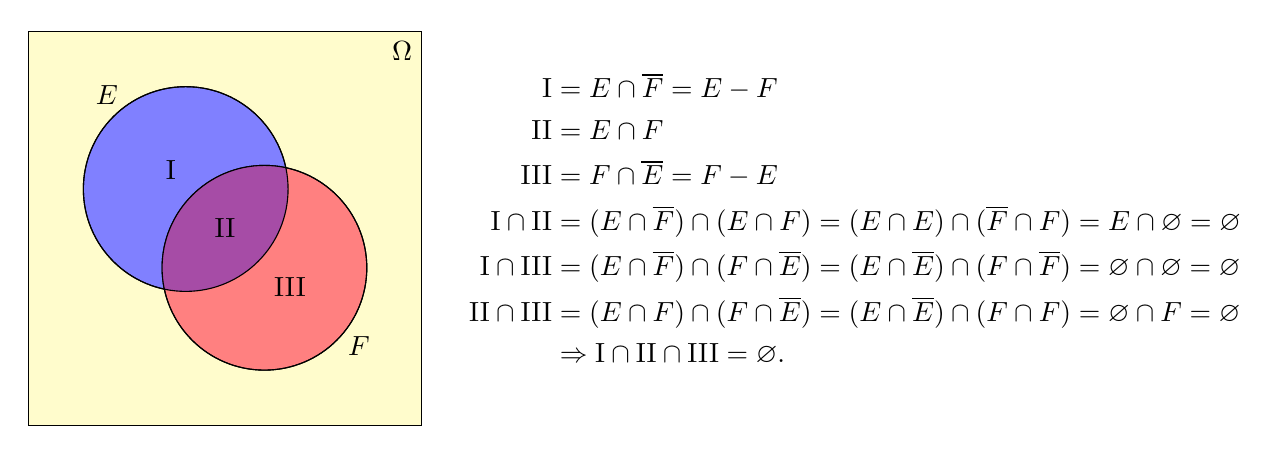
\begin{tikzpicture}
    \draw[fill=yellow!20] (0, 0) rectangle (5, 5) node [below left] {$\Omega$};
    \filldraw[black, fill=blue!50] (2, 3) circle (1.3) node [above left] {\textnormal{I}};
    \filldraw[black, fill=red!50] (3, 2) circle (1.3) node [below right] {\textnormal{III}};
    
    \begin{scope}
        \clip (2, 3) circle (1.3);
        \clip (3, 2) circle (1.3);
        
        \filldraw[violet!70](2.5, 2.5) circle(1.5cm);
    \end{scope}
    \node at (2.5, 2.5) {\textnormal{II}};
    
    \node at (1, 4.2) {$E$};
    \node at (4.2, 1) {$F$};
    
    \draw[black] (2, 3) circle (1.3);
    \draw[black] (3, 2) circle (1.3);
    
    \node[align=left, text width=10cm] at (10.5, 2.8) {\begin{align*}
        \textnormal{I} &= E \cap \overline F = E - F \\
        \textnormal{II} &= E \cap F \\
        \textnormal{III} &= F \cap \overline E = F - E \\
        \textnormal{I} \cap \textnormal{II} &= (E \cap \overline F) \cap (E \cap F) = (E \cap E) \cap (\overline F \cap F) = E \cap \varnothing = \varnothing \\
        \textnormal{I} \cap \textnormal{III} &= (E \cap \overline F) \cap (F \cap \overline E) = (E \cap \overline E) \cap (F \cap \overline F) = \varnothing \cap \varnothing = \varnothing \\
        \textnormal{II} \cap \textnormal{III} &= (E \cap F) \cap (F \cap \overline E) = (E \cap \overline E) \cap (F \cap F) = \varnothing \cap F = \varnothing \\
        &\Rightarrow \textnormal{I} \cap \textnormal{II} \cap \textnormal{III} = \varnothing.
    \end{align*}};
    \end{tikzpicture}
    \caption{Calcolo di I, II e III e relativa intersezione}
    \label{fig:omega}
    \vspace{\belowdisplayskip}
\end{figure}

\noindent Graficamente osserviamo che:
\[
P(E \cup F) = P(\textnormal{I} \cup \textnormal{II} \cup \textnormal{III}).
\]

\noindent Avendo dimostrato che $\textnormal{I} \cap \textnormal{II} \cap \textnormal{III} = \varnothing$, possiamo applicare il terzo assioma di Kolmogorov: \begin{align*}
P(\textnormal{I} \cup \textnormal{II} \cup \textnormal{III}) &=
\overbrace{
P(\textnormal{I}) + P(\textnormal{II})}^{=P(E)} + \,
\overbrace{ P(\textnormal{III}) \green{\, + \, P(\textnormal{II})}}^{=P(F)} % SHITTY HACKS IT WORKS DON'T TOUCH
\red{\, - \,} \overbrace{\red{P(\textnormal{II})}}^\text{\makebox[0pt]{$=\! \! P(E \cap F)$}} \\
&= P(E) + P(F) - P(E \cap F) \tag*{$\blacksquare$}
\end{align*}
\end{dimostrazione}

\subsubsection{Spazio di probabilità}
Uno spazio di probabilità è definito come una tripla $(\Omega, \, \mathcal A, \, P)$.

\paragraph{Spazio di probabilità equiprobabile} 
Nello spazio di probabilità equiprobabile tutti i casi $\omega \in \Omega$ hanno la stessa probabilità. Più precisamente, dato uno spazio campionario $\Omega = \{\mathit 1, \, \mathit 2, \, \dots, \, N \}$, $\forall \omega \in \Omega \ \ P(\{ \omega \}) = p$.
È possibile calcolare il valore di $p$ utilizzando il secondo assioma di Kolmogorov:
\[
P(\Omega) = 1 = \sum_{i=1}^N P(\{ \omega_i \}) = \sum_{i=1}^N p = Np \Rightarrow p = \frac{1}{N}.
\]
Non è possibile essere in uno spazio di probabilità equiprobabile se $|\Omega| = \infty$: se lo fosse allora $N = \infty$ e $p \rightarrow 0$. Ma se $\forall \omega \in \Omega \  \ P(\{ \omega \}) = 0$, allora gli assiomi di Kolmogorov non sono più soddisfatti, quindi $\perp$.


\subsection{Probabilità condizionata}
\label{subsec:probabilità_condizionata}
Consideriamo il lancio in sequenza di due dadi non truccati aventi 6 facce. Se il primo dado ha come esito $\mathit 3$, {qual è la probabilità} che la \textit{somma} data dall'esito del primo e del secondo dado sia $\mathit 8$?
Il problema appena citato è di probabilità condizionata, perché tentiamo di calcolare la probabilità di un evento $E$ (\textit{la somma dei due esiti \mbox{è 8}}) \textbf{limitatamente} ai casi in cui si verifica anche un altro evento $F$ (\textit{il primo esito è 3}); si indica con: \[
P(E|F).
\]

\noindent Utilizzando la notazione insiemistica, limitare i casi per cui l'evento $E$ si verifica equivale a ``\textit{ridefinire}" l'insieme $\Omega$ in $F$, quindi considerare l'intersezione $E \cap F$ (\figurename \ \ref{fig:prob_cond}).

\begin{figure}[h]
    \vspace{\abovedisplayskip}
    \centering
    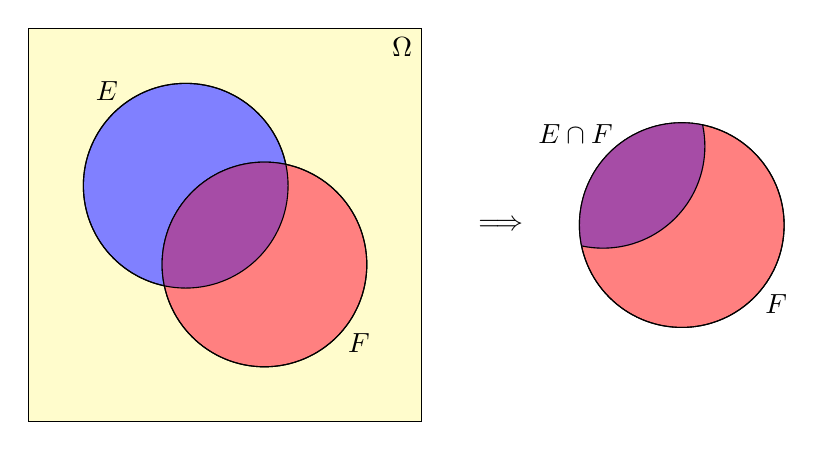
\begin{tikzpicture}
    \draw[fill=yellow!20] (0, 0) rectangle (5, 5) node [below left] {$\Omega$};
    \filldraw[black, fill=blue!50] (2, 3) circle (1.3);
    \filldraw[black, fill=red!50] (3, 2) circle (1.3);
    
    \begin{scope}
        \clip (2, 3) circle (1.3);
        \clip (3, 2) circle (1.3);
        \filldraw[violet!70](2.5, 2.5) circle(1.5cm);
    \end{scope}
    \node at (1, 4.2) {$E$};
    \node at (4.2, 1) {$F$};
    \draw[black] (2, 3) circle (1.3);
    \draw[black] (3, 2) circle (1.3);
    
    \node at (6, 2.5) {$\Longrightarrow$};
    
    %\filldraw[black, fill=blue!50] (7.3, 3.5) circle (1.3);
    \filldraw[black, fill=red!50] (8.3, 2.5) circle (1.3);
    \begin{scope}[even odd rule]
        \clip (7.3, 3.5) circle (1.3);
        \clip (8.3, 2.5) circle (1.3);
        \filldraw[violet!70](7.8, 3) circle(1.5cm);
        \draw[black, thick] (7.3, 3.5) circle (1.3);
    \end{scope}
    
    \node at (6.95, 3.65) {$E \cap F$};
    \node at (9.5, 1.5) {$F$};
    \draw[black] (8.3, 2.5) circle (1.3);
    \end{tikzpicture}
    
    \caption{Trasformazione dello spazio campionario $\Omega$ in $F$}
    \label{fig:prob_cond}
    
    \vspace{\belowdisplayskip}
\end{figure}

\noindent Utilizzando la definizione classica di probabilità ($P=\frac{\text{\# casi favorevoli}}{\text{\# casi possibili}} = \frac{|E|}{|\Omega|}$), possiamo ricavare la seguente formula risolutiva: \[
\boxed{P(E|F) = \frac{P(E \cap F)}{P(F)}}.
\]
Se $F = \varnothing$ quindi $P(F) = 0$ allora $P(E|F)$ si dice \textbf{indefinita}.

\subsubsection{Teorema delle probabilità totali}
Evidenziando $P(E \cap F)$ nella formula precedente, è possibile ricavarlo avendo a disposizione gli altri due dati: \[
P(E \cap F) = P(F) \cdot P(E|F).
\]
Questo lemma chiamato \textbf{regola di fattorizzazione} è molto utile per risolvere problemi dove è nota la probabilità condizionata ma non $E \cap F$. Possiamo invece ricavare $P(E)$ con il seguente teorema:

\begin{teorema}[Teorema delle probabilità totali]
Dati due eventi $E, \, F \in \mathcal A$, allora \[
\boxed{P(E) = P(E|F) \cdot P(F) + P(E|\overline F) \cdot P(\overline F)}.
\]
\end{teorema}
\begin{dimostrazione}
Come precedentemente mostrato in \figurename \ \ref{fig:omega}, siamo interessati a rappresentare $E$ come $\textnormal{I} \cup \textnormal{II}$, quindi come $(E \cap \overline F) \cup (E \cap F)$:
\[
    (E \cap \overline F) \cup (E \cap F) =
    E \cap (\overline F \cup F)
    = E \cap \Omega = E \tag{distributività}
\]
Per successivamente applicare il 3° assioma di Kolmogorov, è necessario mostrare che i due insiemi sono disgiunti: \[
 (E \cap \overline F) \cap (E \cap F) =
 (E \cap E) \cap (F \cap \overline F) = E \cap \varnothing = \varnothing.
\]

\noindent Scriviamo l'uguaglianza in funzione della probabilità \[
P(E) = P[(E \cap F) \cup (E \cap \overline F)]
\]
e applichiamo il 3° assioma di Kolmogorov: \[
P(E) = P(E \cap F) + P(E \cap \overline F).
\]
Dal primo lemma ricaviamo inoltre che $P(E \cap \overline F) = P(E | \overline F) \cdot P(\overline F)$, quindi: \begin{align*}
P(E) = P(E|F) \cdot P(F) + P(E|\overline F) \cdot P(\overline F) \tag*{$\blacksquare$}
\end{align*}
\end{dimostrazione}

\noindent È possibile estendere il teorema delle probabilità totali per un numero arbitrario di \textit{condizioni} $F_i$.

\begin{corollario}
Dato $F_{1, \dots, n}$ l'\textnormal{insieme partizione} di $\Omega$ ($\bigcup_{i=1}^n F_i = \Omega \land \forall i \neq j \ F_i \cap F_j = \varnothing$), allora: \[
\boxed{
P(E) = \sum_{i=1}^n P(E | F_i) \cdot P(F_i)
}
\]
\end{corollario}
\begin{dimostrazione}
Sapendo che $E \subseteq \Omega$, allora \[
\bigcup_{i=1}^n (E \cap F_i) = E \cap \bigcup_{i=1}^n F_i = E \cap \Omega = E.
\]
Naturalmente, l'intersezione è l'insieme vuoto: \[ 
\bigcap_{i=1}^n (E \cap F_i) = E \cap \bigcap_{i=1}^n F_i = E \cap \varnothing = \varnothing.
\]
Applicando il 3° assioma di Kolmogorov, ricaviamo che: \begin{align*}
    P(E) &= P\left(\bigcup_{i=1}^n (E \cap F_i) \right) = \\
    &= P[(E \cap F_1) \cup (E \cap F_2) \cup \dots \cup (E \cap F_n)] = \\
    &= P(E \cap F_1) + P(E \cap F_2) + \dots + P(E \cap F_n) = \\
    &= \sum_{i=1}^n P(E \cap F_i) = \sum_{i=1}^n P(E | F_i) \cdot P(F_i) \tag*{$\blacksquare$}
\end{align*}
\end{dimostrazione}

\subsection{Teorema di Bayes}
Fino ad ora ci siamo occupati della probabilità di un evento $E$ dato un evento $F$; vogliamo ora conoscere la probabilità che dato un evento $E$ accada $F$. È possibile ricavarla dalle altre probabilità utilizzando il teorema (o la formula) di Bayes:
$$
\boxed{
    P(F|E) = \frac{P(E|F) \cdot P(F)}{P(E)} 
}.
$$

$$= \frac{P(E|F) \cdot P(F)}{P(E|F) \cdot P(F) + P(E|\overline{F}) \cdot P(\overline{F})}
$$
Come per il teorema elle probabilità totali, si può estendere la formula di Bayes usando una partizione $F_1, \, \dots \, , F_n \subseteq \Omega$ (con $\forall i \: P(F_i) \neq 0$):
$$
P(F_j|E) = \frac{P(E|F_j) \cdot P(F_j)}{\sum_i{P(E|F_i) \cdot P(F_i)}}.
$$

\subsubsection{Classificatori \textit{naive}-Bayes}
Immaginiamo di dover calcolare la probabilità che un supereroe sia di una certa \textbf{casa produttrice} date due caratteristiche fisiche $x$ e $y$ (come il colore dei capelli o la forza).
Indichiamo con $P(M)$ la probabilità che l'eroe sia Marvel, e $P(X=x)$ (o $P(Y=y)$) che la caratteristica $X$ (o $Y$) abbia valore $x$ (o $y$). 
La probabilità che, dato un supereroe di caratteristiche $x$ e $y$ \textit{allora} il supereroe è Marvel la si può calcolare con Bayes:
\[ 
P(M|X=x \wedge Y=y) = \frac{P(X=x \wedge Y=y | M) \cdot P(M)}{P(X=x \wedge Y=y)}.
\]

\noindent Il classificatore Naive Bayes fa un'\textbf{assunzione ingenua}, che permette però di semplificare molto i calcoli a livello computazionale: si assume infatti che $P(X=x \wedge Y=y | M) \cdot P(M) = P(X=x| M) \cdot P(Y=y|M) \cdot P(M)$:
$$
P(M|X=x \wedge Y=y) = \frac{P(X=x| M) \cdot P(Y=y|M) \cdot P(M)}{P(X=x \wedge Y=y)}.
$$
Con questa semplificazione riusciamo a ridurre il numero di casi studiati da $|X| \cdot |Y|$ a $|X| + |Y|$. Il \textbf{denominatore} rimane però problematico, in quanto contiene un $\land$, quindi $|X| \cdot |Y|$ casi. Per rimuoverlo, possiamo fare una \textbf{generalizzazione}: supponiamo che vi sono più di due classi su cui suddividere i supereroi e quindi vi sono diversi valori $\{e_1, \, \dots, \, e_n\}$ per l'editore, dove abbiamo $E = e_k$. Una volta osservato un supereroe, sarà necessario calcolare $P(E = e_k \mid X = x_i \land Y = y_j)$ per tutti i possibili $e_k$: il più alto ottenuto individuerà l'editore da associare al supereroe. È possibile semplificare il procedimento, notando che esso consiste nel determinare, al variare di $k$, il più alto tra i valori 

\begin{align*}
    P(E=e_k | X = x_i \wedge Y = y_j) &\approx \frac{P(X = x_i \mid E = e_k) P(Y = y_j \mid E = e_k) \cdot P(E=e_k)}{P(X = x_i \wedge Y = y_j)}
\end{align*}
Ora il denominatore è indipendente da $k$ e quindi la classificazione si può effettuare trovando il valore $k$ che massimizza la quantità
\begin{align*}
    \Aboxed{\arg {\max}_{k} \  P(X = x_i \mid E = e_k) P(Y = y_j \mid E = e_k) \cdot P(E=e_k)}
\end{align*}
Possiamo rendere il ragionamento più generale: abbiamo sempre la nostra classe di possibili editrici $E = e_k$ e generalizziamo con una serie di caratteristiche $X_1 = x_1, \, \dots , \, X_n = x_n$.
Vogliamo calcolare $P(E=e_k | X_1 = x_1 \land \, \cdots \, \land X_n = x_n)$.
Applicando il teorema di Bayes si ottiene:

\begin{align*}
    P(E=e_k | X_1 = x_1 \wedge \, \cdots \, \wedge X_n = x_n) &= \frac{P(X_1 = x_1 \wedge \, \cdots \, \wedge X_n = x_n | E=e_k) \cdot P(E=e_k)}{P(X_1 = x_1 \wedge \, \cdots \, \wedge X_n = x_n)}
    \intertext{applicando la semplificazione fatta prima al numeratore, otteniamo:}
    P(E=e_k | X_1 = x_1 \wedge \, \cdots \, \wedge X_n = x_n) &= \frac{\prod_i P(X_i = x_i | E=e_k) \cdot P(E=e_k)}{P(X_1 = x_1 \wedge \, \cdots \, \wedge X_n = x_n)}
    \intertext{volendo creare il miglior classificatore, vogliamo massimizzare questa probabilità:}
    P(E=e_k | X_1 = x_1 \wedge \, \cdots \, \wedge X_n = x_n) &= \arg {\max}_{k} \frac{\prod_i P(X_i = x_i | E=e_k) \cdot P(E=e_k)}{P(X_1 = x_1 \wedge \, \cdots \, \wedge X_n = x_n)}
    \intertext{ma il denominatore non dipende da $k$, quindi:}
    \Aboxed{P(E=e_k | X_1 = x_1 \wedge \, \cdots \, \wedge X_n = x_n) &= \arg {\max}_{k} {\prod}_i P(X_i = x_i | E=e_k) \cdot P(E=e_k)}
\end{align*}

\subsection{Eventi indipendenti}
Dati due eventi $E, \, F$, allora: \[
\boxed{
P(E \cap F) = P(E) \cdot P(F) \Leftrightarrow \textnormal{$E$ e $F$ sono indipendenti}
};
\]
vale inoltre l'indipendenza tra $E$ e $\overline{F}$.

\begin{dimostrazione}[Indipendenza tra $E$ e $\overline F$]
Siano $E \cap F$ e $E \cap \overline{F}$ due insiemi disgiunti, la loro unione è $E$.
Applicando il 3° assioma di Kolmogorov, \[
P((E \cap F) \cup (E \cap \overline{F}))
    = P(E \cap F) + P(E \cap \overline{F}),
\]
allora:
\begin{align*}
    P(E \cap \overline{F}) &= P(E) - P(E \cap F) = \\
    &= P(E) - P(E) \cdot P(F) = \\
    &= P(E) \cdot (1 - P(F)) = \\
    &= P(E) \cdot P(\overline{F}) \tag*{$\blacksquare$}
\end{align*}

% Applico terzo assioma, $P((E \cap F) \cup (E \cap \overline{F})) = P(E \cap F) + P(E \cap \overline{F})$, ma allora $P(E \cap \overline{F}) = P(E) - P(E \cap F) = P(E) - P(E) \cdot P(F) = P(E) \cdot (1 - P(F)) = P(E) \cdot P(\overline{F})$
\end{dimostrazione}

\noindent Si può \textbf{generalizzare} questa proprietà a 3 eventi $E,\,F,\,G$, controllando le indipendenze due a due. Inoltre: 
\[
\text{$E,\,F, \,G$ sono indipendenti} \Rightarrow \text{$E$ e $F \cup G$ sono indipendenti}.
\]

\begin{dimostrazione}[Indipendenza tra $E$ e $F \cup G$]
\begin{align*}
    P(E \cap (F \cup G)) &= P((E \cap F) \cup (E \cap G)) \tag{distributività} \\
    &= P(E \cap F) + P(E \cap G) - \underbrace{P((E \cap F) \cap (E \cap G))}_{P(E \cap F \cap G)} \tag{$P(E) + P(F) - P(E \cap F$)} \\ 
    &= P(E) \cdot P(F) + P(E) \cdot P(G) - P(E) \cdot P(F) \cdot P(G) \\ 
    &= P(E) \cdot (P(F) + P(G) - P(F) \cdot P(G)) \\ 
    &= P(E) \cdot (P(F) + P(G) - P(F \cap G)) \\ 
    &= P(E) \cdot P(F \cup G) \tag*{$\blacksquare$}
\end{align*}
\end{dimostrazione}

\noindent Si può ulteriormente generalizzare per $n$ eventi $E_1, \, \dots, \, E_n \subseteq \Omega$ indipendenti: se $1 \leq \alpha_1 < \alpha_2 < \dots < \alpha_r \leq n$,
(Questo significa che per ogni modo in cui posso scegliere $\alpha$ valori differenti che vanno da $1$ a $r$, questa uguaglianza vale ($r$ al massimo uguale a $n$))
allora:
\[
P \left (\bigcap_{i=1}^r E{\alpha_i} \right ) = \prod_{i=1}^r P(E{\alpha_i})
\]



\subsection{Variabili aleatorie discrete}
Partendo da uno spazio di probabilità $(\Omega, \, \mathcal A, \, P)$, si definisce una \textbf{\textit{variabile aleatoria}} con dominio $X: \Omega \rightarrow \mathbb R$: \[
\boxed{
\{ X = \alpha \} \equiv \{ \omega \in \Omega : X(\omega) = \alpha \}
}.
\]
\noindent In base all'insieme dei valori \textit{``sensati"} ($\neq 0$) che assumono, possiamo \textbf{distinguere} le variabili aleatorie in \textbf{discrete} e \textbf{continue}. 
I valori assunti da una variabile aleatoria si chiamano \textbf{specificazioni} (o \textbf{realizzazioni}). 
In generale, indichiamo con $X$ la variabile aleatoria e con $x$ una sua particolare \textit{specificazione}.

\noindent Il dominio delle \textbf{variabili aleatorie discrete} è un insieme finito o infinito ma comunque \textbf{numerabile} di valori \[D_X = \{ x_1, \, x_2, \, \dots \},\]
dove $P(X = x_i) \neq 0$. Il supporto, o dominio, di una variabile aleatoria può essere calcolato trovando l'insieme di valori per cui la funzione di massa in corrispondenza di tale specificazione, non assuma valore nullo.

\subsubsection{Funzione di ripartizione}
Detta anche \textit{funzione di distribuzione cumulativa} (CDF), la funzione di ripartizione $F_X: \mathbb{R} \rightarrow [0,1]$ di una variabile aleatoria $X$ si definisce come
\[
\boxed{F_X(x) = P(X \leq x)}.
\]
Vediamo alcune delle sue proprietà per i modelli discreti:
\begin{itemize}
    \item assume valore $0$ quando $\lim\limits_{x \rightarrow +0} F_X = 0$ mentre assume valore $1$ quando $\lim\limits_{x \rightarrow +\infty} F_X = 1$;
    \item è una funzione \textbf{monotona non decrescente} e \textbf{continua a destra}, il che significa che se $x_1 < x_2$, allora $F(x_1) \leq F(x_2)$ e quindi non diminuisce mai con l'aumento di $x$;
    \item è una funzione a gradino che ha punti di discontinuità (salti) nei valori possibili della variabile. Questi punti di discontinuità corrispondono ai punti in cui la variabile aleatoria può assumere un nuovo valore;
    \item la probabilità che la variabile aleatoria assuma un valore compreso tra due punti $a$ e $b$ può essere calcolata come $P(a < X \leq b) = F_X(b) - F_X(a)$;
    \item è la somma delle probabilità $P(X \leq x)$ per tutti i valori di $X$ che sono minori o uguali a $x$;
\end{itemize}

\subsubsection{Funzione di {massa di probabilità}}
La funzione di massa di probabilità $p_X : \mathbb R \rightarrow [ 0, 1 ]$ si definisce nell'ambito delle variabili aleatorie discrete come \[
\boxed{p_X(x) = P(X = x)}.
\] ed indica la \textbf{probabilità} che la variabile aleatoria $X$ assuma una \textbf{particolare specificazione}. Ha le seguenti proprietà: \begin{itemize}
    \item $x \in \mathbb R \land x \notin D_X \Rightarrow p_X(x) = 0$: se $x$ non è nel dominio della variabile aleatoria allora ha \textbf{probabilità 0};
    \item $\forall x \in \mathbb R \ \  p_X(x) \geq 0$: la funzione è sempre \textbf{non negativa};
    \item $\sum_{x \in D_X} p_X(x) = P\left( \bigcup_{x \in D_X} \{ X = x \} \right) = P(\Omega) = 1$: tutti gli eventi sono \textbf{disgiunti} e la loro somma è $\Omega$.
\end{itemize}

\noindent È possibile scrivere la funzione di ripartizione in termini di massa di probabilità: \[
F_X(x) = P(X \leq x) = P\biggl(\bigcup_{\alpha \leq x} \{ X = \alpha \}\biggr) = \sum_{\alpha \leq x} P(X = \alpha) = \sum_{\alpha \leq x} p_X (\alpha).
\]
Viceversa, è inoltre possibile scrivere la massa di probabilità in termini di funzione di ripartizione: \[
p_X (x) = P(X = x) = P(x' < X \leq x) = F_X(x) - F_X(x').
\]

\begin{figure}[h]
    \centering
\subfloat[Funzione di massa di probabilità]{
    \resizebox{7cm}{!}{
        \begin{tikzpicture}
        \begin{axis}[
            clip=false,
            enlargelimits=false,
            axis lines = center,
            %axis equal,
            xlabel = $x$,
            ylabel = $p_X$,
            ymin=0, ymax=1.1,
            xmin=0, xmax=4,
            ytick = {1/6, 1/3, 0.5, 1},
            yticklabels={$\dfrac 16$, $\dfrac 13$, $\dfrac 12$, 1},
            xtick={1, 2, 3},
        ]
        %\addplot[color=blue, thick]{x^2+2};
        \draw[gray] (1, 0) -- (1, 0.5);
        \node[blue, circle, fill, inner sep=2pt] at (1, 0.5) {};
        \draw[gray] (2, 0) -- (2, 1/3);
        \node[blue, circle, fill, inner sep=2pt] at (2, 1/3) {};        
        \draw[gray] (3, 0) -- (3, 1/6);
        \node[blue, circle, fill, inner sep=2pt] at (3, 1/6) {};
        
        \draw[blue, ultra thick, inner sep=2pt] (0, 0) -- (4, 0);
        \node[black, circle, draw=black, fill=white, inner sep=2pt] at (1, 0) {};
        \node[black, circle, draw=black, fill=white, inner sep=2pt] at (2, 0) {};
        \node[black, circle, draw=black, fill=white, inner sep=2pt] at (3, 0) {};
        \end{axis}
        
        \end{tikzpicture}
    }
}
\subfloat[Funzione di ripartizione]{
    \resizebox{7cm}{!}{
        \begin{tikzpicture}
        \begin{axis}[
            clip = false,
            enlargelimits=false,
            axis lines = center,
            %axis equal,
            xlabel = $x$,
            ylabel = $F_X$,
            ymin=0, ymax=1.1,
            xmin=0, xmax=4,
            ytick = {1/2, 5/6, 1},
            yticklabels={$\dfrac 12$, $\dfrac 56$, 1},
            xtick={1,2,3},
        ]
        \draw[gray] (1, 0) -- (1, 0.5);
        \node[blue, circle, fill, inner sep=2pt] at (1, 0.5) {};
        \draw[gray] (2, 0) -- (2, 5/6);
        \node[blue, circle, fill, inner sep=2pt] at (2, 5/6) {};
        \draw[gray] (3, 0) -- (3, 1);
        \node[blue, circle, fill, inner sep=2pt] at (3, 1) {}; 
        
        \draw[blue, ultra thick, inner sep=2pt] (0, 0) -- (1, 0);
        \node[black, circle, draw=black, fill=white, inner sep=2pt] at (1, 0) {};
        
        \draw[blue, ultra thick, inner sep=2pt] (1, 0.5) -- (2, 0.5);
        \node[black, circle, draw=black, fill=white, inner sep=2pt] at (2, 0.5) {};
        
        \draw[blue, ultra thick, inner sep=2pt] (2, 5/6) -- (3, 5/6);
        \node[black, circle, draw=black, fill=white, inner sep=2pt] at (3, 5/6) {};
        
        \draw[blue, ultra thick, inner sep=2pt] (3, 1) -- (4, 1);

        \end{axis}
        \end{tikzpicture}
    }
}
    \caption{Rappresentazione grafica della stessa variabile aleatoria $X$}
    \label{fig:mas_prob_rip}
\end{figure}

\subsubsection{Valore atteso}
Data $X$ una variabile aleatoria discreta, $D_X = \{ x_1, \, x_2, \, \dots \}$ il suo dominio e $p_X$ la funzione di massa di probabilità, il valore atteso di $X$ si definisce come: \[
\boxed{
\mathbb E(X) = \sum_{\smash{x \in D_X}} x \cdot p_X(x) = \sum_{x \in D_X} x \cdot P(X = x)}
\] 
ed equivale alla \textbf{media pesata} con la probabilità dei valori che può assumere $X$.
\begin{framed} 
\noindent Il valore atteso indica la \textbf{centralità} della variabile aleatoria, ovvero il \textbf{baricentro} intorno al quale, considerando sempre la probabilità di massa come peso, \textit{``oscillano"} tutti i dati.
\end{framed}
\noindent Il valore atteso è un \textbf{operatore lineare}.

\begin{dimostrazione}[$\mathbb{E}$ è un operatore lineare]
Dimostriamo che $\forall a, \, b \in \mathbb R$, $\mathbb E (Y) = a \mathbb E (X) + b$. \begin{align*}
    \mathbb E (Y) &= \mathbb E (aX + b) = \\
    &= {\sum}_y y \cdot P (Y = y) = \\
    &= {\sum}_x (a x + b) P(X = x) = \\
    &= {\sum}_x (a x P(X = x) + b P(X = x)) = \\
    &= a \cancelto{\mathbb{E}(X)}{{\sum}_x x P(X = x)} + b \cancelto{1}{{\sum}_{x} P(X = x)} = \\
    &= a \mathbb E (X) + b
    \tag*{$\blacksquare$}
\end{align*}
\end{dimostrazione}

\noindent Dalla dimostrazione precedente, si può evincere che: \begin{itemize}
    \item $a = 0 \Rightarrow \mathbb E (b) = b$: si può considerare $b \in \mathbb R$ come una \textit{variabile aleatoria degenere};
    \item $b = 0 \Rightarrow \mathbb E(aX) = a \mathbb E (X)$.
\end{itemize}

\noindent Esiste un altro termine per indicare il valore atteso (oltre a valore atteso e aspettazione), ovvero \textbf{momento n-esimo} della variabile aleatoria.
Questo termine fa riferimento alla seguente definizione: \[
\boxed{
\mathbb E(X^n) = \sum_{x} x^n \cdot p_X(x)}
\]

\noindent È possibile calcolare anche il valore atteso di una qualche funzione $g(X)$ della variabile aleatoria $X$ (di cui si conosce la distribuzione), infatti anche $g(X)$ è una variabile aleatoria che ha una sua distribuzione. Una volta ricavata 
(ovvero si conosce la sua funzione di massa di probabilità) è possibile definire il valore atteso di una funzione di variabile aleatoria in questo modo: \[
\boxed{
\mathbb E(g(X)) = \sum_{x} g(x) \cdot p_X(x) = \sum_{x} g(x) \cdot P(X = x)}
\]

\subsubsection{Varianza}
La varianza misura quanto i valori si concentrano intorno al valore atteso.
Data una variabile aleatoria $X$ e il suo valore atteso $\mu = \mathbb E(X)$, si definisce come varianza di $X$: \[
\boxed{\operatorname{Var}(X) =
\sigma(X) = \mathbb E \left((X - \mu)^2 \right)
}.
\]

\noindent Si può dimostrare inoltre la seguente proprietà: \[
\boxed{
\operatorname{Var}(X) = \mathbb{E}\left(X^2\right) - \mathbb{E}(X)^2
}.
\]

\begin{dimostrazione}
Vogliamo dimostrare che $\mathbb E \left((X - \mu)^2 \right) = \mathbb{E}\left(X^2\right) - (\mathbb{E}(X))^2$: \begin{align*}
\operatorname{Var}(X) &= \mathbb E \left((X - \mu)^2 \right) = \\
&= \mathbb E \left(X^2 - 2 \mu X + \mu ^2 \right) = \\
&= \mathbb E (X^2) - 2 \mu \mathbb E(X) + \mu^2 = \\
&= \mathbb E (X^2) - 2 \mu^2 + \mu^2 = \\
&= \mathbb E (X^2) - \mathbb E(X)^2 
\tag*{$\blacksquare$}
\end{align*}
\end{dimostrazione}

\paragraph{Funzione indicatrice e varianza} 
Consideriamo $A \in \mathcal{A}$ un particolare evento e $I_A$ la sua funzione indicatrice: \[
I_A = \begin{cases}
    1 & \text{se $A$ si verifica} \\
    0 & \text{se $A$ non si verifica},
\end{cases}
\]
allora $
\operatorname{Var}(I_A) = \mathbb E \left ( I_A ^ 2 \right ) - \mathbb E \left ( I_A \right )^2 = P(A) - P(A)^2 = P(A)(1 - P(A))
$.

\paragraph{Linearità}
La varianza non è un operatore lineare, infatti: \[
\boxed{
\operatorname{Var}(aX + b) = a^2 \operatorname{Var}(X)
}.
\]

\begin{dimostrazione}[$\sigma$ non è un operatore lineare]
\begin{align*}
    \operatorname{Var(aX + b)} &= \E \left( \left( Y - \E \left (Y \right ) \right)^2 \right) = \\
    &= \E \left ( \left(a X + \cancel{b} - a \E(X) - \cancel b \right )^2 \right) = \\
    &= \E \left ( (a (X - \E(X)))^2 \right ) = \\
    &= \E \left ( a^2 (X - \E(X))^2 \right ) = \\
    &= a^2 \E \left ( (X - \E(X))^2 \right ) = \\
    &= a^2 \operatorname{Var}(X) \neq \operatorname{Var}(X)
    \tag*{$\blacksquare$}
\end{align*}
\end{dimostrazione}

\noindent Se $a=0$ allora stiamo calcolando la varianza di una costante, e la sua varianza è $0$

\subsubsection{Deviazione standard}
Analogamente, possiamo definire la deviazione standard come
$$
\boxed{
\sigma_X = \sqrt{\operatorname{Var}(X)}
}.
$$

\noindent Anche la deviazione standard \textbf{non è un operatore lineare}:
$$
\sigma_{aX + b} = \sqrt{a^2 \operatorname{Var}(X)} = |a| \sigma_X
$$

\subsection{Variabili aleatorie multivariate}
Le variabili aleatorie specificate da numeri reali sono dette univariate, mentre quelle specificate da \textbf{vettori} sono dette multivariate.
Per semplicità, si può considerare la variabile aleatoria $n$-variata come una tupla contenente $n$ variabili aleatorie univariate. Quando $n=2$ si dice che la variabile aleatoria è \textbf{bivariata}.

\subsubsection{Funzione di ripartizione congiunta}
La funzione di ripartizione $F$ per le v.a.\ univariate può essere generalizzata per le v.a.\ multivariate.
% Definita nell'ambito delle variabili aleatorie multivariate, andiamo a considerare la funzione di ripartizione $F$ generalizzandola al numero di componenti del vettore che specifica la variabile aleatoria \\ 
Ad esempio, sia $A$ variabile aleatoria bivariata formata da $X$, $Y$ variabili aleatorie univariate discrete, allora:
$$
\boxed{
F_{X,Y}(x,\,y) = P(X \leq x \wedge Y \leq y)
}
$$
Calcolando il limite di questa funzione per una delle due componenti a $+\infty$ otteniamo:
\begin{align*}
\lim_{y \to +\infty} F_{X,Y}(x, \, y) &= 
\lim_{y \to +\infty} P(X \leq x \wedge Y \leq y) = \\ 
&= P(X \leq x) \cdot \cancelto{\Omega}{\lim_{y \to +\infty} P(Y \leq y)} = \\ 
&= P(X \leq x) = \\ 
&= F_X(x).
\end{align*}
Il risultato $F_X(x)$ prende il nome di \textbf{funzione di ripartizione marginale} di $X$. \\

\noindent È possibile generalizzare il concetto di funzione di ripartizione per $n$ variabili aleatorie $X_1, \, X_2, \, \dots, \, X_n$: \[
F_{X_1, X_2, \dots, X_N} = P(\{ X_1 \leq x_1, \, X_2 \leq x_2, \, \dots, \, X_n \leq x_n \})
\]

\subsubsection{Funzione di massa di probabilità congiunta}
In modo analogo si definisce la funzione di massa di probabilità congiunta di una variabile aleatoria multivariata; per semplicità, usando l'esempio precedente con $A$ v.a.\ bivariata formata da $X,Y$ v.a.\ univariate, allora
$$
p_{X,Y}(x, \, y) = P(X = x \wedge Y = y).
$$
Non potendo passare al limite, possiamo sommare tutte le funzioni di massa di probabilità congiunta:
\begin{align*}
{\sum}_x p_{X,Y}(x,\,y) &= {\sum}_x P(\{X = x\} \cap \{Y = y\}) = \\
&= P\left({\bigcup}_x \{X = x\} \cap \{Y = y\}\right);
\intertext{sapendo però che $\bigcup_x \{X = x\} \cap \{Y = y\} = \{Y = y\} \cap \cancelto{\Omega}{{\bigcup}_x \{X = x\}} = \{Y = y\}$, allora}
&= {\sum}_x p_{X,Y}(x,y) = \\ 
&= P\left({\bigcup}_x \{X = x\} \cap \{Y = y\}\right) = \\ &= P(\{Y = y\}) = \\
&= p_Y(y)
\end{align*}

\noindent Il risultato $p_Y(y)$ prende il nome di \textbf{funzione di massa di probabilità marginale} di $Y$. \\

\noindent È possibile \textbf{generalizzare} il concetto di funzione di massa di probabilità per \textbf{$n$ variabili aleatorie} $X_1, \, X_2, \, \dots, \, X_n$: \[
p_{X_1, X_2, \dots, X_N}(x_1, \, x_2, \, \dots, \, x_n) = P(\{ X_1 = x_1, \, X_2 = x_2, \, \dots, \, X_n = x_n \})
\] 

\subsubsection{Indipendenza}
Estendiamo il concetto di \textit{indipendenza} a due variabili aleatorie $X$ e $Y$:
\[
\boxed{
X \text{ e } Y \ \text{sono indipendenti} \Longleftrightarrow \forall A,B \subseteq \mathbb R \: \ X \in A \ \textnormal{e} \ Y \in B \ \textnormal{sono indipendenti}
}
\]

\noindent Si può dimostrare che $X$ e $Y$ sono indipendenti \textbf{se e solo se} valgono le seguenti fattorizzazioni: \begin{enumerate}
    \item $F_{X,Y}(x,\,y) = F_X(x) \cdot F_Y(y)$
    \item $p_{X,Y}(x,\,y) = p_X(x) \cdot p_Y(y)$
    \item $P(X \in A, \, Y \in B) = P(X \in A) \cdot P(X \in B)$
\end{enumerate}

\begin{dimostrazione}[$X$ e $Y$ sono indipendenti $\Rightarrow \forall x, y \: \ p_{X, Y} (x, \, y) = p_X(x) \cdot p_Y(y)$]

Dalle fattorizzazioni precedenti, sappiamo che se $X$ e $Y$ sono indipendenti allora vale la seguente proprietà:
\[
\forall A,B \subseteq \mathbb{R} \: \ P(X \in A, \, Y \in B) = P(X \in A) \cdot P(Y \in B).
\]

\noindent Fissati $x$ e $y$ e posti $A = \{x\}$ e $B = \{y\}$, abbiamo \begin{align*}
    p_{X,Y} &= P(X=x, \, Y=y) =
    %
    \intertext{ma scrivere $X=x$ (e $Y=y$) equivale a scrivere $X \in A$ (e $Y \in B$)}
    &= P(X \in A, \, Y \in B) =
    %
    \intertext{applicando quindi l'ipotesi}
    &= P(X \in A, \, Y \in B) = \\
    &= P(X \in A) \cdot P(Y \in B) =
    %
    \intertext{tornando indietro, scrivere $X \in A$ (e $Y \in B$) equivale a scrivere a $X = x$ (e $Y = y$)}
    &= P(X \in A) \cdot P(Y \in B) = \\
    &= P(X = x) \cdot P(Y = y) = \\
    &= p_X(x) \cdot p_Y(y)
    \tag*{$\blacksquare$}
\end{align*}
\end{dimostrazione}

\begin{dimostrazione}[$\forall x, y \: \ p_{X, Y} (x, \, y) = p_X(x) \cdot p_Y(y) \Rightarrow X$ e $Y$ sono indipendenti]
Fissati $A$ e $B$, applichiamo il 3° assioma di Kolmogorov:
\begin{align*}
    P(X \in A, \, Y \in B) &= \sum_{
    \begin{subarray}{l}
    {x \in A}\\{y \in B}
    \end{subarray}
    } p_{X,Y}(x, \, y) =
    \intertext{allora applicando l'ipotesi abbiamo}
    & = \sum_{x \in A} \sum_{y \in B} p_X(x) \cdot p_Y(y) = \\
    &= \sum_{x \in A} p_X(x) \cdot  
    \sum_{y \in B} p_Y(y) =
    \intertext{applicando ora il 3° assioma di Kolmogorov alle due sommatorie, otteniamo}
    &= P(X \in A, \, Y \in B) = \\
    &= P(X \in A) \cdot P(Y \in B) \Rightarrow \\
    &\Rightarrow \textnormal{$A$ e $B$ sono indipendenti}
    \tag*{$\blacksquare$}
\end{align*}
\end{dimostrazione}

\noindent È possibile \textbf{generalizzare} il concetto di funzione di indipendenza per \textbf{$n$ variabili aleatorie} $X_1, \, X_2, \, \dots, \, X_n$: 
\[
\boxed{
X_1, \, X_2, \, \dots, \, X_n \text{ sono indipendenti} \Longleftrightarrow \forall A_1, \, \dots, \, A_N \subseteq \mathbb{R} \: \ 
P \left( \bigcap_{i=1}^n X_i \in A_i \right ) = \prod_{i=1}^n P(X_i \in A_i)
}
\]


\subsubsection{Valore atteso}
È possibile calcolare il valore atteso in funzione di due variabili aleatorie:
\[
\boxed{\mathbb E(f(x, \, y)) = {\sum}_{x,y} f(x, \, y) \cdot p_{X,Y} (x, \, y)};
\]
Ad esempio, se consideriamo $f(x, \, y) = x + y$: \[
\boxed{\mathbb E(X + Y) = \mathbb E(X) + \mathbb E(Y)}.
\]

\begin{dimostrazione}[$\mathbb E{[}X + Y{]} = \mathbb E(X) + \mathbb E(Y)$]
\begin{align*}
    \E[X+Y] &= {\sum}_x {\sum}_y (x + y) \cdot p_{X,Y}(x, \, y) = \\
    &= {\sum}_x {\sum}_y [ x \cdot p_{X,Y}(x, \, y) + y \cdot p_{X, Y} (x, \, y) ] = \\
    &= {\sum}_x {\sum}_y x \cdot p_{X, Y} (x, \, y) + {\sum}_x {\sum}_y y \cdot p_{X, Y} (x, \, y) = \\
    &= {\sum}_x x \underbrace{{\sum}_y p_{X, Y} (x, \, y)}_{\textnormal{$p_X(x)$ marginale}} + {\sum}_y y \underbrace{{\sum}_x p_{X, Y} (x, \, y)}_{\textnormal{$p_Y(y)$ marginale}} = \\
    &= {\sum}_x x \cdot p_X (x) + {\sum}_y y \cdot p_Y (y) = \\
    &= \E(X) + \E(Y) \tag*{$\blacksquare$}
\end{align*}
\end{dimostrazione}

\noindent La \textbf{linearità} del valore atteso (solo nella somma e non nel prodotto) si estende a più variabili aleatorie: \[
\E(X + Y + Z) = \E[(X + Y) + Z] = \E(X + Y) + \E(Z) = \E(X) + \E(Y) + \E(Z);
\]

\noindent in generale: \[
\boxed{
\E \left ( \sum_{i=0}^n X_i \right ) = \sum_{i=0}^n \sumi{x_i}
}.
\]

\noindent inoltre è sempre possibile dire che il valore atteso della somma di variabili aleatorie è  uguale alla somma dei valori attesi di queste (indipendentemente dal fatto che vi sia indipendenza o no tra le v.a). \\

\noindent Un altro risultato è il seguente: \[
\text{$X$ e $Y$ sono indipendenti} \Rightarrow \mathbb{E}(XY) = \mathbb{E}(X) \mathbb{E}(Y)
\]

\noindent Questo implica inoltre che \textbf{\boxed{\operatorname{Cov}(X,\,Y) = 0}}, e di conseguenza che, se $X_1, ..., X_n$ sono indipendenti allora:

\[
\boxed{
\operatorname{var} \left ( \sum_{i=1}^n X_i \right ) = \sum_{i=1}^n \operatorname{var}(X_i)} 
\]

\begin{dimostrazione}[$X$ e $Y$ sono indipendenti $\Rightarrow \mathbb{E}(XY) = \mathbb{E}(X) \mathbb{E}(Y)$]
\begin{align*}
    \E(X Y) &= {\sum}_x {\sum}_y x y \cdot p_{X,Y} (x, \, y)
    \intertext{ma se $X$ e $Y$ sono indipendenti allora si può fattorizzare $p_{X,Y}$}
    &= {\sum}_x {\sum}_y xy \cdot p_X (x) \cdot p_Y (y) = \\
    &= {\sum}_x x p_X (x) \cdot {\sum}_y y p_Y (y) = \\
    &= \E(X) \E(Y) \tag*{$\blacksquare$}
\end{align*}
\end{dimostrazione}

\noindent Lo \textit{scostamento medio} di una variabile aleatoria $X$ rispetto a una grandezza $c$ sarà sempre maggiore o uguale rispetto allo scostamento medio della stessa variabile aleatoria rispetto al suo valore atteso $\mu = \E(X)$: \[
\boxed{
\E \left [ (X-c)^2 \right ] \geq \E \left[ (X-\mu)^2 \right]
}
\]

\begin{dimostrazione}[$
\E 
{[}
(X-c)^2 
{]}
\geq \E {[} (X-\mu)^2 {]}$]
\begin{align*}
\E \left( (X-c)^2 \right) &= \E \left[ (X-\mu + \mu-c)^2 \right] = \\
&= \E \left[ (X-\mu)^2 + 2(\mu-c)(X-\mu) + (\mu-c)^2 \right] = \\
\intertext{essendo $\E(X-\mu) = \E(X-\E(X)) = \E(X) - \E(\E(X)) = \mu - \mu = 0$, possiamo rimuovere un addendo:}
&= \E \left[ (X-\mu)^2 \right ] + \cancel{2(\mu-c) \E(X-\mu)} + \underbrace{(\mu-c)^2}_{\geq 0} \geq \E\left[(X-\mu)^2\right] \\
&= \E\left[(X-\mu)^2\right] + \E\left[(\mu-c)^2\right] \geq \E\left[(X-\mu)^2\right] \\
&= \E\left[(X-\cancel{\mu}+\cancel{\mu}-c)^2\right] \geq \E\left[(X-\mu)^2\right] \\
&= \E \left[(X-c)^2 \right] \geq \E\left[(X-\mu)^2 \right]
\tag*{$\blacksquare$}
\end{align*}
\end{dimostrazione}

\noindent Questo ci permette di affermare che il nel caso in cui si voglia predire con il minor errore possibile (in termini di minimizzazione dell'errore quadratico medio) il valore che verrà assunto da una variabile aleatoria, questo sarà la sua aspettazione.

\subsubsection{Varianza}
Se si vede $\operatorname{Var}(X+Y) = \operatorname{Var}(X) + \operatorname{Var}(Y) + \operatorname{Cov}(X,\,Y) + \operatorname{Cov}(Y,\,X)$ si può scrivere la varianza di $n$ variabili aleatorie in vari modi
\begin{align*}
\operatorname{Var}\left(\sumi X_i\right) &= \sumi\operatorname{Var}(X_i) + {\sum}_{i \neq j} \operatorname{Cov}(X_i, \, X_j) 
\\ &= \sumi\operatorname{Var}(X_i) + 2 {\sum}_{i < j} \operatorname{Cov}(X_i, \, X_j) \\ 
&= {\sum}_{i \neq j} \operatorname{Cov}(X_i, \, X_j).
\end{align*}
Interessante notare che se $X$ e $Y$ sono indipendenti allora \begin{align*}
    \operatorname{Var}(X-Y) &= \operatorname{Var}(X + (-Y)) \\ 
    &= \operatorname{Var}(X) + (-1)^2 \operatorname{Var}(Y) \\
    &= \operatorname{Var}(X) + \operatorname{Var}(Y).
\end{align*}
Situazione diversa invece quando le variabili aleatorie sono dipendenti: infatti
$$
\operatorname{Var}(X-Y) = \operatorname{Var}(X) + \operatorname{Var}(Y) + 2\operatorname{Cov}(X, Y) = \operatorname{Var}(X) + \operatorname{Var}(Y) - 2\operatorname{Cov}(X, Y).
$$

\subsubsection{Covarianza}
Si definisce covarianza di due variabili aleatorie $X$ e $Y$ come: \[
\boxed{
\operatorname{Cov}(X, \, Y) = \E[(X-\mu_X)(Y-\mu_Y)].
}
\]

\noindent Alternativamente, è possibile definire la covarianza come: \[
\boxed{\operatorname{Cov}(X, \, Y) = \E(X Y) - \E(X)\E(Y)}.
\]

\begin{dimostrazione}[$\E{[}(X-\mu_X)(Y-\mu_Y){]} = \E(X Y) - \E(X)\E(Y)$]
\begin{align*}
    \E[(X-\mu_X)(Y-\mu_Y)] &= \E[X Y - \mu_X Y - \mu_Y X + \mu_X \mu_Y] = \\
    &= \E(X Y) - \mu_X \E(Y) - \mu_Y \E(X) + \mu_X \mu_Y = \\
    &= \E(X Y) - \mu_X \mu_Y - \cancel{\mu_X \mu_Y} + \cancel{\mu_X \mu_Y} = \\
    &= \E(X Y) - \E(X) \E(Y) \tag*{$\blacksquare$}
\end{align*}
\end{dimostrazione}
\noindent Da questa formula è possibile dedurre alcune proprietà come la simmetria:
$$\operatorname{Cov}(X, \, Y) = \operatorname{Cov}(Y \, X)$$
\noindent e il fatto che la covarianza generalizza il concetto di varianza:
$$\operatorname{Cov}(X, \, X) = \operatorname{Var}(X)$$ \\
\noindent La covarianza non è un \textbf{operatore lineare} in quanto è insensibile alla traslazione ma si comporta bene con la scalatura: \[
\operatorname{Cov}(aX + b, \, Y) = a\operatorname{Cov}(X, \, Y)
\]

\begin{dimostrazione}[La covarianza non è un operatore lineare]
\begin{align*}
    \operatorname{Cov}(aX + b, \, Y) &= \E[(aX +\cancel{b} -a\mu_X -\cancel{b})(Y-\mu_Y)] = \\
    &= a \E[(X-\mu_X)(Y-\mu_Y)] = \\
    &= a \operatorname{Cov}(X, \, Y) \tag*{$\blacksquare$}
\end{align*}
\end{dimostrazione}

\noindent Questa ``linearità" la si ha quando ad una variabile aleatoria si somma un'altra variabile aleatoria
\begin{align*}
    \operatorname{Cov}(X+Y, \, Z) = \mathbb{E}[(X+Y - (\mu_X + \mu_Y)(Z - \mu_Z)] = \mathbb{E}[((X-\mu_X) + (Y - \mu_Y))(Z - \mu_Z)] = \\ = \mathbb{E}[(X - \mu_X)(Z - \mu_Z) + (Y - \mu_Y)(Z - \mu_Z)] = \mathbb{E}[(X - \mu_X)(Z - \mu_Z)] + \mathbb{E}[(Y - \mu_Y)(Z - \mu_Z)] = \\ = \operatorname{Cov}(X, \,Z) + \operatorname{Cov}(Y,\,Z).
\end{align*}

\noindent Per induzione si può dimostrare che
$$
\operatorname{Cov}\left(\sumi X_i, \, Z\right) = \sumi \operatorname{Cov}(X_i, \, Z).
$$
\noindent È possibile scrivere $\operatorname{Var}(X + Y)$ in funzione della covarianza:
\begin{align*}
    \operatorname{Var}(X+Y) &= \E\left[(X+Y)^2 \right] - \E(X+Y)^2 = \\
    &= \E\left[X^2+2X Y + Y^2\right] - (\E(X)+\E(Y))^2 = \\
    &= \E\left(X^2\right) + 2\E(X Y) + \E\left(Y^2\right) -\E(X)^2-2\E(X)\E(Y) -\E(Y)^2 = \\
    &= \underbrace{\E\left(X^2\right) - \E(X)^2}_{=\operatorname{Var}(X)} 
    + \underbrace{\E(Y^2)- \E(Y)^2}_{=\operatorname{Var}(Y)} + 2(\underbrace{\E(X Y) - \E(X)\E(Y)}_{=\operatorname{Cov}(X, \, Y)}) = \\
    &= \operatorname{Var}(X) + \operatorname{Var}(Y) + 2 \operatorname{Cov}(X, \, Y).
\end{align*}

 \noindent Un risultato ricavabile dalla formula appena enunciata è la seguente: \[
\boxed{
\operatorname{Cov}\left( \sum_{i=1}^n X_i, \, \sum_{j=1}^m Y_j\right) = \sum_{i=1}^n \sum_{j=1}^m \operatorname{Cov}(X_i, \, Y_j)
}.
\]

\begin{dimostrazione}[]
\begin{align*}
    \operatorname{Cov}\left( \sum_{i=1}^n X_i, \, \sum_{j=1}^m Y_j\right) &= \sum_{i=1}^n \operatorname{Cov}\left(X_i\sum_{j=1}^m Y_j\right) = \\
    &= \sum_{i=1}^n \operatorname{Cov}\left(\sum_{j=1}^m Y_j, \, X_i\right) = \\
    &= \sum_{i=1}^n \sum_{j=1}^m \operatorname{Cov}(X_i, \, Y_j)
    \tag*{$\blacksquare$}
\end{align*}
\end{dimostrazione}

\noindent Da notare come: \[
\operatorname{Var}(X+X) = \operatorname{Var}(X) + \operatorname{Var}(X) + 2 \operatorname{Cov}(X, \, X) = 4\operatorname{Var}(X).
\]

\noindent Inoltre: \[
\boxed{
X\text{ e } Y \text{ sono indipendenti} \Rightarrow \operatorname{Cov}(X, \, Y) = 0
}.
\]
\begin{dimostrazione}[$X\text{ e } Y \text{ sono indipendenti} \Rightarrow \operatorname{Cov}(X, \, Y) = 0$] Consideriamo la definizione di covarianza:
\begin{align*}
\operatorname{Cov}(X,\,Y) &= \mathbb{E}(X Y) - \mathbb{E}(X)\mathbb{E}(Y)
\intertext{ma se $X$ e $Y$ sono indipendenti allora si può fattorizzare il primo fattore, quindi}
&= \mathbb{E}(X)\mathbb{E}(Y) - \mathbb{E}(X)\mathbb{E}(Y) = 0
\tag*{$\blacksquare$}
\end{align*}
\end{dimostrazione}

\noindent Il precedente enunciato ha delle conseguenze anche sulla varianza: infatti, se $X$ e $Y$ sono indipendenti allora \[
\operatorname{Var}(X + Y) = \operatorname{Var}(X) + \operatorname{Var}(Y) + \cancelto{0}{2\operatorname{Cov}(X,Y)} = \operatorname{Var}(X) + \operatorname{Var}(Y).
\]

\noindent Se come nella la statistica descrittiva la covarianza indica la relazione tra due eventi, allora nel caso di indipendenza ha senso che non vi sia relazione, e che la covarianza sia 0. \\

\paragraph{\textbf{Esempio}}
Presentiamo ora un esempio per consolidare ciò che è stato detto. Consideriamo 10 variabili aleatorie $X_i$, ovvero $X_1, ..., X_{10}$, e diciamo che $X_i$ rappresenta l'esito \textbf{indipendente} del lancio di un dado non truccato. \\
Consideriamo ora una seconda variabile aleatoria $Y = \sum_{i=1}^{10} X_i$, ovvero la somma delle 10 variabili aleatorie. Possiamo dire che il valore atteso di $Y$ è $$Y = \mathbb{E}(Y) = \sumi{\mathbb{E}(X_i)}$$ Mentre la sua varianza è $$\operatorname{Var}(Y) = \operatorname{Var}(\sumi{X_i})$$ Siccome sappiamo che ogni lancio del dado è indipendente dagli altri possiamo dire che $$\operatorname{Var}(Y) = \operatorname{Var}(\sumi{X_i}) = \sumi{\operatorname{Var}(X_i)}$$
A questo punto ricordando che la varianza del lancio di un dado non truccato vale $\frac{35}{12} = \frac{36 - 1}{12}$ possiamo dire che $$\operatorname{Var}(Y) = \sumi{\operatorname{Var}(X_i)} = \sum_{i=1}^{10} \frac{35}{12} = \frac{35}{12} \cdot 10 = \frac{350}{12}$$
Tutto ciò è possibile dirlo partendo dal fatto che c'è indipendenza tra le $X_i$, ma se non ci fosse? ecco cosa si potrebbe dire. \\
Partiamo considerando $A, B \in \mathcal{A}$ e le loro due funzioni indicatrici $I_A \text{ e } I_B$, che sono a loro volta due variabili aleatorie che chiameremo rispettivamente $X \text{ e } Y$, quindi \[
\begin{array}{c}
X = I_A = \begin{cases}
    1 & \text{se $A$ si verifica} \\
    0 & \text{se $A$ non si verifica}
\end{cases} \,

Y = I_B = \begin{cases}
    1 & \text{se $B$ si verifica} \\
    0 & \text{se $B$ non si verifica}
\end{cases}
\end{array}
\]
A questo punto i valori attesi di $X \text{ e } Y$ saranno uguali rispettivamente alla probabilità di $A \text{ e di } B$.
$$\mathbb{E}(X) = 1 \cdot P(A) + 0 \cdot P(A) = P(A) = P(X = 1)$$
$$\mathbb{E}(Y) = 1 \cdot P(B) + 0 \cdot P(B) = P(B) = P(Y = 1)$$
E a questo punto, cosa possiamo dire di $X \cdot Y$? \\
Definiamo $X \cdot Y$ come \[
XY = I_A = \begin{cases}
    1 & \text{se $A$ e $B$ si verifica} \\
    0 & \text{altrimenti}
\end{cases}
\]
Quindi $$\mathbb{E}(XY) = 1 \cdot P(A \cap B) + 0 \cdot P(A \cap B) = P(A \cap B) = P(XY = 1)$$
Sfruttando la definizione alternativa di covarianza appena presentata, cerchiamo di ricavare la covarianza tra $X \text{ e } Y$: 

\begin{align*}
    \operatorname{Cov}(XY) = \mathbb{E}(XY) - (\mathbb{E}(X) \cdot \mathbb{E}(Y)) = P(XY = 1) - (P(X = 1) \cdot P(Y = 1)) 
\end{align*}

\noindent A questo punto abbiamo già dimostrato che se non c'è indipendenza $\operatorname{Cov} \neq 0$, quindo sarà o maggiore o minore di 0 (consideriamo $> 0$).

\begin{align*}
    \operatorname{Cov}(XY) = P(XY = 1) - (P(X = 1) \cdot P(Y = 1)) > 0 \\
    P(XY = 1) - (P(X = 1) \cdot P(Y = 1)) > 0 \\
    P(XY = 1) > (P(X = 1) \cdot P(Y = 1)) \\
     P(X = 1 \cap Y = 1) > (P(X = 1) \cdot P(Y = 1)) \\
    \intertext{Dividiamo tutto per }P(Y = 1) \\
    \frac{P(X = 1 \cap Y = 1)}{P(Y = 1)} > \frac{P(X = 1) \cdot P(Y = 1))}{P(Y = 1)} \\
    \frac{P(X = 1 \cap Y = 1)}{P(Y = 1)} > P(X = 1) \\
    \intertext{Ricordando \ref{subsec:probabilità_condizionata} possiamo dire che} \\
    P(X = 1 | Y = 1) > P(X = 1)
\end{align*}

\noindent Tutto ciò si può ricavare sapendo solo che $\operatorname{Cov} > 0$, di conseguenza sapendo che $Y$ assume valore $1$ aumenta la possibilità che $X = 1$. \\
Quindi all'aumentare dell'una possiamo dire che \textbf{tendenzialmente} anche l'altra variabile aleatoria aumenterà. Inoltre vi è simmetria, perché se avessimo diviso per $P(X = 1)$ il risultato sarebbe stato lo stesso ma invertendo $X \text{ e } Y$. \\
Nel caso in cui al posto del segno maggiore avessimo avuto il segno minore, si sarebbe ottenuto l'analogo della relazione indiretta tra le due variabili (all'aumentare del valore di $X$, quello di $y$ diminuisce). Da ciò si può concludere che la covarianza di una variabile aleatoria è l'analogo della varianza campionaria.

\subsubsection{Coefficiente di correlazione lineare}
Analogamente alla statistica descrittiva, è possibile definire il coefficiente di correlazione lineare dalla covarianza: \[
\boxed{
\rho_{X,Y} = \frac{\operatorname{Cov}(X, \, Y)}{\sigma_X \sigma_Y} = \frac{\operatorname{Cov}(X, \, Y)}{\sqrt{\operatorname{Var}(X)\operatorname{Var}(Y)}} 
}.
\]

\noindent Si può dimostrare che $-1 \leq \rho \leq +1$. Inoltre, $\rho$ è \textit{``immune"} alla scalatura: \[
\rho_{aX,bY} = \frac{\operatorname{Cov}(aX, \, bY)}{\sigma_{aX} \sigma_{bY}} = 
\frac{ab\operatorname{Cov}(X, \, Y)}{a\sigma_{X}b \sigma_{Y}} = \frac{\cancel{ab}\operatorname{Cov}(X, \, Y)}{\cancel{ab}\sigma_{X} \sigma_{Y}} = \rho_{X,Y}.
\]
Sapendo che $a, b > 0$ non è necessario mettere il valore assoluto al denominatore. \\
Due variabili aleatorie $X$ e $Y$ si dicono \textbf{indipendenti} se $\rho_{X,Y}=0$.
Questo concetto è del tutto analogo a quello del coefficiente di correlazione lineare descritto per la statistica descrittiva (\ref{sd:indice-correlazione-lineare})

\subsection{Variabili aleatorie continue}
Introduciamo il concetto di variabili aleatorie continue proponendo un metodo alternativo per calcolare il valore atteso: infatti, se $X \geq 0$ allora $\mathbb{E}(X) = \int\limits_0^{+\infty}{1 - F_X(x)} dx$. \\
Partiamo dal grafico della \textbf{funzione di ripartizione} di una v.a.\  discreta (\figurename \ \ref{fig:area_va_discreta}). Possiamo ricavare il valore atteso di $X$ dalla somma delle aree $\alpha$, $\beta$ e $\gamma$: \[
\E(X) = \alpha + \beta + \gamma = \int_0^{+\infty}{1 - F_X(x)} dx.
\]

\noindent Le variabili aleatorie continue sono delle variabili aleatorie che insistono su un dominio con cardinalità non numerabile, ad esempio l'insieme $\mathbb R$

\begin{figure}[h!]
    \vspace{\abovedisplayskip} 
    \centering
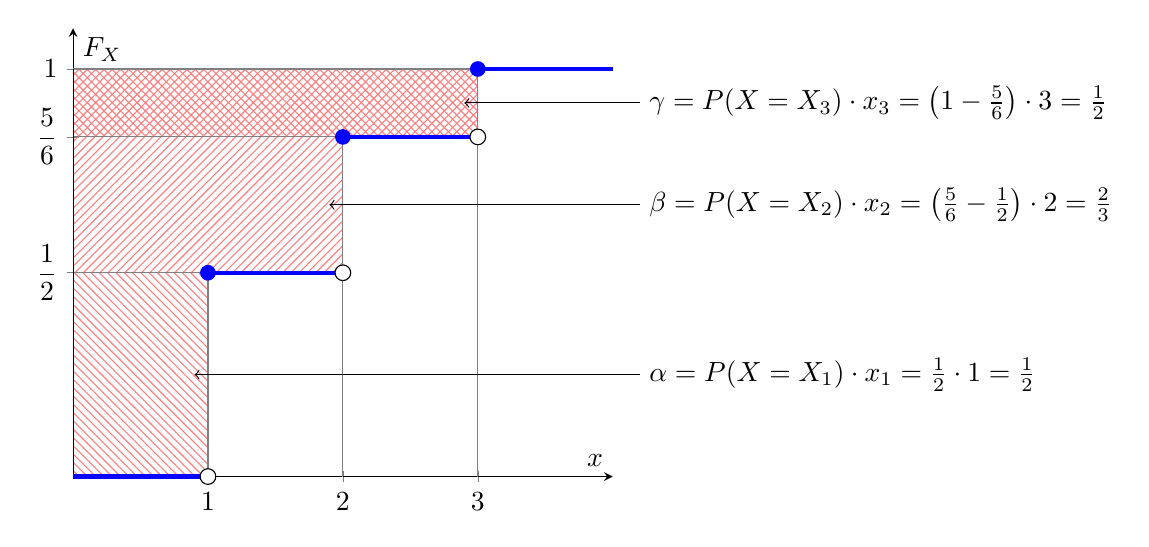
\begin{tikzpicture}
\begin{axis}[
    clip = false,
    enlargelimits=false,
    axis lines = center,
    %axis equal,
    xlabel = $x$,
    ylabel = $F_X$,
    ymin=0, ymax=1.1,
    xmin=0, xmax=4,
    ytick = {1/2, 5/6, 1},
    yticklabels={$\dfrac 12$, $\dfrac 56$, 1},
    xtick={1,2,3},
]
    \filldraw [draw=gray,pattern=north west lines, pattern color=red!50] (0, 0) rectangle (1, 1/2);
    \filldraw [draw=gray,pattern=north east lines, pattern color=red!50] (0, 1/2) rectangle (2, 5/6);
    \filldraw [draw=gray,pattern=crosshatch, pattern color=red!50] (0, 5/6) rectangle (3, 1);
    
    % overwrite overwritten axis
    \draw[black] (0, 0) -- (0, 1);
    
    \draw[gray] (1, 0) -- (1, 0.5);
    \node[blue, circle, fill, inner sep=2pt] at (1, 0.5) {};
    \draw[gray] (2, 0) -- (2, 5/6);
    \node[blue, circle, fill, inner sep=2pt] at (2, 5/6) {};
    \draw[gray] (3, 0) -- (3, 1);
    \node[blue, circle, fill, inner sep=2pt] at (3, 1) {}; 
    
    \draw[blue, ultra thick, inner sep=2pt] (0, 0) -- (1, 0);
    \node[black, circle, draw=black, fill=white, inner sep=2pt] at (1, 0) {};
    
    \draw[blue, ultra thick, inner sep=2pt] (1, 0.5) -- (2, 0.5);
    \node[black, circle, draw=black, fill=white, inner sep=2pt] at (2, 0.5) {};
    
    \draw[blue, ultra thick, inner sep=2pt] (2, 5/6) -- (3, 5/6);
    \node[black, circle, draw=black, fill=white, inner sep=2pt] at (3, 5/6) {};
    
    \draw[blue, ultra thick, inner sep=2pt] (3, 1) -- (4, 1);
    
    \draw[black, <-] (0.9, 1/4) -- (4.2,1/4) node[anchor=west] {$\alpha=P(X=X_1) \cdot x_1 = \frac 12 \cdot 1 = \frac 12$};
    \draw[black, <-] (1.9, 2/3) -- (4.2, 2/3) node[anchor=west] {$\beta=P(X=X_2) \cdot x_2 = \left( \frac 56 - \frac 12 \right) \cdot 2 = \frac 23$};
    \draw[black, <-] (2.9, 11/12) -- (4.2, 11/12) node[anchor=west] {$\gamma=P(X=X_3) \cdot x_3 = \left(1 - \frac 56\right) \cdot 3 = \frac 12$};
\end{axis}
\end{tikzpicture}
\caption{Calcolo del valore atteso dalla funzione di ripartizione di una variabile aleatoria discreta}
\label{fig:area_va_discreta}
\end{figure}

\subsubsection{Funzione di densità di probabilità}
Non si può più parlare di funzione di massa di probabilità, ma si deve introdurre la funzione di densità di probabilità $f_X : \mathbb R \rightarrow \mathbb R^+$ (quindi è una funzione non negativa); è definita come: \begin{gather*}
\boxed{
\forall B \subseteq \mathbb R \ \: P(X \in B) = \int_B f_X(x) dx}, \\
\text{con } \boxed{\int_{-\infty}^{+\infty} f_X(x) dx = P(X \in \mathbb R) = 1
}.
\end{gather*}

\noindent La probabilità viene quindi calcolata su un \textit{insieme di valori}, solitamente un intervallo: \[
P(a \leq X \leq b) = \int_a^b f_X(x) dx.
\]
\noindent Osserviamo come la probabilità di un particolare valore $x$ di $X$ non abbia molto senso: \[ 
P(X=a) = \int_a^a f_X(x) dx = 0;
\]
Per questo motivo i questo ambito non ci interessa che gli estremi siano inclusi o meno nella funzione di densità. \\
Un modo per approssimare questo valore è calcolare la probabilità per un intervallo molto piccolo (questo indica quanto è probabile che $X$ cada "vicino" ad a): \[
P\left(a - \frac \varepsilon 2 \leq X \leq a + \frac \varepsilon 2\right) = \int_{a-\frac \varepsilon 2}^{a + \frac \varepsilon 2} f_X (x) dx \approx \epsilon f_X(a) \approx f_X(a).
\]
\noindent Il motivo per cui non si può parlare di funzione di massa di probabilità per queste variabili aleatorie è che sono continue, quindi possono assumere un numero infinito di valori in un intervallo. Ricordiamo che la funzione di massa di probabilità rappresenta la probabilità che una variabile aleatoria assuma un valore specifico all'interno del suo dominio. Di conseguenza, se il dominio è infinito, la probabilità che la variabile assuma un qualsiasi valore specifico è estremamente bassa, tendente a zero. \\


\begin{figure}[h!]
    \vspace{\abovedisplayskip} 
    \centering
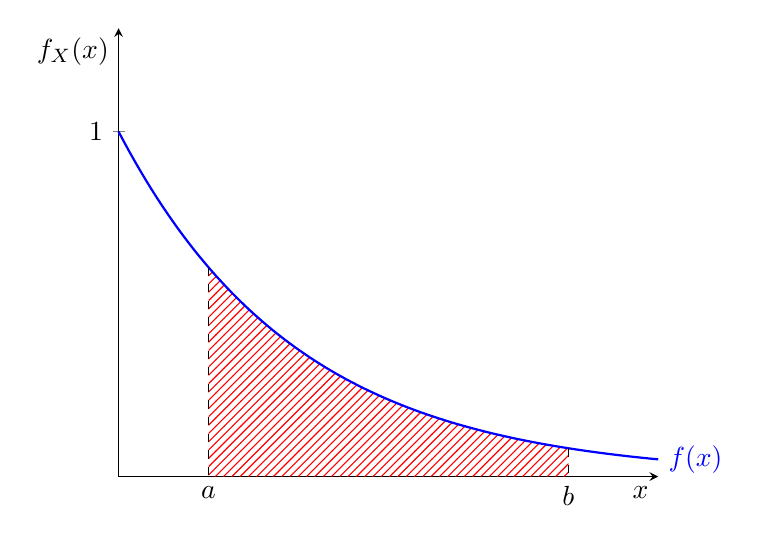
\begin{tikzpicture}
\begin{axis}[
    axis lines=middle,
    xlabel=$x$, ylabel=$f_X(x)$,
    xtick=\empty, ytick={1},
    xlabel style = {anchor=north east},
    ylabel style = {anchor=north east},
    ymin=0, ymax=1.3,
    xmin=0, xmax=3,
    clip=false,
    domain=0:3,
    samples=100]
\addplot [name path=A, domain=0:3, thick, blue] {exp(-x)} node[right] {$f(x)$};
\path [name path=B]
    (\pgfkeysvalueof{/pgfplots/xmin},0) --
    (\pgfkeysvalueof{/pgfplots/xmax},0);
\addplot [draw=none, pattern=north east lines, pattern color=red] 
    fill between [of=A and B, soft clip={(0.5,0) rectangle (2.5,5)},];
\draw[dashed]   (0.5,0.606) -- (0.5,0) node[below] {$a$}
                (2.5,0.082) -- (2.5,0) node[below] {$b$};
\end{axis}
\end{tikzpicture}
\caption{Esempio di funzione di densità di probabilità $f(x) = e^{-x} \textnormal{ per } x \geq 0$}
\label{fig:area_va_continua}
\end{figure}


\subsubsection{Funzione di ripartizione}
La funzione di ripartizione $F_X$ è anch'essa definita nel continuo: \[ 
\boxed{
F_X(x) = P (X \leq x) = \int_{-\infty}^x f_X(y) dy
}.
\]
La funzione di ripartizione è la \textbf{primitiva} della funzione di densità. Infatti, per il teorema fondamentale del calcolo integrale: \[
\frac { d F_X(x)}{dx} = f_X(x).
\]
Vediamo alcune delle sue proprietà per i modelli continui:
\begin{itemize}
    \item ha limiti quando l'argomento $x$ tende a $\pm \infty$:
    \begin{itemize}
        \item \textbf{Limite sinistro}: $F(x)$ tende a $0$ quando $x$ tende a meno infinito $\lim_{x \rightarrow -\infty} F(x) = 0$.
        \item \textbf{Limite destro}: $F(x)$ tende a $1$ quando $x$ tende a più infinito $\lim_{x \rightarrow +\infty} F(x) = 1$.
    \end{itemize}
    \item è una funzione \textbf{monotona non decrescente} e continua, senza salti o discontinuità. In altre parole, $F(x)$ è continua per tutti i valori di $x$ e non diminuisce mai con l'aumentare del valore.
    \item La probabilità che la variabile aleatoria assuma un valore compreso tra due valori $x_1$ e $x_2$ può essere calcolata come $P(x_1 \leq X \leq x_2) = F(x_2) - F(x_1)$.
\end{itemize}

\subsubsection{Altri indici}
È possibile ridefinire gli altri indici delle v.a.\ discrete per le v.a.\ continue integrando: \begin{align*}
\E(X) &= \int_{-\infty}^{+\infty} x f_X(x) dx
\\
E(g(x)) &= \int_{-\infty}^{+\infty} g(x) f_X(x) dx \\
\operatorname{Var}(X) = \E\left((X-\mu)^2\right) &= \int_{-\infty}^{+\infty} (X-\mu)^2 f_X(x) dx.
\end{align*}

\noindent Anche in questo caso non è detto che il valore atteso esista, inoltre  l'integrale nel calcolo del valore atteso per variabili continue è l'equivalente continuo della sommatoria per variabili discrete, adattato alla natura delle distribuzioni di probabilità (funzione di ripartizione) in questi due diversi contesti.

\subsubsection{Quantile applicato alle variabili aleatorie continue}
Il concetto di quantile può essere esteso anche nel contesto delle variabili aleatorie continue. Considerando ad esempio il concetto di mediana visto per la statistica descrittiva (abbiamo studiato che la mediana $m$ è il quantile di livello $q = 0.5$, in seguito daremo una spiegazioni migliore), e applicandolo alle variabili aleatorie continue, possiamo dire che la probabilità che la v.a. $X$ assuma valori minori o uguali a $m$ è uguale a 0.5, quindi:
$$P (X \leq m) = q = 0.5$$
Il caso appena descritto è la mediana nella variabile aleatoria continua $X$, più in generale possiamo dire che: \\
Sia $\chi_q$ il quantile di livello $q \in [0, 1]$ allora \[ 
F_X(\chi_q) = P (X \leq \chi_q) = q
\] \\
di conseguenza $\chi_q$ sarà uguale all'inversa di $F_X$, quindi: \\
$$\chi_q = F_X^{-1}(q)$$

\begin{figure}[h!]
    \vspace{\abovedisplayskip} 
    \centering
\begin{tikzpicture}
\begin{axis}[
    axis lines=middle,
    xlabel=$x$,
    ylabel=$F(x)$,
    xticklabels={,,},
    yticklabels={,,},
    enlargelimits,
    clip=false,
    domain=0:1,
    samples=101,
    ymin=0,
    ymax=1.1,
    ytick={0.7, 1},
]
\addplot+[no marks, thick, blue] {1 - exp(-x)} node[right] {};
\draw [red, dashed] (axis cs:0.7,0) -- (axis cs:0.7,{1-exp(-0.7)}) -- (axis cs:0,{1 - exp(-0.7)});
\node at (axis cs:0.7,-0.1) {$\chi_q$};
\node at (axis cs:-0.1,{1-exp(-0.7)}) {$q = F({\chi_q})\quad \;$};
\end{axis}
\end{tikzpicture}
\caption{Generalizzazione concetto di quantile per V.A continue}
\label{fig:quantile_va}
\end{figure}

\noindent Non sempre le funzioni sono invertibili, ma nel nostro caso la funzione di ripartizione è una funzione monotona continua, che tende a $1$, quindi si può invertire.

\subsubsection{Disuguaglianza di Markov}
La disuguaglianza di Markov stabilisce che, per ogni variabile aleatoria $X \geq 0$ discreta o continua tale per cui $\exists \, \E(X)$:
\[
\forall a > 0 \: \  \boxed{
P(X \geq a) \leq \frac {\E(X)}a
}
\]
\begin{dimostrazione}[Disuguaglianza di Markov per le variabili aleatorie continue]
\begin{alignat*}{4}
    \E(X) &= \int_{-\infty}^{+\infty} x f_X(x) dx = \\
    &= \underbrace{\int_{\cancelto{0}{-\infty}}^a x f_X(x) dx}_{\geq 0} + 
    \underbrace{\int_a^{+\infty} x f_X(x) dx}_{x \geq a} 
    \ && \geq \int_a^{+\infty} a f_X(x) dx = \\[-2em] 
    && & \geq a \int_a^{+\infty} f_X(x) dx = \\
    && &\geq a P(X \geq a);
\end{alignat*}
abbiamo quindi trovato che \begin{align*}
\E(X) \geq a P(X\geq a) \Rightarrow P(X \geq a) \leq \frac{\E(X)}{a}. \tag*{$\blacksquare$} 
\end{align*}
\end{dimostrazione}

\begin{dimostrazione}[Disuguaglianza di Markov per le variabili aleatorie discrete]
\begin{alignat*}{4}
    \E(X) &= \sum_{x} x f_X(x) dx = \\
    &= \underbrace{\sum_{x < a} x f_X(x) dx}_{\geq 0} + 
    \underbrace{\sum_{x \geq a} x f_X(x) dx}_{ \geq 0} 
    \ && \geq \sum_{x \geq a} a f_X(x) dx = \\[-2em] 
    && & \geq a \sum_{x \geq a} f_X(x) dx = \\
    && &\geq a P(X \geq a);
\end{alignat*}
abbiamo quindi trovato che \begin{align*}
\E(X) \geq a P(X\geq a) \Rightarrow P(X \geq a) \leq \frac{\E(X)}{a}. \tag*{$\blacksquare$} 
\end{align*}
\end{dimostrazione}
\noindent (Ricordiamo che $f_X(x)$ non può essere minore di 0) \\
\noindent In modo analogo si definisce
$$
P(X < a) = 1 - P(X \geq a) \geq 1 - \frac{\mathbb{E}(X)}{a}
$$

\noindent La disuguaglianza non è una buona approssimazione dell'upper bound, siccome facendo poche ipotesi, questa non è sempre informativa, infatti alle volte può capitare che il valore che si ottiene sia maggiore di 1, e ovviamente questo non ci dice nulla di interessante.

\subsubsection{Disuguaglianza di Bienaymé-Čebyšëv}
Data una variabile aleatoria discreta o continua $X$, con valore atteso $\E(X) = \mu$ e varianza $\operatorname{Var}(X) = \sigma^2$:
\[
\forall r > 0 \: \ \boxed{
P\left( |X-\mu| \geq r \right) \leq \frac{\sigma^2}{r^2}}.
\]

\noindent $|X-\mu|$ è un modo per calcolare la distanza tra la variabile aleatoria e il suo valore atteso. Questa distanza tende ad essere grande quando la specificazione della variabile aleatoria tende ad essere distante dal suo valore atteso. 
\begin{dimostrazione}[Disuguaglianza di Bienaymé-Čebyšëv]
Per eliminare il valore assoluto, consideriamo il quadrato dell'argomento della funzione di probabilità: 
\begin{align*}
    \phantom{\leq} |X-\mu| \geq r &\iff (X-\mu)^2 \geq r^2 
    \intertext{Vi è una coimplicazione perché $r > 0$, se non lo fosse stato avremmo avuto problemi nell'applicare la radice quadrata nella parte a destra dell'implicazione, sarebbe stato necessario un valore assoluto}
    \intertext{Fissato $Y=(X-\mu)^2$ (con $Y \geq 0$) possiamo applicare la disuguaglianza di Markov:}
    P(Y \geq r^2) &\leq \frac{\E(Y)}{r^2} = \\
    = P\left((X-\mu)^2 \geq r^2\right) &\leq \frac{\E \left( (X-\mu)^2 \right)}{r^2} = \\
    = P(|X-\mu|\geq r) &\leq \frac{\sigma^2}{r^2}
    \tag*{$\blacksquare$}
\end{align*}
\end{dimostrazione}

\noindent In modo analogo si definisce
$$
P(|X-\mu| <r) = 1 - P(|X-\mu| \geq r) \geq 1 - \frac{\sigma^2}{r^2}
$$

\noindent La disuguaglianza quantifica la probabilità che la variabile aleatoria si discosti dal valore atteso più o uguale a $r$, con $r > 0$. Questa probabilità è limitata superiormente dalla varianza della variabile aleatoria divisa per il valore al quadrato. \\

\noindent Ponendo $r = k\sigma$ avremo:
$$
P(|X-\mu|\geq k\sigma) \leq \frac{\sigma^2}{k^2\sigma^2} = \frac{1}{k^2}
$$

\noindent In questo modo troviamo un upper bound ($\frac{1}{k^2}$) per la probabilità che $|X-\mu|$ disti almeno $k$ deviazioni standard

\subsection{Modelli di distribuzione}
Alcuni tipi di variabili aleatorie compaiono molto frequentemente in natura o negli studi tecnologici. Introduciamo quindi dei modelli di distribuzione parametrizzati che permettono di eseguire facilmente operazioni su variabili aleatorie comuni.
\newline
Di norma, il valore atteso della variabile aleatoria dipende dai parametri della sua distribuzione.\\
In futuro sarà necessario dire che delle variabili aleatorie sono \textbf{i.i.d}, ovvero \textbf{indipendenti e identicamente distribuite}, ossia che possiedono la stessa funzione di ripartizione.

\subsubsection{Modello di Bernoulli $X \sim B{(p)}$}
Nel modello di Bernoulli, $X$ può assumere solo due specificazioni: 0 (\textit{``fallimento"}) o 1 (\textit{``successo"}), ovvero il suo supporto è $D_X = \{0, \, 1\}$. \\
Il parametro $p$ indica la probabilità che $X=1$ e il suo valore è compreso nell'intervallo $0 \leq p \leq 1$. Più in generale: \[
p_X(x) = p^x(1-p)^{(1-x)} I_{\{0,\,1\}}(x)
\]

\begin{figure}[h]
    \centering
\subfloat[Funzione di massa di probabilità]{
    \resizebox{7cm}{!}{
        \begin{tikzpicture}
        \begin{axis}[
            clip=false,
            enlargelimits=false,
            axis lines = center,
            %axis equal,
            xlabel = $x$,
            ylabel = $p_X$,
            ymin=0, ymax=1.1,
            xmin=0, xmax=3,
            ytick = {0.7, 1},
            yticklabels={$1-p$, $p$},
            xtick={1, 2},
            xticklabels={0,1},
        ]
        \draw[gray] (1, 0) -- (1, 0.7);
        \node[blue, circle, fill, inner sep=2pt] at (1, 0.7) {};
        
        \draw[gray] (2, 0) -- (2, 1);
        \node[blue, circle, fill, inner sep=2pt] at (2, 1) {};        
        
        
        \draw[blue, ultra thick, inner sep=2pt] (0, 0) -- (3, 0);
        \node[black, circle, draw=black, fill=white, inner sep=2pt] at (1, 0) {};
        \node[black, circle, draw=black, fill=white, inner sep=2pt] at (2, 0) {};
        %\node[black, circle, draw=black, fill=white, inner sep=2pt] at (3, 0) {};
        \end{axis}
        
        \end{tikzpicture}
    }
}
\subfloat[Funzione di ripartizione]{
    \resizebox{7cm}{!}{
        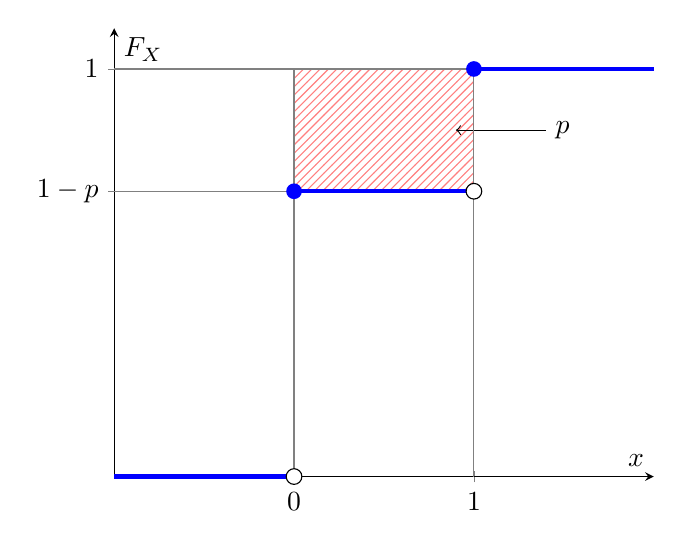
\begin{tikzpicture}
        \begin{axis}[
            clip = false,
            enlargelimits=false,
            axis lines = center,
            %axis equal,
            xlabel = $x$,
            ylabel = $F_X$,
            ymin=0, ymax=1.1,
            xmin=0, xmax=3,
            ytick = {0.7, 1},
            yticklabels={$1-p$, 1},
            xtick={1,2},
            xticklabels={0,1},
        ]        
        \draw[gray] (0,0.7) -- (1,0.7);
        \draw[gray] (0,1) -- (2,1);
        
        \filldraw [draw=gray,pattern=north east lines, pattern color=red!50] (1, 0.7) rectangle (2, 1);
        \draw[<-] (1.9, 0.85) -- (2.4, 0.85) node[anchor=west] {$p$};

        \draw[gray] (1, 0) -- (1, 1);
        \node[blue, circle, fill, inner sep=2pt] at (1, 0.7) {};
        \draw[gray] (2, 0) -- (2, 1);
        \node[blue, circle, fill, inner sep=2pt] at (2, 1) {};
        
        
        
        \draw[blue, ultra thick, inner sep=2pt] (0, 0) -- (1, 0);
        \node[black, circle, draw=black, fill=white, inner sep=2pt] at (1, 0) {};
        
        \draw[blue, ultra thick, inner sep=2pt] (1, 0.7,) -- (2, 0.7);
        \node[black, circle, draw=black, fill=white, inner sep=2pt] at (2, 0.7) {};
        \draw[blue, ultra thick, inner sep=2pt] (2, 1) -- (3, 1);
        \end{axis}
        \end{tikzpicture}
    }
}
    \caption{Rappresentazione grafica di una variabile aleatoria bernoulliana $X \sim B{(p)}$}
    \label{fig:bernoulli}
    \vspace{\abovedisplayskip}
\end{figure}

\noindent Dal grafico della funzione di ripartizione presente in \figurename \ \ref{fig:bernoulli} si evince come $F_X(1)=1$ per qualsiasi variabile aleatoria bernoulliana. Per il \textbf{valore atteso} si può dimostrare inoltre che: \[
\E(X) = \int_0^{1} 1 - F_X(x) dx = P(\text{successo}) = p
\]
\begin{dimostrazione}[$\E(X \sim B{(p)}) = p$]
\begin{align*}
    \E(X) &= {\sum}_x x p_X(x) = \\ 
    &= 0 \cdot p_X(0) + 1 \cdot p_X(1) = \\
    &= p_X(1) = p \tag*{$\blacksquare$}
\end{align*}
\end{dimostrazione}

\noindent Inoltre, per quanto riguarda la \textbf{varianza}: \[
\operatorname{Var}(X) = p(1-p)
\]

\begin{dimostrazione}[$\operatorname{Var}(X \sim B{(p)})$]
\begin{align*}
    \operatorname{Var}(X) &= \E\left((X-\mu)^2\right) =\\
    &= (0-\mu)^2 p_X(0) + (1-\mu)^2 p_X(1) = \\
    &= p^2(1-p) + (1-p)^2p = \\
    &= p(1-p)(\cancel p +1 - \cancel p) = \\
    &= p(1-p)
\end{align*}
alternativamente:
\begin{align*}
    \operatorname{Var}(X) &= \E \left( X^2 \right) - \E(X)^2 = \\
    &= \E(X) - p^2 = \\
    &= p-p^2 = \\
    &= p(1-p) \tag*{$\blacksquare$}
\end{align*}
\end{dimostrazione}

\paragraph{Riproducibilità}
Un processo di Bernoulli è una successione di $n$ variabili aleatorie Bernoulliane \textbf{indipendenti} aventi uguale distribuzione $B{(p)}$. La variabile aleatoria data da questa somma segue una distribuzione \textbf{Binomiale} di parametri $n$ e $p$, vediamola nel dettaglio.

\subsubsection{Modello binomiale $X \sim B{(n,\,p)}$}
Il modello binomiale conta il numero di successi per $n$ esperimenti bernoulliani $p$ \textbf{indipendenti}.\\
Il dominio di $X$ è $D_X = \{ 0, \, \dots, \, n \}$ e i suoi parametri possono assumere valori nei rispettivi intervalli $n \in \{1, \, \dots, \, +\infty\}$ e $0 \leq p \leq 1$.
Trovare $P(X=i)=p_X(i)$ è complicato. Possiamo pensare al modello binomiale come una combinazione di $i$ esperimenti con esito un successo e $n-i$ con esito un fallimento:

\begin{figure}[h]
\vspace{\abovedisplayskip}
\centering
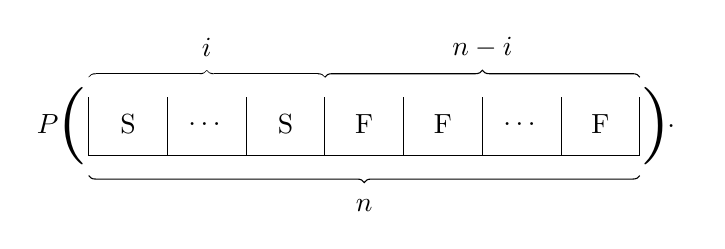
\begin{tikzpicture}
    % scaffale
    \draw[] (0, 0) -- (7, 0);
    \foreach \i in {0, ..., 7} {
        \draw[] (\i, 0) -- (\i, 0.75);
    }
    % s/f
    \node[] at (0.5, 0.4) {S};
    \node[] at (1.5, 0.4) {$\dots$};
    \node[] at (2.5, 0.4) {S};
    \node[] at (3.5, 0.4) {F};
    \node[] at (4.5, 0.4) {F};
    \node[] at (5.5, 0.4) {$\dots$};
    \node[] at (6.5, 0.4) {F};
    
    %\draw[] (5, 0) -- (5, 0.75);
    %\draw[] (6, 0) -- (6, 0.75);
    
    % braces 
    \draw [decorate, decoration={calligraphic brace}] (0, 1) -- (3, 1) node[black, midway, yshift=0.15in] {$i$};
    \draw [decorate, decoration={brace}] (3, 1) -- (7, 1) node[black, midway, yshift=0.15in] {$n-i$};
    \draw [decorate, decoration={brace,mirror}] (0, -0.25) -- (7, -0.25) node[black, midway, yshift=-0.15in] {$n$};
    
    
    % P ( )
    \node[] at (-0.52, 0.4) {$P$};
    \node[scale=2.8] at (-0.2, 0.38) {$($};
    \node[scale=2.8] at (7.2, 0.38) {$)$};
    \node[] at (7.4, 0.38) {$.$};

\end{tikzpicture}
\end{figure}

\begin{figure}[h]
    \centering
\subfloat[Funzione di massa di probabilità]{ 
    \resizebox{7cm}{!}{
        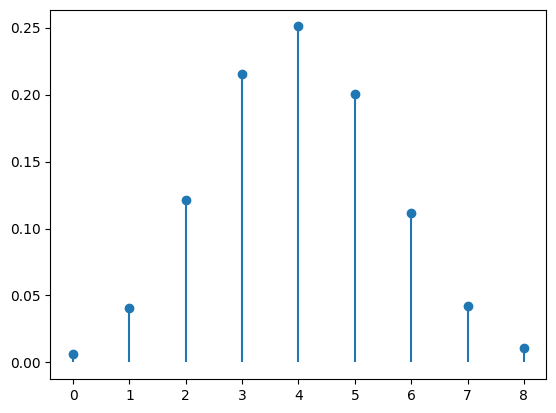
\includegraphics{images/binom_pmf.png}
    }
}
\subfloat[Funzione di ripartizione]{
    \resizebox{7cm}{!}{
        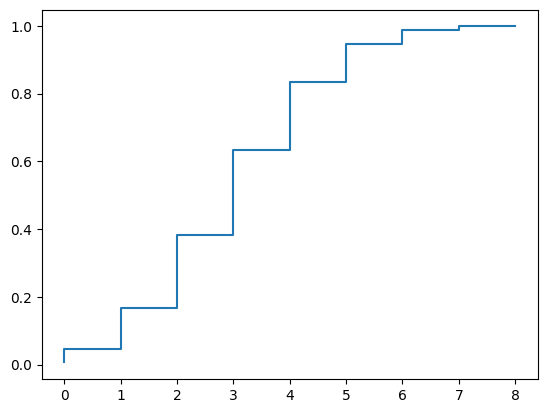
\includegraphics{images/binom_cdf.png}
    }
}
    \caption{Rappresentazione grafica di una variabile aleatoria binomiale $X \sim B{(n, p)}$}
    \label{fig:mod_binom}
    \vspace{\abovedisplayskip}
\end{figure}


\noindent Per controllare se un campione è estratto da una variabile aleatoria che segue un modello binomiale, possiamo controllare la \textbf{forma del grafico} . Una distribuzione binomiale tipica è discreta e ha una forma a campana o a picco, simile a una distribuzione normale, ma discreta. La distribuzione sarà asimmetrica o simmetrica a seconda dei parametri $n$ e $p$. Inoltre, per confutare la nostra tesi possiamo controllare il valore atteso che dovrebbe essere il più alto sulla curva.

\paragraph{Massa di probabilità} Essendo gli esiti indipendenti fra loro, possiamo fattorizzare: \[
P(\text{successo del 1° esp.} \land \text{successo del 2° esp.} \land \dots \land \text{successo dell'$i$-esimo esp.}) = p^i.
\]

\noindent Più in generale, quale è la probabilità di avere le prime $i$ ripetizioni con esito ``successo" e le rimanenti no? \begin{align*}
P(&\text{successo del 1° esp.} \land \dots \land \text{successo dell'i-esimo esp.} \land \phantom{a} \\[-0.3em]
& \! \land \text{fallimento dell'$i+1$-esimo esp.} \land \dots 
\land \text{fallimento dell'$n$ esimo esperimento}) = p^i (1-p)^{n-i}.
\end{align*}

\noindent La probabilità appena calcolata non è $P(X=i)$, perché non è detto che tutti i miei successi siano all'inizio e i fallimenti alla fine, bensì devo moltiplicare per il numero di combinazioni possibili, indicato per ora con $k$: \[
p_X(i) = p^1 (1-p)^{n-1} k
\]

\noindent Il numero di combinazioni semplici è dato da $k = \binom n i$. Inoltre, per annullare il valore di $p_X(i)$ per valori di $i$ fuori dal dominio $D_X$, fattorizziamo la funzione indicatrice $I_{\{ 0, \, \dots, \, n \}}(i)$:

\[
\boxed{p_X(i) = \binom{n}{i} p^i (1-p)^{n-i} I_{\{ 0, \, \dots, \, n \}}(i)}.
\]

\noindent (combinazioni) La somma di tutti gli esiti è naturalmente 1; utilizziamo il binomio di Newton $(a+b)^n = \sum_{i=0}^n \binom n i a^i b^{n-i}$: \[
\sum_{i=0}^n p_X(i) = \sum_{i=0}^n \binom n i p^i (1-p)^{n-i} = (\cancel p+1- \cancel p)^n = 1.
\]

\paragraph{Funzione di ripartizione}
\begin{align*}
F_X(x) &= P(X \leq x) = \\ 
&= P\left( \{ X = 0 \} \cup \{ X = 1 \} \cup \dots \cup \{ X = \lfloor x \rfloor \} \right) = \\
&= \sum_{i=0}^{\lfloor x \rfloor} P(X=i) = \\
&= \sum_{i=0}^{\lfloor x \rfloor} \binom n i p^i (1-p)^{n-i} I_{[0, \, n]}(x) + I_{(n, +\infty)}(x).
\end{align*}

\noindent Da notare come la sommatoria vada da $a$ a $\lfloor x \rfloor$, questo perché $x$ può appartenere ad $\mathbb{R}$.\\
In questo contesto, è necessario moltiplicare per una funzione indicatrice per precludere l'assunzione di valori al di fuori del dominio ($D_X = \{ 0, \, \dots, \, n \}$). Inoltre, si deve aggiungere un'altra funzione indicatrice affinché, se il valore di $x$ supera $n$, il valore assunto dalla funzione di ripartizione sia $1$, come illustrato nella figura \ref{fig:mod_binom} di riferimento.

\paragraph{Valore atteso} Il calcolo del {valore atteso} può essere fatto scomponendo la variabile aleatoria $X$ in $n$ variabili aleatorie $X_i$ che rappresentano l'esito dell'$i$-esimo esperimento bernoulliano $\sim B{(p)}$: $X = \sum_i X_i$. Quindi:
\begin{align*}
\mathbb{E}(X) &= \mathbb{E}\left(\sumi X_i\right) =\\
&= {\sum}_i \mathbb{E}(X_i) = \\ 
&= {\sum}_i p = \\ 
&= n p.
\end{align*}

\paragraph{Varianza} Per la {varianza} possiamo scomporre la sommatoria essendo le $X_i$ indipendenti:
\begin{align*}
\operatorname{Var}(X) &= \operatorname{Var}\left(\sumi X_i\right) = \\ 
&= \sumi \operatorname{Var}(X_i) = \\
&= \sumi p(1-p) = \\
&= n p(1-p).
\end{align*}

\paragraph{Proprietà}
Se consideriamo due variabili aleatorie Binomiali \textbf{aventi lo stesso parametro $p$}, possiamo affermare che la somma di queste due v.a. è ancora una v.a che segue una distribuzione binomiale di parametri $n_1 + n_2$ e $p$. \\

\noindent Sia $X \sim B(n_1, p)$ e $Y \sim B(n_2, p)$, allora:
$$X + Y = K \sim B(n_1, + n_2,  p)$$

\subsubsection{Modello uniforme discreto $X \sim U{(n)}$}
Il modello uniforme discreto è definito in uno spazio di probabilità equiprobabile e l'esperimento casuale che corrisponde a questo modello è l'esperimento che consiste nell'eseguire qualcosa i cui esiti sono $n$ e tutti \textbf{equiprobabili}. Dovendo mappare ogni esito su un numero naturale, conviene considerarli tutti contigui: $D_X = \{1, \, \dots \, , n\}$ con il parametro $n \in \{1, \, \dots, \, +\infty\}$.
\newline \newline
Per determinare se una variabile aleatoria segue una distribuzione uniforme discreta da un grafico, puoi seguire alcune indicazioni e osservare le caratteristiche chiave della distribuzione:
\begin{itemize}
    \item tutte le barre dell'istogramma dovrebbero avere altezze simili o uguali. Questo suggerisce che ogni valore discreto ha la stessa probabilità di occorrenza.
    \item non dovrebbe essere evidente alcun modello specifico nell'istogramma. Non ci dovrebbero essere picchi o valli significativi tra le barre. La distribuzione dovrebbe apparire approssimativamente uniforme, senza evidenziare alcun valore particolare come il più frequente.
    \item la distanza tra le barre dovrebbe essere uniforme e costante. Se i valori discreti sono numeri interi consecutivi, le barre dovrebbero essere equidistanti tra loro.
\end{itemize}

\paragraph{Massa di probabilità} Dalla definizione sappiamo allora che 
\[
\boxed{
p_X(x) = \frac{1}{n} I_{\{1, \, \dots, \, +\infty\}}(x)
}.
\]
\paragraph{Funzione di ripartizione} Anche in questo caso si somma una funzione indicatrice perché se $x > n \, F_X(x) = 1$ 
\begin{align*}
F_X(x) &= P(X \leq x)
= \sum_{i=0}^{\lfloor x \rfloor} p_X(i) = \sum_{i=0}^{\lfloor x \rfloor} \frac{1}{n} = \\ 
&= \frac{\lfloor x \rfloor}{n} I_{[1,n]}(x) + I_{(n, +\infty)}(x).
\end{align*}

\begin{figure}[h]
    \centering
\subfloat[Funzione di massa di probabilità]{
    \resizebox{7cm}{!}{
        \begin{tikzpicture}
        \begin{axis}[
            clip=false,
            enlargelimits=false,
            axis lines = center,
            %axis equal,
            xlabel = $x$,
            ylabel = $p_X$,
            ymin=0, ymax=1.1,
            xmin=0, xmax=4,
            ytick = {1/3, 1},
            yticklabels={$\dfrac 13$, 1},
            xtick={1, 2, 3},
            xticklabels={1, 2, 3},
        ]
        %\addplot[color=blue, thick]{x^2+2};
        \draw[gray] (1, 0) -- (1, 1/3);
        \node[blue, circle, fill, inner sep=2pt] at (1, 1/3) {};
        \draw[gray] (2, 0) -- (2, 1/3);
        \node[blue, circle, fill, inner sep=2pt] at (2, 1/3) {};        
        \draw[gray] (3, 0) -- (3, 1/3);
        \node[blue, circle, fill, inner sep=2pt] at (3, 1/3) {};
        
        \draw[blue, ultra thick, inner sep=2pt] (0, 0) -- (4, 0);
        \node[black, circle, draw=black, fill=white, inner sep=2pt] at (1, 0) {};
        \node[black, circle, draw=black, fill=white, inner sep=2pt] at (2, 0) {};
        \node[black, circle, draw=black, fill=white, inner sep=2pt] at (3, 0) {};
        \end{axis}
        
        \end{tikzpicture}
    }
}
\subfloat[Funzione di ripartizione]{
    \resizebox{7cm}{!}{
        \begin{tikzpicture}
        \begin{axis}[
            clip = false,
            enlargelimits=false,
            axis lines = center,
            %axis equal,
            xlabel = $x$,
            ylabel = $F_X$,
            ymin=0, ymax=1.1,
            xmin=0, xmax=4,
            ytick = {1/3, 2/3, 1},
            yticklabels={$\dfrac 13$, $\dfrac 23$, 1},
            xtick={1,2,3},
        ]
 
        \draw[gray] (1, 0) -- (1, 1/3);
        \node[blue, circle, fill, inner sep=2pt] at (1, 1/3) {};
        \draw[gray] (2, 0) -- (2, 2/3);
        \node[blue, circle, fill, inner sep=2pt] at (2, 2/3) {};
        \draw[gray] (3, 0) -- (3, 1);
        \node[blue, circle, fill, inner sep=2pt] at (3, 1) {}; 
        
        \draw[blue, ultra thick, inner sep=2pt] (0, 0) -- (1, 0);
        \node[black, circle, draw=black, fill=white, inner sep=2pt] at (1, 0) {};
        
        \draw[blue, ultra thick, inner sep=2pt] (1, 1/3) -- (2, 1/3);
        \node[black, circle, draw=black, fill=white, inner sep=2pt] at (2, 1/3) {};
        
        \draw[blue, ultra thick, inner sep=2pt] (2, 2/3) -- (3, 2/3);
        \node[black, circle, draw=black, fill=white, inner sep=2pt] at (3, 2/3) {};
        
        \draw[blue, ultra thick, inner sep=2pt] (3, 1) -- (4, 1);

        \end{axis}
        \end{tikzpicture}
    }
}
    \caption{Rappresentazione grafica di una variabile aleatoria uniforme discreta $X \sim U{(n)}$}
    \label{fig:mod_unif_discr}
\end{figure}

\paragraph{Valore atteso}
\begin{align*}
\mathbb{E}(X) &= \sum_{i=0}^n i \overbrace{p_X(i)}^{\frac{1}{n}} = \sum_{i=0}^n \frac{i}{n} = \\ 
&=\frac{1}{n} \sum_{i=0}^n i = \frac{1}{\cancel{n}} \frac{\cancel{n}(n+1)}{2} = \\ 
&= \frac{n+1}{2}.
\end{align*}

\paragraph{Varianza} La varianza può essere calcolata utilizzando la formula alternativa
$\operatorname{Var}(X) = \mathbb{E}(X^2) - \mathbb{E}(X)^2$:

\begin{align*}
\mathbb{E}(X^2) &= \sum_{i=0}^n i^2 p_X(i) = \sum_{i=0}^n i^2 \frac{1}{n} = \frac{1}{n} \sum_{i=0}^n i^2 = \frac{1}{\cancel{n}} \frac{\cancel{n}(n+1)(2n+1)}{6} = \frac{2n^2 + 3n + 1}{6} \\
%
\mathbb{E}(X)^2 &= \left (\frac{n+1}{2} \right )^2 = \frac{n^2 + 2n + 1}{4} \\
%
\operatorname{Var}(X) &= \mathbb{E}(X^2) - \mathbb{E}(X)^2 = \frac{2n^2 + 3n + 1}{6} - \frac{n^2 + 2n + 1}{4} = \frac{4n^2 + 6n + 2 - 3n^2 - 6n - 3}{12} = \frac{n^2 - 1}{12}
\end{align*}



\subsubsection{Modello uniforme continuo $X \sim U{(a,\,b)}$}
Il modello uniforme continuo è definito da due parametri $a,b$ con $a < b$ e $a ,\, b \in \mathbb R$ indicanti gli estremi dell'intervallo di definizione: infatti, come nel modello uniforme discreto dove $n$ indicava il numero di specificazioni con supporto $D_X = \{1, \, \dots ,\, n\}$, nel continuo è $D_X = [a,\,b]$ (è importante notare come non ci sia differenza se l'intervallo è aperto o chiuso, questo perché l'integrale in un punto vale $0$). 
\newline \newline
Per determinare se una variabile aleatoria segue una distribuzione uniforme continua da un grafico, puoi seguire alcune indicazioni e osservare le caratteristiche chiave della distribuzione:
\begin{itemize}
    \item la densità di probabilità è costante su tutto l'intervallo specificato. Ciò significa che la probabilità di ottenere un valore in qualsiasi sottointervallo dell'intervallo definito è la stessa.
    \item l'altezza della curva dovrebbe essere costante su tutto l'intervallo. Questo indica che ogni punto all'interno dell'intervallo ha la stessa probabilità di essere osservato.
    \item l'intervallo su cui è definita la distribuzione uniforme continua dovrebbe essere chiaramente indicato nel grafico. La PDF ha valore zero al di fuori di questo intervallo.
    \item la distribuzione dovrebbe apparire approssimativamente uniforme su tutto l'intervallo, senza evidenziare alcun punto particolare come il più probabile.
\end{itemize}

\paragraph{Densità di probabilità} La funzione di densità di probabilità $f_X(x)$ deve essere costante ($f_X(x) = \alpha$) nel caso in cui $x$ assume un valore del dominio, 0 altrimenti. 

%Dobbiamo trovare anche qua una funzione di "massa" di probabilità $f_X(x)$ che sia costante nei casi in cui $x$ assume un valore del dominio e sia $0$ altrimenti \\
\noindent Scriviamo $f_X(x)$ come $\alpha I_{[a,\,b]}(x)$ e troviamo $\alpha$ applicando la relazione $\int_{-\infty}^{+\infty} f_X(x) dx = 1$:
\begin{align*}
\int_{-\infty}^{+\infty} f_X(x) dx &= \int_a^b f_X(x) dx = \int_a^b \alpha dx = \alpha \int_a^b dx = \\
&= \alpha [x]^b_a = \alpha (b-a) = 1\\
&\Rightarrow {\alpha = \frac{1}{b-a}};
\end{align*}
scriviamo allora:
$$
\boxed{f_X(x) = \frac{1}{b-a} I_{[a,\,b]}(x)}
$$

\paragraph{Funzione di ripartizione}
Calcolando $F_X(x) = P(X \leq x) = \int_{-\infty}^x f_X(y) dy$, ci accorgiamo che questo integrale ha senso solo se $x \in D_X$. Supponendo quindi $x \in D_X$, possiamo modificare l'intervallo dell'integrale in $[a, \, x]$:
\begin{align*}
    F_X(x) &= \int_a^x f_X(y) dy = \int_a^x \frac{1}{b-a} dy = \\
    &= \frac{1}{b-a} \int_a^x dy = \frac{1}{b-a} [y]^x_a = \\ 
    &= \frac{x-a}{b-a} I_{[a,\,b]}(x) + I_{(b, \,+\infty)}(x).
\end{align*}
Dal punto di vista geometrico, questo grafico è una retta che passa per i punti $(a,\,0)$ e $(b,\,1)$. \\

\begin{figure}[h]
    \centering
\subfloat[Funzione di densità di probabilità]{
    \resizebox{7cm}{!}{
        \begin{tikzpicture}
        \begin{axis}[
            clip=false,
            enlargelimits=false,
            axis lines = center,
            %axis equal,
            xlabel = $x$,
            ylabel = $p_X$,
            ymin=0, ymax=1.1,
            xmin=0, xmax=4,
            ytick = {1/3, 1},
            yticklabels={$\dfrac 1{b-a}$, 1},
            xtick={1, 3},
            xticklabels={$a$, $b$},
        ]
        %\addplot[color=blue, thick]{x^2+2};
        \draw[gray] (1, 0) -- (1, 1/3);
        \node[blue, circle, fill, inner sep=2pt] at (1, 1/3) {};
        %\draw[gray] (2, 0) -- (2, 1/3);
        %\node[blue, circle, fill, inner sep=2pt] at (2, 1/3) {};        
        \draw[gray] (3, 0) -- (3, 1/3);
        \node[blue, circle, fill, inner sep=2pt] at (3, 1/3) {};
        
        \draw[blue, ultra thick, inner sep=2pt] (0, 0) -- (1, 0);
        \draw[blue, ultra thick, inner sep=2pt] (1, 1/3) -- (3, 1/3);
        \draw[blue, ultra thick, inner sep=2pt] (3, 0) -- (4, 0);
        \node[black, circle, draw=black, fill=white, inner sep=2pt] at (1, 0) {};
        %\node[black, circle, draw=black, fill=white, inner sep=2pt] at (2, 0) {};
        \node[black, circle, draw=black, fill=white, inner sep=2pt] at (3, 0) {};
        \end{axis}
        
        \end{tikzpicture}
    }
}
\subfloat[Funzione di ripartizione]{
    \resizebox{7cm}{!}{
        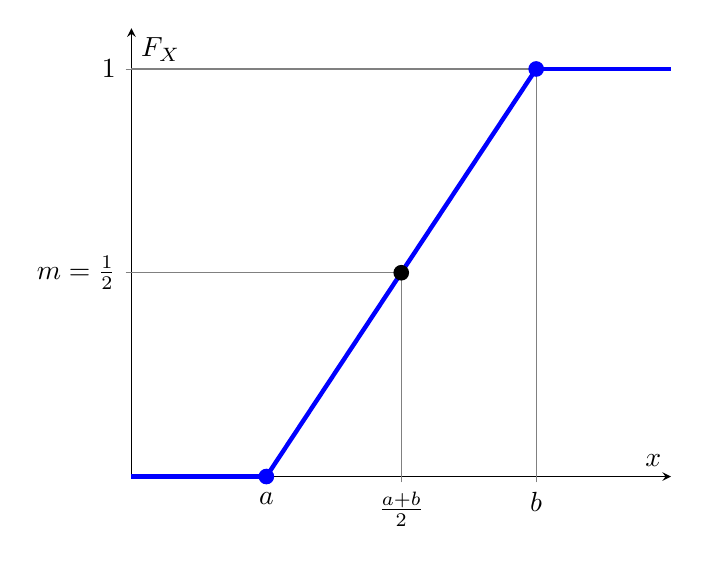
\begin{tikzpicture}
        \begin{axis}[
            clip = false,
            enlargelimits=false,
            axis lines = center,
            %axis equal,
            xlabel = $x$,
            ylabel = $F_X$,
            ymin=0, ymax=1.1,
            xmin=0, xmax=4,
            ytick = {1/2, 1},
            yticklabels={$m = \frac{1}{2}$, 1},
            xtick={1,2,3},
            xticklabels={$a$, $\frac {a+b}{2}$, $b$},
        ]
    %\filldraw [draw=gray,pattern=north west lines, pattern color=red!50] (0, 0) rectangle (1, 1);
    %\filldraw [draw=gray,pattern=north east lines, pattern color=red!50] (0, 1/2) rectangle (2, 5/6);
    %\node[isosceles triangle, isosceles triangle stretches,
    minimum height = 2cm, 
    minimum width= 1cm, 
    shape border rotate=-50,
    fill=cyan!30, ] (T30)at (2,1/2){};
        
    \draw[gray] (2, 0) -- (2, 1/2);
    \draw[gray, name path=L] (0, 1/2) -- (2, 1/2);
    \draw[gray] (0, 1) -- (3, 1);
    %\draw[gray] (1, 0) -- (1, 1);
    
    \draw[gray] (3, 0) -- (3, 1);
    \node[blue, circle, fill, inner sep=2pt] at (3, 1) {}; 
    
    \draw[blue, ultra thick, inner sep=2pt] (1, 0) -- (3, 1);
    
    \draw[blue, ultra thick, inner sep=2pt] (0, 0) -- (1, 0);
    \node[blue, circle, fill, inner sep=2pt] at (1, 0) {};

    \draw[blue, ultra thick, inner sep=2pt] (3, 1) -- (4, 1);
    
    \node[black, circle, fill, inner sep=2pt] at (2, 1/2) {};
    
    \end{axis}
    \end{tikzpicture}
    }
}
    \caption{Rappresentazione grafica di una variabile aleatoria uniforme continua $X \sim U{(a, \, b)}$}
    \label{fig:mod_unif_cont}
\end{figure}

\paragraph{Valore atteso}
Per calcolare il {valore atteso} possiamo applicare la formula $\int_0^{+\infty} 1 - F_X(x) dx$, ma questo vale solo nel caso in cui $X \geq 0$.
Applichiamo allora la definizione di valore atteso, ovvero
\begin{align*}
\mathbb{E}(X) &= \int_{-\infty}^{+\infty} x f_X(x) dx = \int_a^b \frac{x}{b-a} dx = \\ 
&= \frac{1}{b-a} \left [\frac{x^2}{2} \right ]_a^b = \frac{b^2 - a^2}{2 (b-a)} = \\
&= \frac{\cancel{(b-a)}(b+a)}{2 \cancel{(b-a)}} = \frac{a+b}{2}.
\end{align*}

\paragraph{Varianza}
Manca infine la {varianza}, che andiamo a calcolare usando la formula alternativa
\begin{align*}
\mathbb{E}(X)^2 &= \left (\frac{a+b}{2} \right) ^ {\!\!2} = \frac{a^2 + b^2 + 2ab}{4} \\
%
\mathbb{E}(X^2) &= \int_{-\infty}^{+\infty} x^2 f_X(x) dx = \int_a^b \frac{x^2}{b-a} dx = \frac{1}{b-a} \left [\frac{x^3}{3} \right ]_a^b = \frac{b^3 - a^3}{3 (b-a)} = \frac{\cancel{(b-a)}(a^2 + b^2 + ab)}{3 \cancel{(b-a)}} = \frac{a^2 + b^2 + ab}{3} \\
%
\operatorname{Var}(X) &= \mathbb{E}(X^2) - \mathbb{E}(X)^2 = \frac{a^2 + b^2 + ab}{3} - \frac{a^2 + b^2 + 2ab}{4} = \frac{4a^2 + 4b^2 + 4ab - 3a^2 - 3b^2 - 6ab}{12} = \frac{(b-a)^2}{12}
\end{align*}

\noindent Notiamo che, come nel modello uniforme discreto, la varianza ha ancora 12 come denominatore, inoltre questo risultato dipende dal quadrato della distanza tra $a$ e $b$. \\

\noindent Ricordando inoltre che esiste la proprietà tale per cui $P(m \leq X \leq l) = F(l) - F(m)$, e tenendo a mente che gli estremi non sono necessariamente inclusi perché siamo nell'ambito delle v.a. continue, possiamo dire che nel modello uniforme continuo $$P(m \leq X \leq l) = F(l) - F(m) = \frac{l - a}{b - a} - \frac{m - a}{b - a} = \frac{l - m}{b - a}$$

\subsubsection{Modello geometrico $X \sim G{(p)}$}
Il modello geometrico consiste nell'esecuzione ripetuta, potenzialmente in modo infinito, di esperimenti bernoulliani di parametro $p$ in condizioni di \textbf{indipendenza} e \textbf{identicamente distribuiti}; la sequenza termina quando l'$i$-esimo esito è un successo.
In poche parole, il modello geometrico conta il \textbf{numero di fallimenti} fino a quando non si ottiene un successo. \\
A differenza del modello binomiale dove è fissato un numero massimo di esperimenti consecutivi, nel modello geometrico la sequenza è \textbf{potenzialmente infinita}. 
Facendo un parallelo con i linguaggi di programmazione, il modello binomiale è un $\textit{for}$ mentre il modello geometrico è un ciclo $\textit{while}$. \\ \\
Notiamo subito che $0 < p \leq 1$: infatti, se $p = 0$ allora il ``ciclo" non terminerebbe mai, facendo assumere a $X$ il valore $+\infty$ (assurdo per una variabile aleatoria). Altro caso degenere è $p=1$: in questo caso $X = 0$. Il supporto di $X$ è $D_X = \{0, \, \dots ,\, +\infty\} = \mathbb{N} \cup 0$.
\newline \newline
Per capire se un set di dati segue una distribuzione geometrica da un grafico, puoi eseguire le seguenti analisi:
\begin{itemize}
    \item \textbf{Forma della distribuzione}: La distribuzione geometrica ha una caratteristica forma a coda lunga verso destra. Questo significa che ci sono poche occorrenze di valori elevati e molte occorrenze di valori bassi. La probabilità di ottenere il primo successo al tentativo $k$ è data dalla formula $P(X = k) = (1 - p)^{k-1} p$, dove $p$ è la probabilità di successo in ogni tentativo. La probabilità diminuisce con l'aumentare del numero di tentativi.
    \item \textbf{Probabilità di successo}: Verifica se la probabilità di successo $p$ è costante e che ogni valore rappresenti il numero di tentativi necessari per ottenere il primo successo. Nei dati, la probabilità di ottenere il primo successo dovrebbe diminuire esponenzialmente con l'aumentare del numero di tentativi, come previsto dalla formula della distribuzione geometrica.
    \item \textbf{Moda della distribuzione}: La moda della distribuzione geometrica è $k = 1$, il che significa che il primo tentativo è il più probabile per ottenere il successo. Dai un'occhiata al grafico per vedere se il valore $1$ è quello più frequente tra i dati. Questo è un indicatore che i dati potrebbero seguire una distribuzione geometrica.

\end{itemize}

\paragraph{Massa di probabilità}
\begin{figure}[h]
    \centering
\subfloat[Funzione di massa di probabilità]{
    \resizebox{7cm}{!}{
        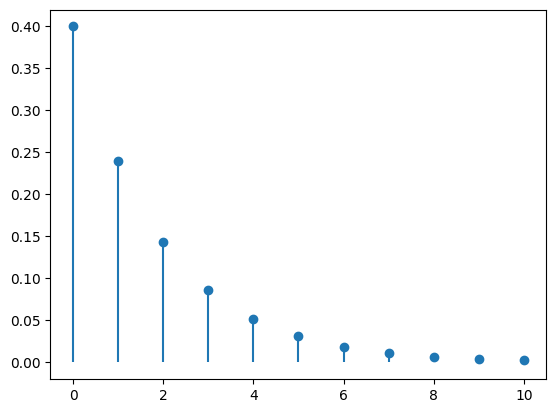
\includegraphics{images/geom_pmf.png}
    }
}
\subfloat[Funzione di ripartizione]{
    \resizebox{7cm}{!}{
        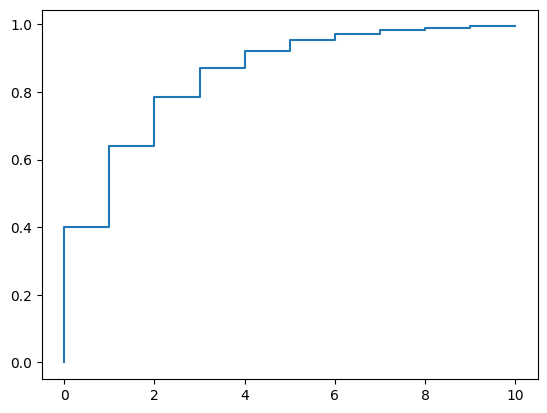
\includegraphics{images/geom_cdf.png}
    }
}
    \caption{Rappresentazione grafica di una variabile aleatoria geometrica $X \sim g{(p)}$}
    \label{fig:mod_geom}
    \vspace{\abovedisplayskip}
\end{figure}

Calcoliamo $p_X(i) = P(X = i)$: questo significa calcolare la probabilità che i primi $i$ esperimenti siano insuccessi (indicati con F) e che l'$(i+1)$-esimo esperimento sia un successo.

\hspace{14pt}
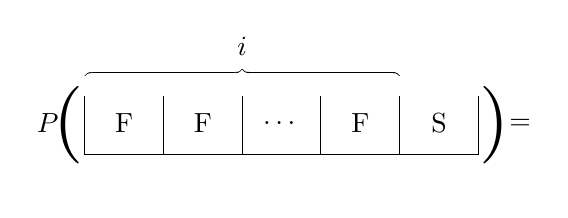
\begin{tikzpicture}
    % scaffale
    \draw[] (0, 0) -- (5, 0);
    \foreach \i in {0, ..., 5} {
        \draw[] (\i, 0) -- (\i, 0.75);
    }
    % s/f
    \node[] at (0.5, 0.4) {F};
    \node[] at (1.5, 0.4) {F};
    \node[] at (2.5, 0.4) {\dots};
    \node[] at (3.5, 0.4) {F};
    \node[] at (4.5, 0.4) {S};
    
    % braces 
    \draw [decorate, decoration={calligraphic brace}] (0, 1) -- (4, 1) node[black, midway, yshift=0.15in] {$i$};
    
    % P ( )
    %\node[] at (-0.52, 0.4) {$P$};
    \node[] at (-0.47, 0.4) {$P$};
    \node[scale=2.8] at (-0.2, 0.38) {$($};
    \node[scale=2.8] at (5.2, 0.38) {$)$};
    \node[] at (5.53, 0.38) {$=$};
\end{tikzpicture}
% riduzione spazio tra immagine e align
\vspace{-10pt}
%
\begin{align*}
&= P(\textnormal{1° esito insuccesso} \cap \textnormal{2° esito insuccesso} \cap \dots \cap \textnormal{$i$° esito insuccesso} \cap \textnormal{$(i+1)$° esito successo}) = \\ 
&= \prod_{j=1}^i P(j) \cdot P(\{(i+1) \text{° successo}\})  = \prod_{j=1}^i (1-p) \cdot p = p(1-p)^i I_{\{0, \, \dots, \, +\infty\}}(i).
\end{align*}
Il grafico denota un \textbf{decadimento esponenziale} che è più o meno accentuato in base a quanto $p$ è vicino a 1. \\ \\
Controlliamo se la somma di tutti i possibili valori di $p_X(i)$ è uguale a $1$:
\begin{align*}
\sum_{i=0}^{+\infty} p_X(i) &= \sum_{i=0}^{+\infty} p(1-p)^i = p \sum_{i=0}^{+\infty} (1-p)^i;
\intertext{
ma questa è una \textit{serie geometrica} di ragione $q = 1 - p$; notiamo che $|q| < 1$ (quindi quando $q$ è compreso tra $1$ e $-1$) quindi la sua somma converge a $\frac{1}{1 - q}$}
&= p \sum_{i=0}^{+\infty} (1-p)^i = \cancel{p} \cdot \frac{1}{{\cancel{1 - (1-p)}}} = 1.
\end{align*}
\begin{proprieta}
\label{prop:one}
\noindent La seguente relazione sarà utile per il calcolo del valore atteso e della varianza.
\begin{align*}
    \sum_{i=0}^{+\infty} i \alpha^i &= \alpha \sum_{i=0}^{+\infty} i \alpha^{i-1} = \alpha \sum_{i=0}^{+\infty} \frac{d}{d\alpha} \alpha^i = \alpha \frac{d}{d\alpha} \left [ \sum_{i=0}^{+\infty} \alpha^i \right ] =
\intertext{considerando $|\alpha| < 1$, ovvero $-1 < \alpha < 1$ allora}
&= \alpha \frac{d}{d\alpha} \left [ \sum_{i=0}^{+\infty} \alpha^i \right ] = \alpha \frac{d}{d\alpha} \left(\frac{1}{1 - \alpha}\right) = \frac{\alpha}{(1 - \alpha)^2}
\end{align*}
\end{proprieta}
\noindent Sapendo che la serie $\sum_{i=0}^{+\infty} a^i$ converge uniformemente per valori di $\alpha$ compresi tra $-1 \textnormal{ e } 1$ possiamo sfruttare la proprietà tale per cui è possibile scambiare derivata e sommatoria.
\paragraph{Valore atteso} Calcoliamo il valore atteso come
\begin{align*}
\mathbb{E}(X) &= \sum_{i=0}^{+\infty} i p_X(i) = \sum_{i=0}^{+\infty} i p(1-p)^i = p \sum_{i=0}^{+\infty} i (1-p)^i;
\intertext{in questo caso $\alpha = 1 -p$, quindi}
&= p \sum_{i=0}^{+\infty} i (1-p)^i = \cancel{p} \frac{1-p}{p^{\cancel 2}} = \frac{1-p}{p}.
\end{align*}

\paragraph{Varianza} Calcoliamo infine la varianza usando la formula alternativa; calcoliamo quindi $\E(X^2)$
\begin{align*}
\mathbb{E}\left(X^2\right) &= \sum_{i=0}^{+\infty} i^2 p_X(i) \\
&= \sum_{i=0}^{+\infty} i^2 p(1-p)^i \\
&= p(1-p) \sum_{i=0}^{+\infty} i^2 (1-p)^{i-1}
\intertext{notiamo come $i^2(1-p)^{i-1}$ è la derivata di $-i(1-p)^i$, quindi possiamo applicare la Proprietà \ref{prop:one}}
&= p(1-p) \sum_{i=0}^{+\infty} \frac{d}{dp} \left(-i(1-p)^i\right) \\
&= - p(1-p) \frac{d}{dp} \left (\sum_{i=0}^{+\infty} i(1-p)^i \right ) \\ 
&= - p(1-p) \frac{d}{dp} \left ( \frac{1-p}{p^2} \right )
\intertext{deriviamo e ricaviamo il valore finale}
&= - p(1-p) \frac{-p^2 - (1-p)2p}{p^4} \\ 
&= -(1-p) \frac{-p^2 -2p +2p^2}{p^3} \\ 
&= -\frac{p(1-p)(p-2)}{p^3} \\ 
&= \frac{(1-p)(2-p)}{p^2}.
\intertext{Ora possiamo finalmente calcolare la varianza}
\operatorname{Var}(X) &= \mathbb{E}\left(X^2\right) - \mathbb{E}(X)^2 \\ 
&= \frac{(1-p)(2-p)}{p^2} - \left (\frac{1-p}{p} \right )^2 \\ 
&= \frac{p^2 - 3p + 2 - p^2 + 2p - 1}{p^2} = \frac{1 - p}{p^2}
\end{align*}

\paragraph{Funzione di ripartizione} 
Per calcolare la funzione di ripartizione è necessario aggiungere una proprietà:

\begin{proprieta}
\label{prop:two}
Sia $n \in \mathbb{N}$, calcoliamo
\begin{align*}
P(X > n) &= P(X \geq n+1) \\
&= P(X = n+1 \, \vee X = n+2 \, \vee \dots) \\ 
&= \sum_{i = n+1}^{+\infty} P(X = i)
\intertext{la somma infinita di probabilità disgiunte è possibile solo nel caso di $\sigma$-algebre; 
Malchiodi ci ha indicato di assumere che in questo caso si possa fare. Estraiamo inoltre $(1-p)^{n+1}$ dalla sommatoria}
&= \sum_{i = n+1}^{+\infty} p(1-p)^i \\ 
&= p(1-p)^{n+1} \sum_{i = n+1}^{+\infty} (1-p)^i (1-p)^{-n-1}
\intertext{arrangiamo la sommatoria introducendo $j = i - (n+1)$ per ottenere una serie geometrica}
&= p(1-p)^{n+1} \sum_{j = 0}^{+\infty} (1-p)^j \\ 
&= p(1-p)^{n+1} \frac{1}{1 - (1-p)} = (1-p)^{n+1}.
\end{align*}
\end{proprieta}
\noindent Utilizzando quindi la Proprietà \ref{prop:two} possiamo dimostrare che
\begin{align*}
F_X(x) &= P(X \leq x) = 1 - P(X > x) = \\
&= 1 - P(X \geq x + 1) = \\ 
&= 1 - (1-p)^{x+1}.
\intertext{Essendo il dominio della variabile aleatoria solo numeri interi, possiamo aggiungere una funzione indicatrice e riscrivere la funzione di ripartizione come}
&= (1 - (1 - p)^{\lfloor x \rfloor + 1}) I_{[0, +\infty)}(x).
\end{align*}
\paragraph{Assenza di memoria} L'assenza di memoria è un'interessante proprietà posseduta da solo due modelli. \\
Sia $X = t$ una variabile aleatoria che indica che al tempo $t$ è successo un certo evento; vogliamo calcolare $P(X \geq i + j \ | \ X \geq i)$, ovvero la probabilità condizionata di terminare la sequenza dopo $i+j$ iterazioni sapendo che ne sono già state eseguite almeno $i$:
\begin{align*}
P(X \geq i) &= P(X > i - 1) = (1-p)^i \\
\boxed{P(X \geq i + j \ | \ X \geq i)} &= \frac{P(X \geq i + j \ \cap \ X \geq i)}{P(X \geq i)} = \frac{P(X \geq i + j)}{(1-p)^i} = \\
&= \frac{(1-p)^{i+j}}{(1-p)^i} = (1-p)^j = \boxed{P(X \geq j)}
\end{align*}

\noindent Abbiamo ottenuto che $P(X \geq i + j \ | \ X \geq i) = P(X \geq j)$: questo risultato è molto interessante perchè anche dopo $i$ iterazioni la probabilità che le prossime $j$ siano un insuccesso non cambia.

\subsubsection{Modello di Poisson $X \sim P{(\lambda)}$}
\begin{figure}[h]
    \centering
\subfloat[Funzione di massa di probabilità]{
    \resizebox{7cm}{!}{
        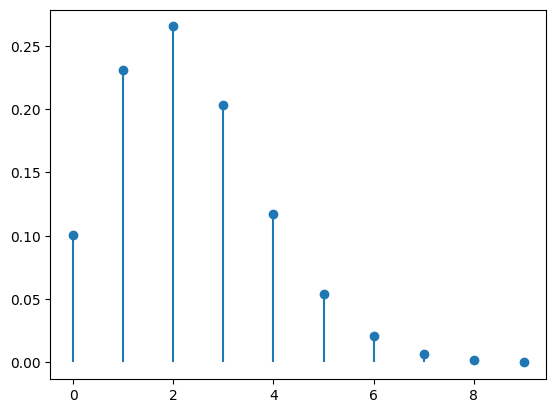
\includegraphics{images/poisson_pmf.png}
    }
}
\subfloat[Funzione di ripartizione]{
    \resizebox{7cm}{!}{
        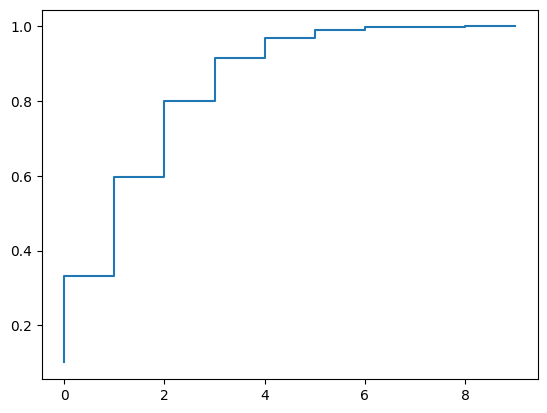
\includegraphics{images/poisson_cdf.png}
    }
}
    \caption{Rappresentazione grafica di una variabile aleatoria di Poisson $X \sim P{(\lambda)}$}
    \label{fig:mod_poisson}
    %\vspace{\abovedisplayskip}
\end{figure}
\noindent Il modello di Poisson è un tipo di distribuzione di probabilità discreta utilizzata per modellare il numero di eventi rari che si verificano in un intervallo fisso di tempo o spazio, dato che gli eventi si verificano in modo casuale e indipendente con una bassa probabilità di successo per ogni intervallo di tempo o spazio. Il parametro chiave della distribuzione di Poisson è $\lambda$, che rappresenta il tasso di eventi medi che si verificano in un dato intervallo di tempo o spazio. Inoltre assume che gli eventi siano indipendenti l'uno dall'altro, ciò significa che la probabilità di un evento non influenza la probabilità degli altri eventi.
\newline
Alcune applicazioni comuni includono il conteggio di chiamate telefoniche in un call center, il conteggio di incidenti stradali in un determinato periodo di tempo, il conteggio di particelle radioattive in un campione, e molte altre.
\newline \newline
Per determinare se un set di dati segue il modello di Poisson, è possibile utilizzare un approccio visivo e statistiche descrittive:
\begin{itemize}
    \item la distribuzione di Poisson ha una forma asimmetrica con una coda lunga verso destra. Verifica se i dati mostrano questa caratteristica forma asimmetrica.
    \item verifica se la forma del grafico dei dati è coerente con il valore di $lambda$. Ad esempio, se $lambda$ è relativamente grande, ti aspetteresti di vedere una maggiore concentrazione di dati intorno al parametro.
    \item se i dati seguono il modello di Poisson, dovresti trovare che la media campionaria è simile o vicina al parametro $lambda$, e la varianza campionaria dovrebbe essere approssimativamente uguale a $lambda$.
\end{itemize}

\paragraph{Massa di probabilità}
Una variabile aleatoria $X$ si dice seguire il modello di Poisson, avente supporto $D_X = \{0, \, ..., \, +\infty\}$, se dato un $\lambda \in (0, +\infty)$:
\[
\boxed{
p_X(i) = e^{-\lambda} \frac{\lambda^i}{i!} I_{\{0, \, \dots, \, +\infty\}}(i)
}.
\]
Verifichiamo che la somma di tutte le probabilità sia 1: \begin{align*}
    \sum_{i=0}^{+\infty} p_X(i) &= \sum_{i=0}^{+\infty} e^{-\lambda} \frac{\lambda^i}{i!} = \\
    &= e^{-\lambda} \sum_{i=0}^{+\infty} \frac{\lambda^i}{i!} = 
    \intertext{la sommatoria rappresenta lo sviluppo in serie di Taylor di $\displaystyle e^\lambda$, quindi:}
    &= e^{-\lambda}e^{\lambda} = 1.
\end{align*}


\paragraph{Valore atteso}
\begin{align*}
    \E(X) &= \sum_{i=0}^{+\infty} i p_X(i) = \\
    &= \sum_{i=1}^{+\infty} i e^{-\lambda} \frac{\lambda^i}{i!} = \\
    &= e^{-\lambda} \sum_{i=1}^{+\infty} i \frac{\lambda^i}{i!} = 
    \intertext{tentiamo di avere $i-1$ nella sommatoria:}
    &= e^{-\lambda} \sum_{i=1}^{+\infty} \frac{\lambda^i}{(i-1)!} = \\
    &= \lambda e^{-\lambda} \sum_{i=1}^{+\infty} \frac{\lambda^{i-1}}{(i-1)!} = \\
    \intertext{poniamo quindi $j = i-1$ e riapplichiamo lo sviluppo in serie di Taylor:}
    &= \lambda e^{-\lambda} \sum_{j=0}^{+\infty} \frac{\lambda^j}{j!} = \\
    &= \lambda e^{-\lambda} e^{\lambda} = \lambda.
\end{align*}
\noindent Si noti come inizialmente l'indice della sommatoria $i$ parta da $0$, e successivamente viene posto a $1$. Questo perché quando $i$ vale $0$ si annulla tutto, essendoci una moltiplicazione per $i$, quindi quella somma non influirà sul risultato finale.
\paragraph{Varianza} Anche qui usiamo il metodo alternativo per il calcolo della varianza.
\begin{align*}
    \E(X^2) &= \sum_{i=0}^{+\infty} i^2 e^{-\lambda} \frac{\lambda^i}{i!} = 
    \intertext{come per il valore atteso, tentiamo di avere $i-1$ nella sommatoria:}
    &= e^{-\lambda} \sum_{i=1}^{+\infty} i \frac{\lambda^i}{(i-1)!} =
    \intertext{per trasformare la $i$ nella sommatoria in $i-1$, scriviamo $((i-1)+1)$:}
    &= \lambda e^{-\lambda} \sum_{i=1}^{+\infty} ((i-1)+1) \frac{\lambda^{i-1}}{(i-1)!} = \\
    &= \lambda e^{-\lambda} \sum_{i=1}^{+\infty} (i-1) \frac{\lambda^{i-1}}{(i-1)!} + \lambda e^{-\lambda} \sum_{i=1}^{+\infty} \frac{\lambda^{i-1}}{(i-1)!} =
    \intertext{poniamo quindi $j = i-1$ e riapplichiamo lo sviluppo in serie di Taylor:}
    &= \lambda e^{-\lambda} \sum_{j=0}^{+\infty} j \frac{\lambda^j}{j!} + \lambda e^{-\lambda} \sum_{j=0}^{\lambda} \frac{\lambda^j}{j!} = \\
    &= \lambda e^{-\lambda} \sum_{j=1}^{+\infty} \cancel{j} \frac{\lambda^{j}}{\cancel{j}(j-1)!} + \lambda \cancel{e^{-\lambda}} \cancel{e^{\lambda}} = \\
    &= \lambda e^{-\lambda} \sum_{j=1}^{+\infty} \lambda \frac{\lambda^{j-1}}{(j-1)!} + \lambda = \\
    \intertext{poniamo quindi $k = j-1$ e riapplichiamo lo sviluppo in serie di Taylor ancora una volta:}
    &= \lambda e^{-\lambda} \lambda \sum_{k=1}^{+\infty} \frac{\lambda^{k}}{(k)!} + \lambda = \\
    &= \lambda^2 + \lambda.
\end{align*}
Quindi:
\begin{align*}
    \operatorname{Var}(X) &= \E(X^2) - \E(X)^2 \\
    &= (\lambda^2 + \lambda) - (\lambda)^2 = \lambda.
\end{align*}

\paragraph{Relazione tra il m.\ di Poisson e il m.\ binomiale}
Data $X \sim B{(n, \, p)}$ una variabile aleatoria binomiale, possiamo ricavare una relazione che lega $X$ ad una variabile aleatoria di Poisson per $n$ molto grande ($n \to +\infty$) e $p$ molto piccolo. \\ Partendo dal modello binomiale e fissando $n p = \lambda$, scriviamo la funzione di massa di probabilità:
\begin{align*}
    P(X=i) &= \binom{n}{i} p^i(1-p)^{n-i} = \\
    &= \frac{n!}{i!(n-i)!} p^i (1-p)^{n-i} = 
    \intertext{sappiamo che $\displaystyle p = \frac{np}{n} = \frac{\lambda}{n}$, quindi:}
    &= \frac{n(n-1)\dots (n-i+1) \cancel{(n-i)!}}{i! \cancel{(n-i)!}} \left(\frac{\lambda}{n}\right)^i \left(1-\frac{\lambda}{n}\right)^{\!\!n-i} = \\
    &= \frac{n(n-1)\dots (n-i+1)}{n^i} \ \frac{\lambda^i}{i!} \left(1 - \frac{\lambda}{n}\right)^{n-i} = \\
    &= \frac{n(n-1)\dots (n-i+1)}{n\cdot \, \dots \, \cdot n} \ \frac{\lambda^i}{i!} \left(1 - \frac{\lambda}{n}\right)^{n-i} =
    \intertext{nella prima frazione ci sono $i$ termini sia al numeratore che al denominatore che tendono a $1$ se $n \to +\infty$:}
    &= \cancelto{1}{\frac{n(n-1)\dots (n-i+1)}{n\cdot \, \dots \, \cdot n}} \ \frac{\lambda^i}{i!} \frac{\left(1 - \frac{\lambda}{n}\right)^{n}}{\left(1 - \frac{\lambda}{n}\right)^{i}} =
    \intertext{se $n \to +\infty$ allora il denominatore della seconda frazione tende a $1$ mentre il numeratore tende a $e^{-\lambda}$, considerando il limite notevole dato del numero di nepero  $\lim_{x \to \infty} \left ( 1 + \frac{a}{x} \right )^x = e^{\alpha}$ sostituendo $\alpha$ con $-\lambda$:}
    &= \frac{\lambda^i}{i!} e^{-\lambda}
\end{align*}
Questa relazione è estremamente utile perché il risultato non è dipendente da $n$. Possiamo descrivere ciò che abbiamo appena mostrato come una v.a. con distribuzione approssimativamente di Poisson con valore atteso $n p = \lambda$  in cui il totale dei successi in un gran numero di ripetizioni \textbf{indipendenti} ($n$) di un esperimento il quale ha una piccola probabilità di riuscita ($p$).


\paragraph{Riproducibilità}
{Il modello di Poisson gode}
della proprietà di riproducibilità, ovvero date due variabili aleatorie $X_1$ e $X_2$ indipendenti che seguono la distribuzione di Poisson di parametro $\lambda_1$ e $\lambda_2$ rispettivamente, allora:
\[
X_1 \sim P{(\lambda_1)} \land X_2 \sim P{(\lambda_2)} \Rightarrow X_1 + X_2 \sim P{(\lambda_1 + \lambda_2)}
\]
se le due variabili aleatorie sono anche identicamente distribuite, allora possiamo scrivere
\[
X_1 + X_2 \sim P{(2\lambda)}
\]

\subsubsection{Modello ipergeometrico $X \sim \mathcal H{(n, \, M, \, N)}$}
Possiamo pensare al modello binomiale come all'estrazione da un'urna che contiene $2$ tipi di oggetti; l'estrazione avviene con re-immissione perché ad ogni estrazione (esperimento bernoulliano) si ha sempre la stessa probabilità di estrarre un oggetto del primo tipo (o del secondo tipo); nel modello ipergeometrico invece si effettuano delle estrazioni senza la re-immissione. \\
Indichiamo con: \begin{itemize}
    \item $N$ il numero di oggetti ``funzionanti" $N \in \{0, \,1, \, ... , \, n\}$,
    \item $M$ il numero di oggetti ``difettosi" $M \in \{0, \,1, \, ... , \, n\}$,
    \item $n$ il numero di estrazioni $n \in \mathbb N^+$,
\end{itemize}
allora la variabile aleatoria $X \sim \mathcal H{(n, \, M, \, N)}$, con supporto $D_X = \{\text{max}\{M + N - n, 0\}, \, ..., \, \text{min}\{M, N\} \}$, indicherà il numero di oggetti funzionanti estratti dopo $n$ estrazioni senza re-immissione da un'urna che contiene $N$ oggetti funzionanti e $M$ oggetti difettosi.
\newline \newline
Per determinare se una variabile aleatoria segue una distribuzione ipergeometrica da un grafico, puoi osservare alcune caratteristiche chiave della distribuzione ipergeometrica e confrontarle con il comportamento dei dati rappresentati nel grafico:
\begin{itemize}
    \item la distribuzione ipergeometrica ha code più pesanti rispetto a una distribuzione normale, il che significa che è più probabile ottenere valori estremi (lontani dalla media). Se il grafico mostra una maggiore probabilità di valori estremi rispetto a una distribuzione normale, potrebbe essere indicativo di una distribuzione ipergeometrica.
    \item la distribuzione ipergeometrica ha una modalità (il valore di $k$ che corrisponde al picco della distribuzione) che può variare in base ai parametri. Osserva se i dati nel grafico sembrano avere un picco o una modalità in una posizione specifica.
    \item se i dati rappresentano il conteggio di successi in un campione estratto senza sostituzione da una popolazione finita, potrebbe essere un indizio che segue una distribuzione ipergeometrica.
\end{itemize}


\begin{figure}[h]
    \centering
\subfloat[Funzione di massa di probabilità]{
    \resizebox{7cm}{!}{
        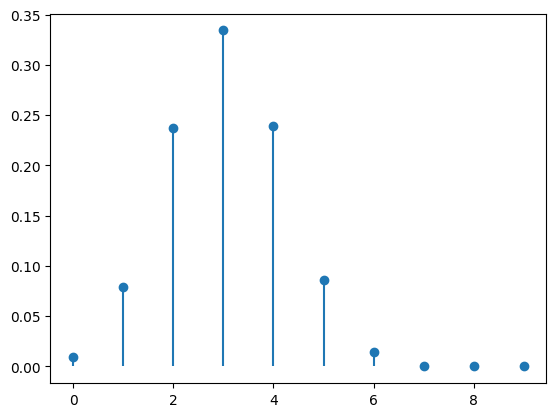
\includegraphics{images/hyp_pmf.png}
    }
}
    \caption{Rappresentazione grafica di una variabile aleatoria ipergeometrica $X \sim \mathcal H{(n, \, M, \, N)}$}
    \label{fig:mod_hyp}
    \vspace{\abovedisplayskip}
\end{figure}

\paragraph{Massa di probabilità} La funzione di massa di probabilità si ottiene tramite il rapporto tra il numero di casi favorevoli e numero di casi possibili (principio fondamentale del calcolo combinatorio).

\[
\boxed{
p_X(i) = \frac{\dbinom{N}{i} \dbinom{M}{n-i}}{\dbinom{N+M}{n}} I_{\{0, \, \dots, \, n \}}(i)
}
\]

\begin{itemize}
    \item $\dbinom{N}{i}$ = Numero di modi con cui posso estrarre $i$ oggetti funzionanti;
    \item $\dbinom{M}{n-i}$ = Numero di modi con cui posso estrarre $n - i$ oggetti difettosi;
    \item $\dbinom{N+M}{n}$ = Numero di modi con cui posso estrarre $n$ oggetti in generale.
\end{itemize}

\paragraph{Valore atteso}
Come per il modello binomiale, il calcolo del valore atteso può essere fatto scomponendo la variabile aleatoria $X$ in $n$ variabili aleatorie $X_i \sim \mathcal B$; l'$i$-esima variabile aleatoria vale $1$ se l'$i$-esimo oggetto è funzionante, $0$ altrimenti.
\begin{align*}
    \mathbb{E}(X_i) &= P(X_i = 1) = \frac{N}{N + M} = p \\
    \mathbb{E}(X) &= \mathbb{E}\left(\sum_{i=0}^n X_i\right) = \sum_{i=0}^n \mathbb{E}(X_i) = \sum_{i=0}^n p = np = n \frac{N}{N + M}
\end{align*}

\noindent Questi risultati sono generici perché non posso dire nulla sulle estrazioni 

\paragraph{Varianza}
Utilizzando la scomposizione fatta prima calcoliamo la varianza; importante notare che qua esperimenti consecutivi sono \textbf{dipendenti}, quindi nel calcolo della varianza si deve tenere conto anche della covarianza.
\begin{align*}
\operatorname{Var}(X_i) &= p(1-p) = \frac{N}{N + M} \left( \frac{N + M - N}{N + M}\right) = \frac{M N}{(N+M)^2} \\
\operatorname{Cov}(X_i, \, X_j) &= \mathbb{E}(X_i X_j) - \mathbb{E}(X_i) \mathbb{E}(X_j) = P(X_i = 1 \wedge X_j = 1) - P(X_i = 1) P(X_j = 1)
\end{align*}

\noindent $X_i \text{ e } X_j$ sono variabili di Bernoulli, quindi anche la somma lo è. \\ Non possiamo fattorizzare la prima probabilità, quindi la dobbiamo calcolare in un altro modo. \\
Considerando $i$ e $j$ tali che l'esperimento $j$-esimo avviene dopo l'esperimento $i$-esimo, allora
$$
P(X_i) = \frac{N}{N+M} \textnormal{, mentre } P(X_j) = \frac{N - 1}{N + M - 1}.
$$
Possiamo ora terminare il calcolo della covarianza di $X_i$:
\begin{align*}
    &= \frac{N}{N + M} \cdot \frac{N - 1}{N + M - 1} - \frac{N^2}{(N + M)^2} \\ 
    &= \frac{N}{N + M} \left( \frac{N-1}{N + M - 1} - \frac{N}{N + M} \right) \\
    &= \frac{N}{N + M} \left( \frac{(N-1)(N+M) - N(N+M-1)}{(N+M)(N+M-1)} \right) \\
    &= \frac{N}{N + M} \left( \frac{N^2 + NM - N - M - N^2 -NM + N)}{(N+M)(N+M-1)} \right) \\
    &= \frac{N}{N + M} \left( - \frac{M}{(N+M)(N+M-1)} \right) \\ 
    &= - \frac{NM}{(N+M)^2 (N + M - 1)}.
\end{align*}
Calcoliamo finalmente la varianza:
\begin{align*}
    \operatorname{Var}(X) &= \operatorname{Var}\left(\sum_{i=0}^{n} X_i\right) = \sum_{i=0}^n \operatorname{Var}(X_i) + \sum_{i \neq j} \operatorname{Cov}(X_i, X_j) = \\ 
    &= n \frac{NM}{(N + M)^2} - n(n-1) \frac{NM}{(N + M)^2 (N + M - 1)} = \\
    &= \frac{nNM}{(N + M)^2} \left( 1 - \frac{n-1}{N + M - 1} \right ) = n \cdot \frac{N}{N + M} \cdot \frac{M}{N + M} \left( 1 - \frac{n-1}{N + M - 1} \right ) = \\
    &= n p (1-p) \left( 1 - \frac{n-1}{N + M - 1} \right ).
\end{align*}
Notiamo come $np(1-p)$ sia la varianza del modello binomiale. \\
Considerando il caso in cui $N + M$ sia molto grande, tendente a $\infty$, e il numero delle estrazioni sia piccolo, possiamo dire che $1 - \frac{n-1}{N + M - 1*}$ sia molto vicino a $1$, di conseguenza la varianza del modello ipergeometrico è riconducibile alla varianza del modello binomiale.
Se invece il numero di estrazioni che posso fare è altissimo, l'universo degli elementi da cui estraggo cambierà molto poco, di conseguenza possiamo approssimare il modello ipergeometrico con il modello binomiale

\subsubsection{Modello esponenziale $X \sim E{(\lambda)}$}
\begin{figure}[h]
    \centering
\subfloat[Funzione di densità di probabilità]{
    \resizebox{7cm}{!}{
        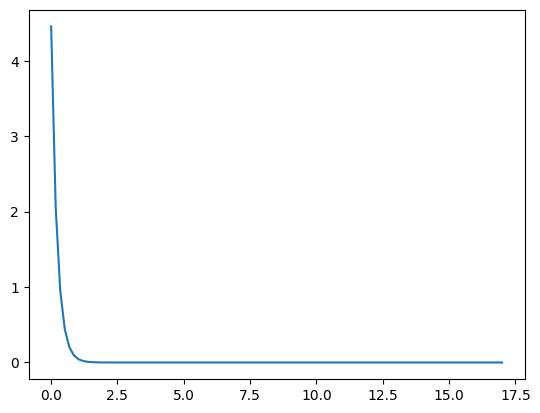
\includegraphics{images/expon_pdf.png}
    }
}
\subfloat[Funzione di ripartizione]{
    \resizebox{7cm}{!}{
        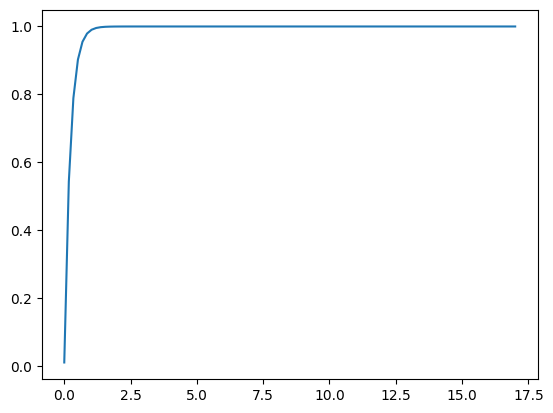
\includegraphics{images/expon_cdf.png}
    }
}
    \caption{Rappresentazione grafica di una variabile aleatoria esponenziale $X \sim E{(\lambda)}$}
    \label{fig:mod_expon}
    \vspace{\abovedisplayskip}
\end{figure}

Il modello esponenziale è una distribuzione di probabilità continua che descrive il tempo di attesa tra eventi in un processo di Poisson. Il parametro $\lambda$ controlla la forma della distribuzione esponenziale; più alto è il valore di $\lambda$ e più rapido è il decadimento della probabilità. In altre parole, un valore maggiore significa tempi di attesa più brevi tra gli eventi. Questo modello trova applicazioni in una varietà di contesti, come la modellizzazione del tempo tra arrivi di clienti in un sistema di code, la modellizzazione dei tempi di vita di dispositivi elettronici e altro ancora (per tempo non si parla di un valore atomico, in secondi, ma di un valore reale).
\newline \newline
Per capire se una variabile aleatoria segue un modello esponenziale, puoi esaminare il suo grafico e cercare alcune caratteristiche chiave associate a questa distribuzione:
\begin{itemize}
    \item La distribuzione esponenziale ha una forma specifica nel suo grafico di probabilità o densità di probabilità. Il grafico è caratterizzato da una coda lunga nella direzione positiva (a destra) rispetto al picco della distribuzione. Quindi, cerca una coda lunga sulla destra.
    \item Un indicatore importante è la presenza di un decadimento esponenziale. Questo significa che la probabilità di ottenere valori più grandi diminuisce in modo esponenziale all'aumentare del valore. Puoi osservare questa caratteristica nel grafico.
\end{itemize}

\paragraph{Densità di probabilità} Una variabile aleatoria $X$, avente un supporto $D_X = [0, +\infty)$, si dice seguire il modello esponenziale se, dato un $\lambda \in (0, +\infty)$:
$$
\boxed{
f_X(x) = \lambda e^{-\lambda x} \cdot I_{[0, +\infty)}(x)
}.
$$
Verifichiamo che l'integrale della funzione di densità di probabilità sia 1:
\begin{align*}
    \int_{-\infty}^{+\infty} f_X(x) dx &= \int_{0}^{+\infty} \lambda e^{-\lambda x} dx 
    \intertext{sostituiamo $\displaystyle u = \lambda x$ ottenendo $du = \lambda dx$:}
    &= \int_{0}^{+\infty} \lambda e^{-u} \frac{du}{\lambda} \\
    &= \int_{0}^{+\infty} e^{-u} du \\ 
    &= \left [ -e^{-u} \right ]_{0}^{+\infty} \\ 
    &=-e^{-\infty} + e^{0} = 0 + 1 = 1.
\end{align*}
Anche in questo caso, la \textbf{rapidità} del \textit{decadimento esponenziale} dipende dal valore di $\lambda$. \\
Si noti che $e^{-x}$ per $x \rightarrow \infty$ tende a $0$, quindi $-e^{-\infty} = -0 = 0$.

\paragraph{Funzione di ripartizione}
Per calcolare la funzione di ripartizione, integriamo da $-\infty$ a $x$:
\begin{align*}
    F_X(x) &= P(X \leq x) = \int_{-\infty}^{x} f_X(u) du \\
    &= \int_{0}^{x} \lambda e^{-\lambda u} du
    \intertext{come prima, sostituiamo $\displaystyle t = \lambda u$, cambiando gli estremi di integrazione:}
    &= \int_{0}^{\lambda x} \lambda e^{-t} \frac{dt}{\lambda} \\
    &= \int_{0}^{\lambda x} e^{-t} dt  \\
    &= \left[ -e^{-t} \right ]_{0}^{\lambda x} \\
    &= -e^{-\lambda x} + e^0 \\
    &= (1 - e^{-\lambda x}) I_{[0, +\infty)}(x).
\end{align*}
In questo caso, il valore di $\lambda$ determina la \textit{rapidità} della salita esponenziale della funzione di ripartizione.

\paragraph{Valore atteso}
\begin{align*}
    \mathbb E(X) &= \int_{-\infty}^{+\infty} x f_X(x) dx = \int_{0}^{+\infty} x \lambda e^{-\lambda x} dx =
    \intertext{integriamo per parti con $f(x) = x$ e $g'(x) = \lambda e^{-\lambda x}$:}
    &= \left [ -x e^{-\lambda x} \right ]_{0}^{+\infty} - \int_{0}^{+\infty} -e^{-\lambda x} dx = \\ 
    &= 0 +  \int_{0}^{+\infty} e^{-\lambda x} dx = \\
    &= \frac{1}{\lambda} \int_{0}^{+\infty} \lambda e^{-\lambda x} dx = \\ 
    &= \frac{1}{\lambda} \underbrace{\int_{0}^{+\infty} f_X(x) dx}_{= 1} = \frac{1}{\lambda}.
\end{align*}

\paragraph{Varianza}
Per calcolare la varianza, utilizziamo la formula alternativa $\operatorname{Var}(X) = \E(X^2) - \E(X)^2$:
\begin{align*}
    \mathbb E(X^2) &= \int_{-\infty}^{+\infty} x^2 f_X(x) dx = \int_{0}^{+\infty} x^2 \lambda e^{-\lambda x} dx =
    \intertext{integriamo per parti con $f(x) = x^2$ e $g'(x) = \lambda e^{-\lambda x}$:}
    &= \left [ -x^2 e^{-\lambda x} \right]_{0}^{+\infty} - \int_{0}^{+\infty} -2x e^{-\lambda x} dx =
    \intertext{valutiamo la prima funzione e aggiungiamo (moltiplicando e dividendo) un $\displaystyle \lambda$ nell'integrale:}
    &= 0 + \frac{2}{\lambda} \underbrace{\int_{0}^{+\infty} \lambda x e^{-\lambda x} dx}_{= \mathbb E(X)} = \frac{2}{\lambda} \cdot \frac{1}{\lambda} = \frac{2}{\lambda^2}.
\end{align*}
Per concludere, la varianza: \[
    \operatorname{Var}(X) = \mathbb E(X^2) - \mathbb E(X)^2 = \frac{2}{\lambda^2} - \frac{1}{\lambda^2} = \frac{1}{\lambda^2}.
\]

\paragraph{Assenza di memoria}
Il modello esponenziale è l'unico modello continuo che gode dell'assenza di memoria:
$$
\boxed{
P(X > s + t \ | \ X > s) = P(X > t)
}.
$$
Il modello non tiene traccia dei dati passati o delle informazioni storiche. In altre parole, il modello non tiene conto dei valori precedenti o delle osservazioni precedenti. Questo approccio può essere utile in alcune situazioni in cui si desidera dare più peso alle informazioni più recenti o si ritiene che i dati passati non siano rilevanti per le previsioni future.

\begin{dimostrazione}[Assenza di memoria del modello esponenziale]
\begin{align*}
    \dfrac{P( X > s + t \cap X > s)}{P(X > s)} = P(X > t) \\
    P(X > s + t \cap X > s) = P(X > t)P(X > s) \\
    \intertext{sapendo che $P(X > x) = 1 - P(X \leq x) = 1 - F_X(x) = 1 - (1 - e^{-\lambda x}) = e^{-\lambda x}$, quindi:}
    P(X > s + t) = P(X > t) P(X > s) \\ 
    \Longrightarrow e^{-\lambda (s+t)} = e^{-\lambda t} e^{-\lambda s}
    \tag*{$\blacksquare$}
\end{align*}
\end{dimostrazione}

\paragraph{Scalatura}
Cosa succede se andiamo a scalare una variabile aleatoria $X \sim E{(\lambda)}$?
Definiamo $Y := \alpha X$ con $\alpha > 0$ e cerchiamo il modello di distribuzione che segue $Y$; per far ciò, dimostriamo che la funzione di ripartizione $F_Y(x)$ è uguale a quella di qualche modello di distribuzione che già conosciamo. Infatti, la funzione di ripartizione definisce in modo completo tutto il modello. Cerchiamo quindi la definizione analitica di $F_Y(x)$:
\begin{align*}
    F_Y(x) &= P(Y \leq x) = P(\alpha X \leq x) = P\left(X \leq \frac{x}{\alpha}\right) = F_X\left(\frac{x}{\alpha}\right) = \\
    &= 1 - e^{-\frac{x}{\alpha} \lambda} = 1 - e^{-\frac{\lambda}{\alpha} x} = 
    \intertext{sia $\displaystyle \frac{\lambda}{\alpha} = \lambda'$, quindi}
    &= 1 - e^{-\lambda' x}.
\end{align*}
Abbiamo dimostrato che la funzione di ripartizione di $Y$ è uguale a quella di una variabile aleatoria che segue un modello esponenziale, quindi $Y \sim E{(\lambda')}$.
È importante ricordare che due variabili aleatorie con la stessa funzione di ripartizione seguono lo stesso modello (anche se hanno parametri diffrenti)

\paragraph{Massimo e minimo di una serie di variabili aleatorie}
Siano $X_1, \, \dots ,\, X_n$ variabili aleatorie, siamo interessati al minimo valore assunto da queste $n$ variabili aleatorie: definiamo quindi $Y := \min\{{X_1, \, \dots \, X_n\}}$. Tentiamo di calcolare quale valore assume $P(Y > x)$ per un certo $x$, aggiungendo mano a mano delle assunzioni.
Innanzitutto, verificare che il minimo di $X_1, \, \dots, \, X_n$ sia maggiore di un valore $x$ significa verificare che tutti i valori siano maggiori di $x$.
\begin{align*}
    P(Y > x) &= P(\min\{{X_1, \, \dots, \, X_n\}} > x) = P(\forall i \: X_i > x) = P \left (\bigcap_{i=1}^n \{X_i > x\} \right ) =
    \intertext{assumiamo che le variabili aleatorie siano indipendenti:}
    &= \prod_{i=1}^n P(X_i > x) = \prod_{i=1}^n (1 - F_{X_i}(x)) =
    \intertext{assumiamo che le variabili aleatorie siano \textbf{i.i.d.}\ (\textit{indipendenti e identicamente distribuite}):}
    &= \prod_{i=1}^n (1 - F_X(x)) = (1 - F_X(x))^n =
    \intertext{assumiamo che le variabili aleatorie seguano un modello esponenziale $E{(\lambda)}$:}
    &= (1 - (1 - e^{-\lambda x}))^n = (e^{-\lambda x})^n = e^{-n \lambda x} =
    \intertext{sostituiamo $n \lambda = \lambda'$:}
    F_Y(x) &= P(Y \leq x) = 1 - P(Y > x) = 1 - e^{-\lambda' x}.
\end{align*}
Abbiamo quindi dimostrato che $Y \sim E{(\lambda')}$. \\ \\
Per rendere ancora più generale la dimostrazione, assumiamo che $X_i \sim E{(\lambda_i)}$:
\begin{align*}
    \prod_{i = 1}^n (1 - F_{X_i}(x)) &= \prod_{i = 1}^n (1 - (1 - e^{-\lambda_i x})) = \prod_{i = 1}^n e^{-\lambda_i x} = \\
    &= e^{\displaystyle \sum_{i=1}^n -\lambda_i x} = e^{\displaystyle x \sum_{i=1}^n -\lambda_i} =
    \intertext{sostituiamo $\displaystyle \sum_{i=1}^n -\lambda_i = \lambda''$:}
    F_Y(x) &= 1 - e^{\lambda'' x}.
\end{align*}
Quindi anche se ogni variabile aleatoria $X_i$ ha un proprio parametro $\lambda_i$ la dimostrazione vale. \\ \\
È possibile fare le stesse assunzioni anche per $Y := \max\{{X_1, \, \dots \, X_n\}}$:
\begin{align*}
    F_Y(x) &= P(Y \leq x) = P(\max\{{X_1, \, \dots \, X_n\} \leq x}) = P(\forall i \: X_i \leq x) = P \left( \bigcap_{i=1}^n \{X_i \leq x\} \right )
    \intertext{assumiamo che le variabili aleatorie siano indipendenti:}
    &= \prod_{i=1}^n P(X_i \leq x) = \prod_{i=1}^n F_{X_i}(x)
    \intertext{assumiamo infine che le variabili aleatorie siano identicamente distribuite:}
    &= \prod_{i=1}^n F_X(x) = \left ( F_X(x) \right )^n.
\end{align*}

\subsubsection{Modello Gaussiano o normale $X \sim N(\mu, \sigma)$}
\begin{figure}[h]
    \centering
\subfloat[Funzione di densità di probabilità]{
    \resizebox{7cm}{!}{
        \begin{tikzpicture}
        \begin{axis}[
            clip=false,
            enlargelimits=false,
            %axis lines = center,
            %axis equal,
            xlabel = $x$,
            ylabel = $f_X$,
            %ymin=0, ymax=1.1,
            %xmin=0, xmax=4,
            samples=100,
            ytick = {0,1},
            %xtick = {1},
            %yticklabels={$\dfrac 13$, 1},
            xtick={0},
            xticklabels={$\mu$},
            %yticklabels={1},
            domain={-4:4},
            %extra x ticks={0},
        ]
        \addplot[color=blue, thick]{1/(sqrt(2*pi))*e^(-(x^2/2))};
        \end{axis}
        
        \end{tikzpicture}
    }
}
\subfloat[Funzione di ripartizione]{
    \resizebox{7cm}{!}{
        \begin{tikzpicture}
        \begin{axis}[
            clip = false,
            enlargelimits=false,
            axis lines = center,
            %axis equal,
            xlabel = $x$,
            ylabel = $F_X$,
            domain={-4:4},
            samples=100,
            %ymin=0, ymax=1.1,
            %xmin=0, xmax=4,
            ytick = {1/2, 1},
            %yticklabels={$\dfrac 13$, $\dfrac 23$, 1},
            %xtick={1,2,3},
            xtick={0},
            %xticklabels={$\mu$},
            ymax=1,
            extra x ticks={0},
            extra x tick labels={$\mu$},
            extra y ticks={1},
        ]
        \addplot[color=blue, thick]{
        (e^(2*x*sqrt(2/pi)))/(1+e^(2*x*sqrt(2/pi)))
        };

        \end{axis}
        \end{tikzpicture}
    }
}
    \caption{Rappresentazione grafica di una variabile aleatoria normale $X \sim N{(\mu, \, \sigma)}$}
    \label{fig:mod_gauss}
\end{figure}

\noindent La distribuzione normale, o gaussiana, è utilizzata per modellare variabili continue in molteplici contesti, grazie alla sua forma a campana simmetrica e alle proprietà ben note.
\newline \newline
Per capire se una distribuzione di dati segue il modello normale (distribuzione gaussiana), puoi utilizzare diverse tecniche di analisi grafica. Ecco alcuni metodi comuni:
\begin{itemize}
    \item Un istogramma rappresenta la distribuzione dei dati in barre verticali. Nella distribuzione normale, l'istogramma ha una forma a campana simmetrica con la media, la mediana e la moda che coincidono. Puoi confrontare l'istogramma con una curva teorica normale per valutare l'adattamento.
    \item Se i punti nel Q-Q plot seguono approssimativamente una linea retta, i dati sono consistenti con una distribuzione normale. Deviazioni dalla retta indicano deviazioni dalla normalità.
    \item Puoi creare un grafico della densità di probabilità dei dati, che rappresenta graficamente la distribuzione di probabilità teorica dei dati in base a una distribuzione normale con media e deviazione standard stimati. Se la curva teorica si adatta bene ai dati, questo può suggerire una distribuzione normale.
    \item  Un box plot può aiutare a visualizzare la simmetria e la presenza di outlier nei dati. Una distribuzione normale generalmente produce un box plot con una mediana al centro della "scatola" e valori outlier limitati.
\end{itemize}

\paragraph{Densità di probabilità}
Una variabile aleatoria $X$, avente supporto $D_X = \{ \mathbb R \}$, si dice seguire il modello gaussiano (anche detto \textit{normale}) se, dato un $\sigma > 0, \, \text{con} \, \sigma^2 \in \left(0, +\infty\right)$ e un $\mu \in \mathbb R$ allora:
\[
\boxed{
f_X(x) = \frac{1}{\sqrt{2 \pi} \sigma} \exp{\!\left(-\frac{(x-\mu)^2}{2\sigma^2} \right)}
}.
\]

Lo studio della funzione è il seguente:
\begin{itemize}
    \item dominio: $\mathbb R$;
    \item codominio: $\mathbb R^+$;
    \item limiti: $\lim\limits_{x \to \infty} f_X(x) = 0^+$;
    \item asintoti: orizzontale $y = 0$, no verticali e obliqui;
    \item simmetrie: simmetrica rispetto a $x = \mu$;
    \item derivata prima: $\displaystyle f'_X(x) = \frac{1}{\sqrt{2 \pi} \sigma^3} \exp{\!\left(-\frac{(x-\mu)^2}{2\sigma^2} \right)} (\mu - x)$;
    \item monotonia: cresce per $x < \mu$, decresce per $x > \mu$ e ha un massimo in $x = \mu$;
    \item derivata seconda: $\displaystyle f''_X(x) = \frac{1}{\sqrt{2 \pi} \sigma^3} \exp{\!\left(-\frac{(x-\mu)^2}{2\sigma^2} \right)} \left ( \frac{(x - \mu)^2}{\sigma^2} - 1 \right )$;
    \item concavità: $x < \mu - \sigma \lor x > \mu + \sigma$ verso l'alto, $\mu - \sigma < x < \mu + \sigma$ verso il basso, flessi in $x = \mu \pm \sigma$.
\end{itemize}
$\mu$ definisce la centralità della distribuzione, mentre $\sigma$ la dispersione. \\ 

\begin{dimostrazione}[La funzione di densità della distribuzione normale integra a 1]
\begin{align*}
    \int_{-\infty}^{+\infty} f_X(x) dx &= \int_{-\infty}^{+\infty} \frac{1}{\sqrt{2 \pi} \sigma} \exp{\!\left(-\frac{(x-\mu)^2}{2\sigma^2} \right)} =
    \intertext{sostituiamo $y = \dfrac{x - \mu}{\sigma}$, ponendo $dy = \dfrac{dx}{\sigma}$:}
    &= \int_{-\infty}^{+\infty} \frac{1}{\sqrt{2 \pi}} \exp{\left(\frac{1}{2} y^2 \right)} dy = \frac{1}{\sqrt{2 \pi}} \int_{-\infty}^{+\infty} \exp{\left(\frac{1}{2} y^2 \right)} dy = 1.
    \intertext{chiamando $I$ l'integrale, allora $I = \sqrt{2 \pi} \Longrightarrow I^2 = 2\pi$:}
    I \cdot I = 2\pi & \Longrightarrow \int_{-\infty}^{+\infty} \exp{\left(\frac{1}{2} x^2 \right)} dx \int_{-\infty}^{+\infty} \exp{\left(\frac{1}{2} y^2 \right)} dy = 2 \pi
    \intertext{concentriamoci solo sul doppio integrale:}
    & \int_{\mathbb R} \int_{\mathbb R} \left ( \exp{\left(\frac{1}{2} x^2 \right)} \cdot \exp{\left(\frac{1}{2} y^2 \right)} \right ) dx dy = \int_{\mathbb R} \int_{\mathbb R} \left ( \exp{\left(\frac{1}{2} (x^2 + y^2) \right)} \right ) dx dy
    \intertext{passiamo alle coordinate polari:}
    &= \int_{0}^{2\pi} \int_{0}^{+\infty} p \exp{\left(\frac{1}{2} p^2 \right)} dp d\theta = \underbrace{\int_{0}^{2\pi} 1 d\theta}_{= 2\pi} \int_{0}^{+\infty} \exp{\left(\frac{1}{2} p^2 \right)dp}
    \intertext{chiamando $S$ il secondo integrale, abbiamo ottenuto $2\pi \cdot S = 2 \pi$; dimostriamo allora che $S = 1$ effettuando un cambio di variabile $r = \frac{1}{2}p^2$ con $dr = p \cdot dp$:}
    \int_{0}^{+\infty} \exp{\left(\frac{1}{2} p^2 \right)} &= \int_{0}^{+\infty} e^{-r} dr = \int_{0}^{+\infty} (1) \cdot e^{(-1)r} dr
    \intertext{l'integrale contiene la funzione di densità di probabilità di una v.a. aleatoria esponenziale di parametro $1$, che ovviamente integra a $1$.}
\end{align*}
\end{dimostrazione}



\paragraph{Funzione di ripartizione}
La funzione di ripartizione di una v.a.\ normale è molto complicata poiché
$$
F_X(x) = \int_{-\infty}^{x} f_X(v) dv = \int_{-\infty}^{x} \frac{1}{\sqrt{2 \pi} \sigma} \exp{\!\left(-\frac{(v-\mu)^2}{2\sigma^2} \right) dv}
$$
non ha una formula analitica.

\paragraph{Valore atteso}
$$
\E(X) = \mu
$$

\paragraph{Varianza}
$$
\operatorname{Var}(X) = \sigma^2
$$

\paragraph{Trasformazioni lineari}
Definiamo $Y := aX + b$ con $a,b \in \mathbb R$ e calcoliamo il valore atteso e la varianza:
\begin{align*}
    \E(Y) &= \E(aX + b) \\
    &= a \E(X) + b \\ 
    &= a\mu + b; \\
%\end{align*}
%\begin{align*}
    \operatorname{Var}(Y) &= \operatorname{Var}(aX + b) \\ 
    &= a^2 \operatorname{Var}(X) + 0 \\ 
    &= a^2 \sigma^2.
\end{align*}
Osserviamo quindi come $Y := aX + b$ è una variabile aleatoria normale di parametri $N{(a\mu + b, \, |a|\sigma)}$.

\paragraph{Standardizzazione}
Data una variabile aleatoria $X \sim N(\mu, \, \sigma)$ si definisce \[
\mathcal Z := \displaystyle \frac{X - \mu}{\sigma} \sim N{\displaystyle \left (\cancel{\frac{1}{\sigma} \mu - \frac{\mu}{\sigma}}, \, {\frac{1}{\cancel \sigma} \cancel \sigma} \right )} = N{(0, \, 1)} 
\] ottenendo una variabile aleatoria normale con parametri $\mathcal Z \sim N{(0, \, 1)}$, denominata \textbf{normale standard}. \\
Quest'ultima forma può essere utile per calcolare la funzione di ripartizione $F_X(x)$ di una variabile aleatoria normale generica $X \sim N{(\mu, \, \sigma)}$, in termini della normale standard $\mathcal Z$:
$$
    F_X(x) = P(X \leq x) = P \left (\frac{X - \mu}{\sigma} \leq \frac{x - \mu}{\sigma} \right ) = P \left (\mathcal Z \leq \frac{x - \mu}{\sigma} \right ) \! \! .
$$

% Figura gauss phi
\begin{figure}[ht]
\centering
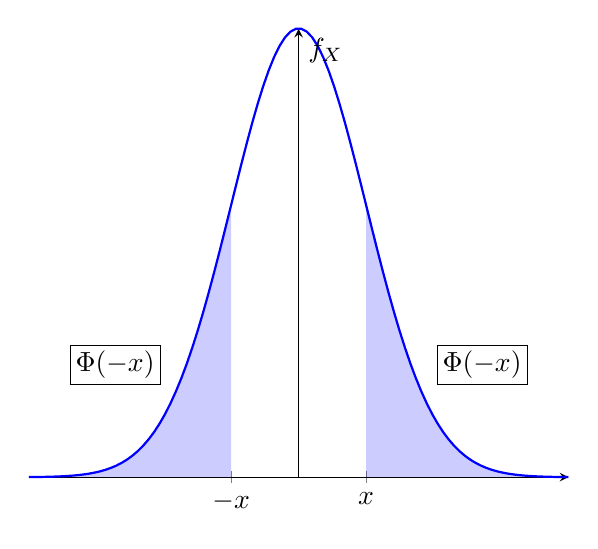
\begin{tikzpicture}
\begin{axis}[
    clip=false,
    enlargelimits=false,
    axis lines = center,
    %axis equal,
    %xlabel = $x$,
    ylabel = $f_X$,
    %ymin=0, ymax=1.1,
    %xmin=0, xmax=4,
    samples=100,
    ytick = {0,1},
    %xtick = {1},
    %yticklabels={$\dfrac 13$, 1},
    xtick={-1,1},
    xticklabels={$-x$, $x$},
    %yticklabels={1},
    domain={-4:4},
    %extra x ticks={0},
]
\addplot[name path=f, color=blue, thick]{1/(sqrt(2*pi))*e^(-(x^2/2))};
\path[name path=axis] (-4, 0) -- (4, 0);
\addplot [
    thick,
    color=blue,
    fill=blue, 
    fill opacity=0.2
    ] fill between[
    of=f and axis,
    soft clip={domain=-4:-1},
];
\addplot [
    thick,
    color=blue,
    fill=blue, 
    fill opacity=0.2
    ] fill between[
    of=f and axis,
    soft clip={domain=1:4},
];
\node[black, draw=black, inner sep=2pt] at (axis cs: -2.72, 0.1) {$\Phi(-x)$};
\node[black, draw=black, inner sep=2pt] at (axis cs: 2.72, 0.1) {$\Phi(-x)$};
\end{axis}
\end{tikzpicture}
\caption{Rappresentazione grafica di una normale standard, con l'area $\Phi(-x)$}
\label{fig:gauss_phi}
\end{figure}

\noindent Essendo $\frac{x - \mu}{\sigma}$ un valore numerico è possibile calcolare $F_X(x)$ utilizzando una tabella di una normale standard.
La funzione di ripartizione di una normale standard si indica con $\Phi(x)$. \\ Definiamo una relazione tra $\Phi(x)$ e $\Phi(-x)$, con $x > 0$:
\begin{align*}
    \Phi(-x) &= P(\mathcal Z \leq -x) \\
    &= P(\mathcal Z \geq x) \\
    &= 1 - P(\mathcal Z \leq x) \\
    &= 1 - \Phi(x) \\
\end{align*}

\noindent Le due aree evidenziate nel grafico di \figurename \ \ref{fig:gauss_phi} sono equivalenti. 
Calcolando $\Phi(-x)$ notiamo che è equivalente alla parte di grafico prima dell'area evidenziata a destra; essendo l'area complessiva 1 possiamo concludere che:
\[
\Phi(x) + \Phi(-x) = 1,
\]
quindi: \[
\Phi(-x) = 1 - \Phi(x).
\]

\paragraph{Indipendenza tra v.a.\ normali (riproducibilità)}
Siano $X_1 \sim N{(\mu_1, \, \sigma_1)}$ e $X_2 \sim N{(\mu_2, \, \sigma_2)}$ due v.a.\ normali indipendenti, allora \[
X_1 + X_2 \sim N{\left(\mu_1 + \mu_2, \, \sqrt{\sigma_1^2 + \sigma_2 ^2}\right)}.\]
Questa proprietà si estende a $n$ variabili aleatorie normali \textbf{indipendenti}.
\newline \newline
Siccome una variabile aleatoria binomiale non è altro che una somma di variabili aleatorie di Bernoulli, allora per un numero $n$ abbastanza grande è possibile approssimare la variabile aleatoria a una normale di parametri $\mu = np$ e $\sigma = \sqrt{np(1-p)}$.
\newline \newline
Per trovare l'ultimo valore sensato dell'asso delle ascisse, basta applicare la funzione di ripartizione inversa \textbf{ppf}$(0.99)$ alla variabile aleatoria per trovare il quantile che corrisponde al livello $0.99$.

\begin{landscape}
\setcellgapes{4pt}
\begin{table}[p]
\makegapedcells
\centering
\caption*{{Tabella 1}: Riassunto dei modelli di distribuzione}
\begin{tabular}{r|l||c|c|c|c}
    \makecell[r]{\textbf{\textit{Modello}}} & \textbf{\textit{Parametri}} & \textbf{\textit{F. di massa o di densità}}& \textbf{\textit{Funzione di ripartizione}} & \textbf{\textit{Valore atteso}} & \textbf{\textit{Varianza}} \\
    \hline
    \textbf{Bernoulli} & $X \sim B{(p)}$ & $\displaystyle p^x(1-p)^{(1-x)} I_{\{0, \, 1\}}(x)$ & \phantom{$\displaystyle  \sum_{i=0}^{\lfloor x \rfloor}$} $(1-p)I_{[0, \, 1)}(x) + I_{[1, \, +\infty)}(x)$ \phantom{$\displaystyle  \sum_{i=0}^{\lfloor x \rfloor}$} & $p$ & $p(1-p)$ \\
    \hline
    \textbf{Binomiale} & $X \sim B{(n, \, p)}$ & $\displaystyle \binom{n}{x} p^x (1-p)^{n-x} I_{\{0, \, \dots, \, n\}}(x)$ & $\displaystyle  \sum_{i=0}^{\lfloor x \rfloor} \binom n i p^i(1-p)^{n-i} I_{[0, \, n]}(x) + I_{(n, \, +\infty)}(x)$ & $n p$ & $n p(1-p)$ \\
    \hline 
    \textbf{Uniforme discreto} & $X \sim U{(n)}$ & $\displaystyle \frac 1n I_{\{1, \, \dots, \, n\}}(x)$ & \phantom{$\displaystyle  \sum_{i=0}^{\lfloor x \rfloor}$} $\displaystyle \frac{\lfloor x \rfloor}{n} I_{[0, \, n]} + I_{(n, \, +\infty)}(x)$ \phantom{$\displaystyle  \sum_{i=0}^{\lfloor x \rfloor}$} & $\displaystyle  \frac{n+1}2$ & $\displaystyle \frac{n^2-1}{12}$ \\
    \hline
    \textbf{Uniforme continuo} & $X \sim U{(a, \, b)}$ & $\displaystyle \frac{1}{b-a} I_{[a, \, b]}(x)$ & \phantom{$\displaystyle  \sum_{i=0}^{\lfloor x \rfloor}$} $\displaystyle \frac{x-a}{b-a} I_{[a, \, b]}(x) + I_{(b, \, +\infty)}(x)$ \phantom{$\displaystyle  \sum_{i=0}^{\lfloor x \rfloor}$} & $\displaystyle \frac{b+a}2$ & $\displaystyle \frac{(b-a)^2}{12}$ \\
    \hline 
    \textbf{Geometrico} & $X \sim G{(p)}$ & \phantom{$\displaystyle  \sum_{i=0}^{\lfloor x \rfloor}$} $p(1-p)^x I_{\{0, \, \dots, \, +\infty\}}(x)$ \phantom{$\displaystyle  \sum_{i=0}^{\lfloor x \rfloor}$} & $\displaystyle (1-(1-p)^{\lfloor x \rfloor + 1}) I_{[0, +\infty)}(x)$ & $\displaystyle \frac {1-p}p$ & $\displaystyle \frac{1-p}{p^2}$ \\
    \hline 
    \textbf{Poisson} & $X \sim P{(\lambda)}$ & $\displaystyle e^{-\lambda} \frac{\lambda^x}{x!} I_{\{0, \, \dots, \, +\infty\}}(x)$ & \phantom{$\displaystyle  \sum_{i=0}^{\lfloor x \rfloor}$} [\textit{non vista}] \phantom{$\displaystyle  \sum_{i=0}^{\lfloor x \rfloor}$} & $\displaystyle \lambda$ & $\lambda$ \\
    \hline \phantom{$\displaystyle  \sum_{i=0}^{\lfloor x \rfloor}$} 
    \textbf{Ipergeometrico} & $X \sim \mathcal H{(n, \, M, \, N)}$ & $\displaystyle \frac{\dbinom{N}{x} \dbinom{M}{n-x}}{{\dbinom {N+M}{n}}} I_{\{0, \, \dots, \, n\}}(x)$ & [\textit{non vista}] & $\displaystyle np$ con $p= n\frac {N}{N + M}$ & $\displaystyle np(1-p)\!\left(1 - \frac{n-1}{M+N-1}\right)$ \\
    \hline \phantom{$\displaystyle  \sum_{i=0}^{\lfloor x \rfloor}$}
    \textbf{Esponenziale} & $X \sim E{(\lambda)}$ & $\lambda e^{-\lambda x} I_{[0, +\infty)}(x)$ & $(1-e^{-\lambda x}) I_{[0, +\infty)}(x)$ & $\dfrac 1 \lambda$ & $\dfrac {1}{\lambda^2}$ \\
    \hline \phantom{$\displaystyle  \sum_{i=0}^{\lfloor x \rfloor}$}
    \textbf{Gauss} & $X \sim G{(\mu, \, \sigma)}$ & $\displaystyle \frac{1}{\sqrt{2 \pi} \sigma} \exp{\!\left(-\frac{(x-\mu)^2}{2\sigma^2} \right)}$ & $\displaystyle \int_{-\infty}^{x} \frac{1}{\sqrt{2 \pi} \sigma} \exp{\!\left(-\frac{(x-\mu)^2}{2\sigma^2} \right)}$ & $\mu$ & $\sigma^2$ 
\end{tabular}
\end{table}

\end{landscape}

\subsubsection{Teorema centrale del limite}
\begin{teorema}[Teorema centrale del limite]
Siano $X_1, \, \dots \, , X_n$ v.a.\ i.i.d.\ come $X$ con $\E(X) = \mu$ e $\operatorname{Var}(X) = \sigma^2$, allora: \[\sum_{i=1}^n X_i \ \dot{\sim} \ N{(n\mu, \,\sqrt{n} \sigma)}.\]
\end{teorema}

Questo teorema è molto importante perché permette di approssimare una qualsiasi serie di v.a.\ i.i.d.\ ad una variabile normale, considerando un errore minimo.
La comodità delle v.a.\ normali è quella di applicare la standardizzazione. La notazione $\dot \sim$ indica un'\textit{andamento approssimato} della v.a.\ rispetto a un modello.
$$
\frac{\displaystyle \sum_{i=1}^n X_i - n\mu}{\sqrt{n} \sigma} \ \dot{\sim} \ N{(0,\,1)}
$$
Ad esempio, se $X_i \sim B{(p)}$ e $X = \sum\limits_{i=1}^n X_i \sim B{(n, p)} $, allora $X \ \dot{\sim} \ N{\left (n \E(X_i), \, \sqrt{n \operatorname{Var}(X_i)} \right)} = N{\left (np, \, \sqrt{np(1-p)} \right )}$.

\noindent Abbiamo detto che questa è un'approssimazione, ma cosa possiamo dire della sua accuratezza? \\
Si può dimostrare che all'aumentare di $n$ l'accuratezza aumenta, infatti portando $n$ ad infinito sia il valore atteso che la varianza vanno ad infinito.
Per evitare ciò si può sfruttare la normalizzazione mostrata sopra, in questo modo il valore atteso diventa $0$ e la varianza $1$.

\paragraph{Mediana}
La mediana è una specificazione (non osservazione, nel contesto delle v.a non ha senso parlare di osservazioni) $m$ che la v.a.\ assume tale che $P(X \leq m) = P(X \geq m) = \frac{1}{2}$, ovvero è quella specificazione che divide in due la funzione di ripartizione. Ad esempio, la mediana di $\mathcal{Z}$ è $0$.

\paragraph{Diagrammi Q-Q}
Come già accennato in precedenza il concetto di quantile è definito anche per le v.a: sia $\chi_q$ il quantile $q$-esimo (con $q \in [0,1]$), allora deve valere $P(X \leq \chi_q) = q$ e $P(X \geq \chi_q) = 1 - q$.
Come trovare il valore $\chi_q$?
$$
P(X \leq \chi_q) = q \Longrightarrow F_X(\chi_q) = q \Longrightarrow F^{-1}_X(F_X(\chi_q)) = F_X^{-1}(q) \Longrightarrow \chi_q = F^{-1}_X(q).
$$ \\

Come per la mediana, esiste un parallelo con i diagrammi Q-Q, che servivano per verificare che, preso un campione a coppie (due colonne di un data-frame), questi contenessero dei dati estratti dalla stessa popolazione. Per farlo si calcolano alcuni quantili (ad esempio i percentili) dei dati per poi graficarli (sulle ascisse i quantili della prima colonna e sulle ordinate quelli della seconda).
A questo punto otteniamo un grafico in cui, se i punti stanno sulla bisettrice del primo e del terzo quadrante, allora indipendentemente dal quantile scelto, entrambi hanno lo stesso, si conseguenza la popolazione è la stessa. \\
A questo punto possiamo applicare questo ragionamento alle variabili aleatorie, ma con una piccola differenza, infatti:
$$
    \forall q \in [0, 1] \quad \chi_q^{X} = \chi_q^{Y} \iff X \sim Y \quad \textnormal{Hanno la tessa distribuzione}
$$

La cosa più interessante da fare però è fare in modo che un'asse faccia riferimento ai \textbf{quantili campionari}, ovvero quantili di un campione osservato, mentre l'altro si riferisca ai \textbf{quantili teorici}, cioè i quantili della distribuzione (ad esempio la normale).
In questo modo è possibile validare l'ipotesi che i dati osservati seguano una certa distribuzione, verificando il Q-Q plot.
È fondamentale però conoscere pienamente la distribuzione (ovvero conoscerne anche i parametri) per poter calcolare i quantili della distribuzione. \\
Solitamente la distribuzione usata di default è la normale standard; vedremo successivamente che la media campionaria stimi molto bene il valore atteso, necessario per standardizzare, di conseguenza se calcolo la media campionaria dei dati posso stimare il valore atteso della distribuzione (vedremo nei paragrafi successivi). 
\newpage
\section{Statistica inferenziale}
La statistica inferenziale è la parte di statistica che si occupa di trarre conclusioni dei dati, nel nostro caso esploreremo la \textbf{statistica inferenziale parametrica puntuale}.

\noindent Nell'ambito della statistica inferenziale, rappresentiamo una \textbf{popolazione} come una v.a.\ $X$ che segue una distribuzione $X \sim F(\theta)$. La variabile aleatoria rappresenta l'\textit{incertezza} che si ha nella scelta del campione: il campionamento \textbf{non ha un criterio deterministico} e quindi non è garantito che il sottoinsieme di individui interrogati sia sempre lo stesso e risponda allo stesso modo (si dice anche \textbf{campione aleatorio}). 
Il \textbf{campione} è un insieme di $n$ elementi (individui) $\{ x_1, \, x_2, \, \dots, \, x_n \}$ ognuno dei quali appartiene al dominio della variabile aleatoria $X$: $\forall i \: \  x_i \in D_X$.
Il campione può anche essere rappresentato come un'\textbf{insieme di variabili aleatorie} $\{ X_1, \, X_2, \, \dots, \, X_n \}$ indipendenti e identicamente distribuite come $X$; così facendo, è possibile fare considerazioni senza aver fatto nessuna misurazione (infatti osservare $X$ è come fare una prova senza sapere quale sarà l'esito). In questo caso quindi non si sta parlando di un insieme di osservazioni come abbiamo fatto all'inizio del corso, infatti la statistica inferenziale pone dei fondamenti teorici per la statistica descrittiva. Gli \textbf{elementi} (individui) che si estraggono dalla popolazione sono sottoposti a un certo processo di misurazione il cui esito è il valore $x_i$. Per esempio, se la popolazione sono gli studenti della statale e ogni volta che se ne presenta uno in via Golgi viene chiesto il numero di esami superati, l'elemento (individuo) è lo studente mentre il processo di misurazione è chiedere il numero di esami passati e il valore che corrisponde a $x_i$.
\newline \newline
Parametrica perché ipotizziamo di conoscere quasi tutto della variabile aleatoria a meno di \textbf{uno o più parametri}. Si sa che la distribuzione della variabile aleatoria rientra in una delle famiglie di modelli (per esempio quella binomiale) però non si conosce almeno uno dei parametri della distribuzione. Indichiamo $X \dot{\sim} F(\theta)$ dove $F$ indica una generica famiglia di distribuzioni e $\theta$ il parametro ignoto.
\newline \newline
\noindent Una \textbf{statistica} o \textbf{stimatore} è una funzione di variabili aleatorie $t : D_X^n \rightarrow \mathbb R$ che preso in input un campione $x_1, \, \dots, \, x_n$, ovvero un numero di specificazioni della variabile aleatoria $X$, restituisce in output una stima del parametro $\theta$ di $X$: \[
\boxed{
t(x_1, \, x_2, \, \dots, \, x_n) = \hat \theta \approx \theta 
}
\]
Se si passano un numero di variabili aleatorie estratte da un'unica popolazione $X$ come argomenti alla statistica invece delle specificazione, si ottiene una funzione che è essa stessa una variabile aleatoria e che rappresenta il valore che si ottiene come stima prima ancora di aver osservato gli elementi del campione. Le proprietà che si possono estrapolare valgono indipendentemente dal particolare campione osservato.
\[
\boxed{
T = t(X_1, \, \dots , \, X_n) = \hat{t} \approx \tau(\theta)}
\]
Il valore numerico $\hat{t}$ della statistica è un'approssimazione della quantità ignota della funzione $\tau(\theta)$, la quale rappresenta un'altra quantità di interesse che non si conosce perché dipende dal parametro $\theta$.
\newline \newline
L'obiettivo della {\textbf{statistica inferenziale parametrica puntuale}} è trovare il parametro $\theta$ o una funzione $\tau(\theta)$ del modello $F$. \textbf{Tutto è uno stimatore di tutto}.
\newline
Una \textbf{famiglia di stimatori} $T_n = T_1, \, \dots, \, T_m$ è una combinazione lineare di variabili casuali.
\\
Ma a cosa serve uno stimatore, e a come lo ricaviamo?
Vogliamo che lo stimatore sia il più preciso possibile, in modo da poter ricavare il parametro la quantità ignota e poter ricavare informazioni sulla popolazione.

\subsection{Proprietà degli stimatori}

\subsubsection{Assenza di deviazione o distorsione}
Data una statistica $t(X_1, \, \dots, \, X_n)$, allora \[
\boxed{
t \text{ è \textbf{non deviata} rispetto a } \tau(\theta) \Longleftrightarrow \E(t[X_1, \, \dots, \, X_n]) = \tau(\theta)
}
\]

\noindent Se $t$ è invece deviata, il suo \textbf{bias} si definisce come: \[
\boxed{b_{\tau(\theta)}(T) := \E(t(X_1, \, \dots, \, X_N)) - \tau(\theta)}
\]
Un esempio di stimatore che possiede la proprietà di assenza di deviazione è la media campionaria $\overline{X}$.
\newline
Data la proprietà di assenza di distorsione, dire che il valore atteso dalla statistica intesa come variabile aleatoria è uguale a quello che si vuole stimare, vuol dire che la centralità della variabile aleatoria è approssimativamente uguale al valore ignoto. I valori che si osserveranno, come specificazioni della variabile aleatoria che corrisponde alla statistica calcolata sul campione, si distribuiranno attorno al valore che non si conosce e che si vuole stimare $\tau(\theta)$. Con un campione sufficientemente grande, queste statistiche tendono a convergere al vero valore del parametro che si sta cercando di stimare.

\subsubsection{Consistenza in media quadratica}
Abbiamo definito l'assenza di deviazione, però questo non basta: sappiamo infatti che la statistica $T$ oscilla intorno al valore $\tau(\theta)$ che vogliamo stimare, ma non sappiamo \textit{quanto} oscilla. 
Per misurare l'\textit{``oscillazione"}, calcoliamo la varianza auspicando un valore molto piccolo. Ad esempio, per lo stimatore media campionaria $\overline{X}$:
\begin{align*}
    \operatorname{Var}(\overline{X}) &= \operatorname{Var} \biggl (\frac{1}{n} \sum_{i=1}^n X_i \biggr ) = \frac{1}{n^2} \sum_{i=1}^n \operatorname{Var}(X_i) \\
    &= \frac{1}{n^2} \sum_{i=1}^n \operatorname{Var}(X) = \frac{1}{n^2} n\operatorname{Var}(X) \\
    &=\frac{\operatorname{Var}(X)}{n}.
\end{align*}
Osserviamo come la varianza dipende dalla varianza di $X$ e dalla taglia $n$ del campione. 
In particolare, nel caso in cui $T$ non sia deviata, più $n$ è grande più è accurata la stima. \\

\noindent Formalizziamo questa procedura per renderla indipendente dal modello e dalla statistica usata.

\paragraph{Consistenza}
Dati una popolazione $X$, il campione $\{X_1, \, \dots \, , X_n\}$ e $\theta$ il parametro di $X$, chiamiamo $T_n$ la famiglia di stimatori che sono costituiti dalla funzione $t_n$ applicata a $n$ argomenti. \\
Definiamo l'$\operatorname{MSE}_{\tau(\theta)}(T_n)$ (Mean Squared Error) come il valore medio dell'errore quadratico:
\[
\boxed{
\operatorname{MSE}_{\tau(\theta)}(T_n) := \E \! \left[(T_n - \tau(\theta))^2 \right ]
}.
\]

\noindent Inoltre: \[
\boxed{
T_n è \text{ è \textbf{consistente in media quadratica} rispetto a } \tau(\theta) \Longleftrightarrow \lim_{n\rightarrow +\infty} \operatorname{MSE}_{\tau(\theta)} (T_n) = 0}.
\]
Usiamo l'$\operatorname{MSE}$ e non la varianza perchè quest'ultima non tiene conto del valore $\tau(\theta)$ che stiamo cercando di stimare.
\noindent Analiticamente, l'$\operatorname{MSE}$ può essere definito come:
\begin{align*}
    \operatorname{MSE}_{\tau(\theta)}(T_n) &= \E\left[(T_n - \tau(\theta))^2 \right ] = \E \left[( (T_n - \green{\E(T_n)}) + (\red{\E(T_n)} - \tau(\theta)))^2 \right ] \\
    &= \E \left[ (T_n - \E(T_n))^2 + 2(T_n - \E(T_n))(\E(T_n) - \tau(\theta)) + (\underbrace{\E(T_n) - \tau(\theta)}_{\E[\E(T_n)]=\E(T_n)})^2 \right ] \\
    &= \underbrace{\E \left[ (T_n - \E(T_n))^2 \right]}_{= \operatorname{Var}(T)} + \underbrace{2(\E(T_n) - \tau(\theta)) \underbrace{\E[\left (T_n - \E(T_n) \right)]}_{\E(T_n) - \E[\E(T_n)] = 0}}_{= 0} + \underbrace{\left(\E(T_n) - \tau(\theta) \right)^2}_{= \text{bias}^2} \\
    &= \operatorname{Var}(T_n) + b_{\tau(\theta)}(T_n)^2.
\end{align*}
Notiamo che se $T$ è non deviato allora l'$\operatorname{MSE}$ e la varianza coincidono, perché il bias vale $0$ nel caso di stimatore non distorto. \\
È importante dire che questo valore non è mai negativo, inoltre minore è il valore dell'$\operatorname{MSE}$ e meglio è (abbiamo un errore minore). \\
Nel caso in cui la taglia del campione non sia ben definita, non è possibile calcolare l'$\operatorname{MSE}$ perchè non è possibile portare $n$ ad $\infty$.

\paragraph{Consistenza debole}
Data una successione $T_1, \, \dots , \, T_n$, allora: \[
\boxed{
T_1, \, \dots , \, T_n \text{ è \textbf{debolmente consistente} rispetto a } \tau(\theta) \Longleftrightarrow \forall \varepsilon > 0 \lim_{n \to +\infty} P(\tau(\theta) - \varepsilon < T_n < \tau(\theta) + \varepsilon) = 1}.
\]

\noindent Riassumendo, fissato $\varepsilon$, all'aumentare di $n$ la stima di $T_n$ non si discosta mai più di $\varepsilon$ da $\tau(\theta)$. \\
Si può dimostrare che se una successione è consistente allora lo è anche debolmente.

\begin{dimostrazione}[Una successione consistente lo è anche debolmente]
Vogliamo calcolare la probabilità contenuta nel limite:
\begin{alignat*}{2}
    P(\tau(\theta) - \varepsilon < T_n < \tau(\theta) + \varepsilon) &= P(|T_n - \tau(\theta)| < \varepsilon) \\ 
    &= P((T_n - \tau(\theta))^2 < \varepsilon^2) \\
    \tag{Disuguaglianza di Markov}
    &= 1 - P((T_n - \tau(\theta))^2 \geq \varepsilon^2) 
        && \geq 1 - \frac{\E((T_n - \tau(\theta))^2)}{\varepsilon^2} \\
        &&&\geq 1 - \frac{\operatorname{MSE}_{\tau(\theta)}(T_n)}{\varepsilon^2}.
\end{alignat*}
Per $n \to +\infty$ allora $MSE \to 0$, quindi la probabilità $P(\tau(\theta) - \varepsilon < T_n < \tau(\theta) + \varepsilon)$ vale 1:\[
    \lim_{n \rightarrow +\infty} 1- \cancelto{0}{\frac{\operatorname{MSE}_{\tau(\theta)}(T_n)}{\varepsilon^2}} = 1. \tag*{$\blacksquare$}
\]
\end{dimostrazione}

\subsubsection{Metodo di massima verosimiglianza}

Il metodo di \textbf{massima verosimiglianza} è una tecnica utilizzata per stimare i parametri di un modello statistico basandosi sui dati osservati, a patto di conoscere la funzione di massa. Il concetto principale di questo metodo è cercare di trovare quei valori dei parametri del modello che rendono più probabile l'osservazione dei dati che abbiamo a disposizione.

\noindent Questo metodo è applicabile sia per le variabili aleatorie continue che per quelle discrete. Iniziamo con quelle discrete.
\\
\noindent Iniziamo considerando la popolazione $X \sim D(\theta)$ (in questo caso vi è un abuso di notazione, infatti con questa scrittura si vuole dire che $X$ è una variabile aleatoria che segue una certa distribuzione $D$ con parametro $\theta$), e il campione $X_1, X_2, \ldots, X_n$ ovvero delle variabili aleatorie discrete distribuite come $X$.

\noindent Sappiamo che $p_X$ è la funzione di massa di probabilità di $X$. Possiamo anche dire di conoscere tutte le funzioni di massa di probabilità congiunte per le variabili aleatorie $X_1, X_2, \ldots, X_n$. Sapendo che queste variabili aleatorie sono indipendenti, possiamo scrivere la funzione di massa di probabilità congiunta come:

\[
p_{X_1, \ldots, X_n}(x_1, \ldots, x_n) = \prod_{i=1}^{n} P(X_i = x_i) = \prod_{i=1}^{n} p_X(x_i) = \ell(\theta)
\]

\noindent A questo punto, l'unica cosa che non conosciamo è $\theta$, poiché, avendo a disposizione le osservazioni rilevate tramite l'esperimento, conosciamo tutte le $x_i$.

\noindent Di conseguenza, provando per tutti i valori possibili di $\theta$, vogliamo trovare il valore che massimizza $\ell(\theta)$, ovvero:

\[
\hat{\theta} = \underset{\theta}{\operatorname{argmax}} \, \ell(\theta)
\]
\noindent Ma come si massimizza la funzione di verosimiglianza? Nel nostro caso basta annullare la derivata prima, ovvero porla uguale a $0$, il che significa trovare il \textbf{punto stazionario} (questa operazione è fattibile sotto certe ipotesi che non vedremo, ma che nel nostro caso vengono rispettate).
\\ \\
\noindent Molto spesso, però, al posto di massimizzare la funzione di verosimiglianza, si massimizza il logaritmo naturale di essa.
\\
Il motivo principale per cui si preferisce massimizzare il logaritmo naturale della funzione di verosimiglianza è dovuto a al fatto che essa è un prodotto di densità di probabilità, quindi prendere il logaritmo trasforma il prodotto in una somma, che è molto più facile da differenziare e ottimizzare. Inoltre Massimizzare il logaritmo della verosimiglianza $\ell(\theta)$ produce le stesse stime dei parametri perché il logaritmo è una funzione \textbf{monotona crescente}.
    \[
    \ell(\theta) = \log \ell(\theta) = \log \left( \prod_{i=1}^{n} p_X(x_i; \theta) \right) = \sum_{i=1}^{n} \log p_X(x_i; \theta)
    \]

\begin{esempio}[Stimatore di massima verosimiglianza per la binomiale di parametro $p$]
Sia $X$ una variabile aleatoria che rappresenta la popolazione, sappiamo che $X\sim B(p)$. Inoltre dato il campione $X_1,\, X_2,\, ...,\, X_n$, ovvero delle variabili aleatorie distribuite come $X$, la cui funzione di massa di probabilità è $p_X = p(X = x) = p^2(1-p)^{1-x}$.
vogliamo trovare lo stimatore per ricavare $p$, ovvero $\hat{p}$.

\begin{align*}
    \ell(p) = \prod_{i=1}^n p_X(x_i) = \prod_{i=1}^n p^{x_i}(1-p)^{1-X_i} = p^{\sumi x_i}(1-p)^{\sumi 1 - x_i} \\
\end{align*}

a questo punto applichiamo il logaritmo naturale

\begin{align*}
    \ln{\ell(p)} = \underbrace{\sumi{x_i}}_{s} \ln{p} + \underbrace{\sumi{1 - x_i}}_{n-s} \ln{1-p} 
\end{align*}

a questo punto dobbiamo derivare ciò che abbiamo ottenuto

\begin{align*}
    \frac{d}{dp} \ln{\ell(p)} = \frac{d}{dp} \left( s \ln{p} + (n - s) \ln{(1 - p)} \right) = \\ = \frac{d}{dp} \left( s \ln{p}\right) + \frac{d}{dp} \left((n - s) \ln{(1 - p)} \right) = \\
    = s \frac{1}{p} + (n - s) \frac{1}{1 - p} \cdot (-1) = \frac{s}{p} - \frac{n - s}{1 - p}
\end{align*}

infine poniamo la derivata a $0$ per massimizzare, e ricaviamo $p$

\begin{align*}
    \frac{s}{p} - \frac{n - s}{1 - p} = 0 \\
    \frac{s}{p} = \frac{n - s}{1 - p} \\
    (1-p)s = p(n - s) \\
    s - \cancel{ps} = pn - \cancel{ps} \\
    s = pn \\
    p = \frac{s}{n}
\end{align*}

\noindent in questo modo abbiamo trovato che Il valore di $p$ che massimizza la funzione di verosimiglianza è la proporzione di successi nel campione, cioè:

$$\hat{p} = \frac{1}{n}\sum_{i=1}^n x_i$$

\noindent di conseguenza otteniamo che lo stimatore massima verosimiglianza $T$, per il parametro $p$ è la media dei $x_i$.
\end{esempio}

\begin{esempio}[Stimatore di massima verosimiglianza per la geometrica di parametro $p$]
Sia $X$ una variabile aleatoria che rappresenta la popolazione, sappiamo che $X\sim G(p)$. Inoltre dato il campione $X_1,\, X_2,\, ...,\, X_n$, ovvero delle variabili aleatorie distribuite come $X$, la cui funzione di massa di probabilità è $p_X = p(X = x) = (1-p)^{x}p$.
vogliamo trovare lo stimatore per ricavare $p$, ovvero $\hat{p}$. \\

\noindent la funzione di verosimiglianza è data da:
\[
\ell(p) = \prod_{i=1}^n (1-p)^{X_i}p = p^n (1 - p)^{\sumi x_i}
\]

\noindent applichiamo il logaritmo naturale:
\[
\ln \ell(p) = \ln \left( p^n (1 - p)^{\sumi x_i} \right) = n \ln p + \left( \sumi x_i \right) \ln (1 - p)
\]

\noindent calcoliamo la derivata rispetto a \( p \):
\begin{align*}
    \frac{d}{dp} \ln \ell(p) = \frac{d}{dp} \left( n \ln p + \left( \sumi x_i \right) \ln (1 - p) \right) = \\
    = \frac{d}{dp} \left( n \ln p \right) + \frac{d}{dp} \left( \left( \sumi x_i \right) \ln (1 - p) \right) = \\
    = n \frac{1}{p} + (-1) \frac{\sumi x_i}{1 - p} \\
    = \frac{n}{p} - \frac{\sumi x_i}{1 - p}
\end{align*}

\noindent impostando la derivata uguale a zero per trovare il massimo:
\[
\frac{n}{p} - \frac{\sumi 1 - p} = 0
\]

Risolvendo per \( p \):
\begin{align*}
    \frac{n}{p} = \frac{\sumi x_i}{1 - p} \\
    n (1 - p) = p \sumi x_i \\
    n - np = p \sumi x_i \\
    n = np + p \sumi x_i \\
    n = p \left( n + \sumi x_i \right) \\
    p = \frac{n}{n + \sumi x_i}
\end{align*}

\noindent a questo punto otteniamo che lo stimatore $\hat{p}$, ovvero

$$\hat{p} = \frac{n}{n + \sumi x_i}$$

\noindent ma riscrivendo $\sumi x_i$ in termini della media campionaria avremmo che 
$$ \sumi x_i = \frac{\sumi x_i}{n} n = n\overline{x}$$

\noindent quindi avremo

$$\hat{p} = \frac{n}{n + n\overline{X}} = \frac{n}{n(1 + \overline{X})} = \frac{1}{1 + \overline{X}}$$

\noindent a questo punto dovremmo cercare di capire le proprietà di questo stimatore, partendo dal capire se è distorto o meno, ma questo non possiamo farlo perché non sappiamo trattare il valore atteso al denominatore. Inoltre non conosciamo la distribuzione di $\overline{X}$
\end{esempio}

Consideriamo ora il caso in cui si tratti una variabile aleatoria continua, ricordiamo che il corrispettivo della funzione di massa di probabilità è la funzione di densità di probabilità. Ricordiamo che essa ci fornisce la probabilità che la v.a assuma un valore che cada in un certo intervallo.
\\
sapendo ciò i passaggi sono gli stessi, senza alcuna differenza.
\begin{esempio}[Stimatore di massima verosimiglianza per l'esponenziale di parametro $\lambda$]
Sia $X$ una variabile aleatoria che rappresenta la popolazione, sappiamo che $X\sim E(\lambda)$. Inoltre dato il campione $X_1,\, X_2,\, ...,\, X_n$, ovvero delle variabili aleatorie distribuite come $X$, la cui funzione di massa di probabilità è $p_X = p(X = x) = \lambda e^{-\lambda x}$.
vogliamo trovare lo stimatore per ricavare $\lambda$, ovvero $\hat{\lambda}$. \\


\noindent la funzione di verosimiglianza è data da:
\[
\ell(\lambda) = \prod_{i=1}^n \lambda e^{-\lambda x_i} = \lambda^n e^{-\lambda \sumi x_i}
\]

\noindent applichiamo il logaritmo naturale:
\[
\ln \ell(\lambda) = \ln \left( \lambda^n e^{-\lambda \sumi x_i} \right)
\]
\[
\ln \ell(\lambda) = n \ln \lambda - \lambda \sumi x_i
\]

\noindent calcoliamo la derivata rispetto a \(\lambda\):
\begin{align*}
    \frac{d}{d\lambda} \ln \ell(\lambda) = \frac{d}{d\lambda} \left( n \ln \lambda - \lambda \sumi x_i \right) = \\
    = n \frac{1}{\lambda} - \sumi x_i
\end{align*}

\noindent impostando la derivata uguale a zero per trovare il massimo:
\[
n \frac{1}{\lambda} - \sumi x_i = 0
\]

\noindent risolvendo per \(\lambda\):
\begin{align*}
    n \frac{1}{\lambda} = \sumi x_i \\
    \frac{n}{\lambda} = \sumi x_i \\
    \lambda = \frac{n}{\sumi x_i}
\end{align*}

\noindent poiché \(\sumi x_i = n \bar{x}\),  (come visto nell'esempio precedente) possiamo scrivere:
\[
\hat{\lambda} = \frac{1}{\bar{x}}
\]
Anche in questo caso non posso dire niente sulle proprietà dello stimatore
\end{esempio}


\begin{esempio}[Stimatore di massima verosimiglianza per una Poisson di parametro $\lambda$]
Sia $X$ una variabile aleatoria che rappresenta la popolazione, sappiamo che $X\sim P(\lambda)$. Inoltre dato il campione $X_1,\, X_2,\, ...,\, X_n$, ovvero delle variabili aleatorie distribuite come $X$, la cui funzione di massa di probabilità è $p_X = p(X = x) = e^{-\lambda}\dfrac{\lambda^x}{x!}$.
vogliamo trovare lo stimatore per ricavare $\lambda$, ovvero $\hat{\lambda}$. \\

\begin{align*}
    \ell(\lambda) = \prod_{i=1}^n e^{-\lambda}\dfrac{\lambda^{x_i}}{x_i!} = e^{-n\lambda}\sumi{x_i} \prod_{i=1}^n \dfrac{1}{x_i!} = e^{-n\lambda} \lambda^{\sumi{x_i}} \left(\prod_{i=1}^n x  _i!\right)^{-1} \\
\end{align*}
\noindent applichiamo il logaritmo
\begin{align*}
    \ln \ell(\lambda) = \ln(e^{-n\lambda}) + \ln (\lambda^{\sumi{x_i}}) + \ln \left[\left(\prod_{i=1}^n X_i!\right)^{-1}\right] = -n\lambda + \sumi{x_i} \ln \lambda - \sumi \ln (X_i!) \\
\end{align*}
\noindent troviamo la derivata
\begin{align*}
    \frac{d}{d\lambda} \ln \ell(\lambda) = \frac{d}{d\lambda} \left( - \sum_{i=1}^n \ln (x_i!) + \left( \sum_{i=1}^n x_i \right) \ln \lambda - n\lambda \right) = \left( \sum_{i=1}^n x_i \right) \frac{1}{\lambda} - n
\end{align*}
\noindent impostando la derivata uguale a $0$ per trovare il massimo:
\[
\left( \sumi x_i \right) \frac{1}{\lambda} - n = 0
\]

\noindent risolvendo per \(\lambda\):
\begin{align*}
    \left( \sumi x_i \right) \frac{1}{\lambda} = n \\
    \frac{\sumi x_i}{\lambda} = n \\
    \lambda = \frac{\sumi x_i}{n}
\end{align*}

\noindent poiché \(\sumi x_i = n \bar{x}\), possiamo scrivere:
\[
\hat{\lambda} = \bar{x}
\]
\end{esempio}

\begin{esempio}[Stimatore di massima verosimiglianza per una Normale di parametri $\mu$ e $\sigma$]
Sia $X$ una variabile aleatoria che rappresenta la popolazione, sappiamo che $X\sim N(\mu, \sigma)$. Inoltre dato il campione $X_1,\, X_2,\, ...,\, X_n$, ovvero delle variabili aleatorie distribuite come $X$, la cui funzione di massa di probabilità è $p_X = p(X = x) = f_X(x) = \frac{1}{\sqrt{2 \pi} \sigma} \exp{\!\left(-\frac{(x-\mu)^2}{2\sigma^2} \right)}$.
vogliamo trovare lo stimatore per ricavare le quantità ignote $\hat{\mu}$ e $\hat{\sigma}$. \\

Essendo che in questo caso ho due parametri è necessario agire in modo differente, infatti ci sono 2 possibilità:
\begin{itemize}
    \item fisso uno dei due parametri, considerandolo noto;
    \item trovare una coppia di stimatori per poter stimare entrambi i parametri (vediamo questo metodo).
\end{itemize}
\noindent iniziamo considerando la funzione di verosimiglianza

\begin{align}
    \ell(\mu, \sigma^2) = \prod_{i = 1}^n \frac{1}{\sqrt{2\pi}\sigma}\exp\left( -\frac{(x_i - \mu)^2}{2\sigma^2} \right) = \\
    = \left( \frac{1}{\sqrt{2\pi}\sigma} \right)^n \exp\left( -\sum_{i=1}^n \frac{(x_i - \mu)^2}{2\sigma^2} \right)
\end{align}
\noindent a questo punto applichiamo il logaritmo

\begin{align}
    \ln \ell(\mu, \sigma) = \ln \left( \left( \frac{1}{\sqrt{2\pi}\sigma} \right)^n \exp\left( -\sumi \frac{(x_i - \mu)^2}{2\sigma^2} \right) \right) = \\
    = \ln \left( \left( \frac{1}{\sqrt{2\pi}\sigma} \right)^n \right) + \ln \left(\exp\left( -\sumi \frac{(x_i - \mu)^2}{2\sigma^2} \right) \right) = \\
    = n \ln \left( \frac{1}{\sqrt{2\pi}\sigma} \right) - \sumi \frac{(x_i - \mu)^2}{2\sigma^2} = \\
    = n \ln \left( \frac{1}{\sqrt{2\pi}} \right) + n\ln \left( \frac{1}{\sigma}\right) - \frac{1}{2\sigma^2}\sumi (x_i - \mu)^2
    = \\
    = -\frac{n}{2} \ln(2\pi) - n\ln(\sigma) - \frac{1}{2\sigma^2} \sumi (x_i - \mu)^2
\end{align}
\noindent a questo punto per calcolare la la derivata parziale, perché le incognite sono $2$, in modo che successivamente potremo annullarle entrambe. \\

\noindent Prima di tutto fissiamo $\sigma$ e derivo per $\mu$, notando fin da subito che i primi due termini non dipendono da $\mu$, quindi si annullano

\begin{align*}
    \frac{\partial}{\partial \mu} \ln \ell(\mu, \sigma) = \frac{\partial}{\partial \mu} \left(-\frac{n}{2} \ln(2\pi) - n\ln(\sigma) - \frac{1}{2\sigma^2} \sumi (x_i - \mu)^2 \right) = \\
    = - \sumi \frac{\partial}{\partial \mu} \left( \frac{(x_i - \mu)^2}{2\sigma^2} \right) = \\ = \frac{1}{\cancel{2}\sigma^2}\sumi \cancel{2}x_i - \mu = \\
    = \frac{1}{\sigma^2} \sumi (x_i - \mu)
\end{align*}

\noindent a questo punto poniamo a zero la derivata
$$\frac{1}{\sigma^2} \sumi (x_i - \mu) = 0$$

\noindent ora facciamo gli stessi passaggi considerando $\mu$ fisso (anche qui ciò che non dipende da $\sigma$ si annulla)

\begin{align*}
    \frac{\partial}{\partial \sigma} \ln \ell(\mu, \sigma) = \frac{\partial}{\partial \mu} \left(-\frac{n}{2} \ln(2\pi) - n\ln(\sigma) - \frac{1}{2\sigma^2} \sumi (x_i - \mu)^2 \right) = \\ = 0 - n\frac{\partial}{\partial \sigma} \left( \ln{\sigma} \right) - \frac{\partial}{\partial \sigma} \left(\frac{1}{2\sigma^2} \sumi (x_i - \mu)^2 \right) = \\
    = 0 -\frac{n}{\sigma} - \frac{1}{\cancel{2}}(-\cancel{2}\sigma^{-3})\sumi (x_i - \mu)^2 = \\
    = -\frac{n}{\sigma} + \frac{\sumi(x_i - \mu)^2}{\sigma^3}
\end{align*}

\noindent poniamo a zero la derivata
$$-\frac{n}{\sigma} + \frac{\sumi(x_i - \mu)^2}{\sigma^3} = 0$$

\noindent a questo punto mettiamo a sistema le due soluzioni e risolviamo ricavando $\mu$ e $\sigma$

\begin{align*}
    \begin{cases}
        \displaystyle \frac{1}{\sigma^2} \sumi (x_i - \mu) = 0 \\[5pt] 
        \displaystyle-\frac{n}{\sigma} + \frac{\sumi(x_i - \mu)^2}{\sigma^3} = 0
    \end{cases} \hspace{-5pt} = \hspace{5pt} 
    \begin{cases}
        \displaystyle\frac{1}{\sigma^2} \sumi (x_i - \mu) = 0 \\[5pt]
        \displaystyle\frac{n}{\sigma} = \frac{\sumi(x_i - \mu)^2}{\sigma^3}
    \end{cases} \\ 
    \intertext{moltiplico per $\sigma^2$ da entrambe le parti}
    =
    \begin{cases}
        \displaystyle \sumi (x_i - \mu) = 0 \\[10pt]
        \displaystyle n = \frac{\sumi(x_i - \mu)^2}{\sigma^2}
    \end{cases} \hspace{-5pt} = \hspace{5pt} 
    \begin{cases}
        \displaystyle \sumi x_i - n\mu = 0 \\[10pt]
        \displaystyle \sigma^2 = \frac{\sumi(x_i - \mu)^2}{n} = 0
    \end{cases} \\
    =
    \begin{cases}
        \displaystyle n\mu = \sumi x_i \\[10pt]
        \displaystyle \sigma^2 = \frac{\sumi(x_i - \mu)^2}{n} = 0
    \end{cases} \hspace{-5pt} = \hspace{5pt} 
    \begin{cases}
        \displaystyle \mu = \frac{\sumi x_i}{n}\\[10pt]
        \displaystyle \sigma^2 = \frac{\sumi(x_i - \mu)^2}{n} = 0
    \end{cases}
\end{align*}

\noindent a questo punto abbiamo ottenuto i due stimatori sia per $\mu$ che per $sigma^2$ che applicando la radice diventa $\sigma$. Lo stimatore per $\mu$ non è distorto (è la media campionaria), mentre quello per la varianza lo è (non c'è $n -1$ al denominatore, ma $n$).

$$\hat{\mu} = \frac{\sumi x_i}{n} = \overline{X}$$
$$\sigma^2 = \frac{\sumi(x_i - \mu)^2}{n} \longrightarrow \hat{\sigma} = \sqrt{\frac{\sumi(x_i - \mu)^2}{n}}$$

\end{esempio}

\subsection{Metodo Plug-in}
Il metodo plug-in è una tecnica che permette di stimare una funzione di un parametro della popolazione utilizzando la stima del parametro stesso.
Noi abbiamo visto questa tecnica non nel dettaglio, ma diamo comunque una definizione non formale:

\noindent Consideriamo una v.a. $X$ che segue una certa distribuzione con un certo parametro $\theta$ incognito, questa è la popolazione, e poi assumiamo di aver fatto delle osservazioni di un certo evento.
Assumiamo inoltre di conoscere uno stimatore, come ad esempio la media campionaria.
Diciamo ora che vogliamo trovare il parametro ignoto, e per fare ciò sfrutto il valore atteso, a questo punto tramite passaggi algebrici posso ricavare $\theta$.
Può succedere però che non si riesca a ricavare l'incognita, in questo caso posso sostituire il valore atteso (che sappiamo essere uguale al valore atteso dello stimatore media campionaria), e lo sostituisco con lo stimatore stesso, quindi con $\overline{x}$.
Infatti come detto prima abbiamo fatto delle osservazioni, e quindi possiamo farne una media, ed è proprio questa la media che sostituiamo, in questo modo troviamo l'incognita.
Ovviamente questa è un'approssimazione, la cui precisione aumenta all'aumentare delle osservazioni fatte.

\begin{esempio}[Esempio in cui posso trovare l'incognita algebricamente]

Sia $X \sim U([0, \theta])$ con $\theta$ incognita, consideriamo uno stimatore $T$ uguale alla media campionaria $\overline{X}$.

\noindent sappiamo che
$$\operatorname{E}(\overline{X}) = \operatorname{E}(X) = \frac{\theta}{2}$$

\noindent applicando delle trasformazioni algebriche tentiamo di ricavare $\theta$

\begin{align*}
    \operatorname{E}(\overline{X}) = \frac{\theta}{2} \\
    2 \operatorname{E}(\overline{X}) = \theta \\
    \intertext{Per linearità del valore atteso portiamo dentro il $2$}
    \operatorname{E}(2\overline{X}) = \theta \\
    \intertext{In questo modo abbiamo trovato che il valore atteso di $2\overline{x}$ è uguale a $\theta$, quindi}\\
    T = 2\overline{x}
\end{align*}
\end{esempio}

\begin{esempio}[Esempio in cui applico plug-in]
Sia $X \sim E(\lambda)$ con $\lambda$ ignoto, consideriamo uno stimatore $T$ uguale alla media campionaria $\overline{X}$.

\noindent sappiamo che
$$\operatorname{E}(\overline{X}) = \operatorname{E}(X) = \frac{1}{\lambda}$$

\noindent applicando delle trasformazioni algebriche tentiamo di ricavare $\lambda$

$$\lambda = \frac{1}{\operatorname{E}(\overline{X})}$$

\noindent in questo caso però non siamo in grado di esprimere $\lambda$ come il valore atteso di qualcosa, quindi posso applicare il metodo plug-in e togliere il valore atteso

$$\hat{\lambda} = \frac{1}{\overline{x}}$$

\noindent Nel caso in cui avessi voluto stimare la deviazione standard $\sigma$, avrei potuto utilizzare come stimatore la varianza campionaria (sia chiaro che si in questo caso particolare si può fare, ma non è sempre cosi). Il motivo è che il valore atteso della varianza campionaria (stimatore) è $\sigma^2$, quindi per trovare la deviazione standard basta applicare la radice quadrata, ma a questo punto avremmo che
$$\operatorname{E}(\sigma) = \frac{1}{\lambda^2} = \sigma^2$$

\noindent quindi

$$\hat{\sigma} = \sigma^2$$

\end{esempio}

\subsection{Stimatori non distorti}
\subsubsection{Media campionaria}
\[
\boxed{
\overline X := \frac{X_1 + X_2 + \dots + X_n}{n}}.
\]
La media campionaria è uno stimatore non distorto per il valore atteso; inoltre, è consistente in media quadratica.
\paragraph{Valore atteso}
\begin{align*}
    \E[\overline X] &= \E \! \left[
    \frac {X_1 + X_2 + \dots + X_n}{n}
    \right ]\\
    \intertext{per la proprietà di linearità del valore atteso possiamo portare fuori le costanti e spezzare il valore atteso}
    &= \frac{\E[X_1] + \E[X_2] + \dots + \E[X_n]}{n}\\
    \intertext{siccome sappiamo che le $X_i$ sono i.i.d. come $X$, allora possiamo scrivere $\mathbb E[X_i]$ = $\mathbb \E[X]$}
    &= \frac{1}{n} \sum_{i=1}^n\E[X]\\
    \intertext{dato che il valore atteso non dipende dalla sommatoria, allora possiamo portarlo fuori}
    &= \frac{n \mu}{n} = \mu.
\end{align*}

\paragraph{Varianza}
\begin{align*}
    \operatorname{Var}(\overline X) &= \operatorname{Var} \! \left( \frac{X_1 + X_2 + \dots + X_n}{n} \right) \\ 
    \intertext{per la proprietà della varianza, le costanti moltiplicative vengono portate fuori ed elevate al quadrato}
    &= \frac{1}{n^2} \operatorname{Var}(\sum_{i=1}^n X_i)\\
    \intertext{siccome le $X_i$ sono indipendenti tra di loro, allora possiamo portare la sommatoria fuori dalla varianza}
    &= \frac{1}{n^2} \sum_{i=1}^n \operatorname{Var}(X_i)\\
    \intertext{siccome le $X_i$ sono identicamente distribuite come $X$, allora possiamo scrivere $\operatorname{Var}(X_i) = \operatorname{Var}(X)$}
    &= \frac{1}{n^2} \sum_{i=1}^n \operatorname{Var}(X)\\
    \intertext{dato che la varianza non dipende dalla sommatoria, allora possiamo portarla fuori}
    &= \frac{n \sigma^2}{n^2} = \frac{\sigma^2}{n}.
\end{align*}

\subsubsection{Varianza campionaria}
\[
\boxed{
S^2 := \frac{1}{n-1} \sum_{i=1}^n (X_i - \overline{X})^2}.
\]
La varianza campionaria è uno stimatore non distorto per la varianza.

\paragraph{Valore atteso}
\begin{alignat*}{2}
    \phantom{\Rightarrow} S^2 &= \frac{1}{n-1} \sum_{i=1}^n (X_i - \overline{X})^2 \\ 
    \Rightarrow S^2 (n-1) &= \sum_{i=1}^n (X_i - \overline{X})^2 \\ 
    &= \sum_{i=1}^n (X_i^2) - n\overline{X}^2;
    \intertext{applico il valore atteso a entrambi i membri:}
    (n-1) \E(S^2) &= \E \biggl (\sum_{i=1}^n (X_i^2) - n\overline{X}^2 \biggr ) \\ 
    &= \sum_{i=1}^n \left (\E(X_i^2) \right ) - n \E(\overline{X}^2) \\ 
    &= \sum_{i=1}^n \left ( \E(X^2) \right ) - n\E(\overline{X}^2);
    \intertext{le $X_i$ sono i.i.d. e sappiamo che $\operatorname{Var}(X) = \E(X^2) - \E(X)^2 \Longrightarrow \E(X^2) = \operatorname{Var}(X) + \E(X)^2$:}
    &= n(\E(X^2) - \E(\overline{X}^2)) \\ 
    &= n (\operatorname{Var}(X) + \E(X)^2 - \operatorname{Var}(\overline{X}) - \E(\overline{X})^2) \\
    &= n (\sigma^2 + \mu^2 - \frac{\sigma^2}{n} - \mu^2) = n\sigma^2 - \sigma^2;
    \intertext{``riavvolgiamo" la catena di uguaglianze e otteniamo:}
    (n-1) \E(S^2) &= \sigma^2 (n - 1) \Longrightarrow \E(S^2) = \sigma^2.
\end{alignat*}

\noindent Quindi possiamo dire che correggendo lo stimatore (varianza) dividendo per $n - 1$, otteniamo che lo stimatore non è più distorto.

\subsection{Legge dei grandi numeri}
\begin{teorema}[Legge forte dei grandi numeri]
Data una media campionaria $\overline{X}_n$ su $n$ elementi, se $n \to +\infty$ allora la probabilità che essa stimi $\E(X)$ vale 1, ovvero
\[
P\biggl(\lim_{n \to +\infty} \overline{X}_n = \mu \biggr) = 1.
\]
\end{teorema}
\noindent In generale possiamo dire che nel caso in cui potessi avere una quantità infinita di elementi nel campione, avrei come risultato che la media campionaria non è più una variabile aleatoria ma una costante (infatti la probabilità di ciò è $1$).
\begin{teorema}[Legge debole dei grandi numeri]
Fissato $\varepsilon > 0$, se $n \to +\infty$ allora $\overline{X}_n$ non stima mai $\E(X)$ con errore più di $\varepsilon$, ovvero
$$
\lim_{n \to +\infty} P(|\overline{X}_n - \mu| > \varepsilon) = 0.
$$
\end{teorema}

\paragraph{Applicazioni}
Iniziamo da un caso in cui conosciamo la distribuzione di una variabile aleatoria, quindi sia $X$ una popolazione distribuita come una bernoulliana di parametro $p$ (quindi $X \sim \operatorname{B}(p)$) e $\{X_1, \, \dots \, , X_n\}$ un campione. \\
Possiamo dire che: $$\sum_{i = 1}^{n}X_i \sim \operatorname{B(n, p)} := S$$
Di conseguenza considerando la media: $$\overline{X} = \frac{S}{n}$$
Considerando ora la probabilità che la media $\overline{X}$ assuma un certo valore $k$, è possibile dire che essa sia uguale alla probabilità che $S$ assuma valore $nk$.
$$P(\overline{X} = k) = P(S = nk)$$
Ma a questo punto conoscendo la distribuzione di $S$, che è una binomiale di parametri $n$ e $p$, possiamo affermare che:
$$P(S = nk) = p_X(nk) = \binom{n}{nk}(p)^{nk}(1-p)^{1 - nk}$$\\
Nel caso in cui non si conosce la distribuzione, oppure la distribuzione non gode della proprietà di riproducibilità, possiamo sfruttare il teorema centrale del limite. \\ É importante però capire che in questo caso non avrò più un'uguaglianza ma un'approssimazione (infatti useremo $\dot{\sim})$. \\
Consideriamo ora una popolazione e $\{X_1, \, \dots \, , X_n\}$ un campione con $\E(X) = \mu$ e $\operatorname{Var}(X) = \sigma^2$. \\
La somma degli elementi del campione, per il teorema centrale del limite, sarà approssimativamente distribuita come una normale
\begin{align*}
    \sum_{i=1}^n X_i \ &\dot{\sim} \ N(n \mu, \, \sqrt{n} \sigma);
    \intertext{dividendo entrambi i membri per $n$ otteniamo}
    \frac{1}{n} \sum_{i=1}^n X_i = \overline{X} \  &\dot{\sim} \ N \! \left(\frac{1}{n} n \mu, \, \frac{1}{n} \sqrt{n} \sigma \right) = N \! \left(\mu, \, \frac{\sigma}{\sqrt{n}}\right) \\
    \Rightarrow \, \Aboxed{\overline X \ &\dot \sim \ N \! \left(\mu, \, \frac{\sigma}{\sqrt n}\right)} .
\end{align*}
Abbiamo quindi dimostrato che la media campionaria $\overline{X}$ è approssimativamente una v.a.\ normale, e questa approssimazione diventa migliore se $n$ diventa molto grande.

\subsection{Taglia minima di un campione}
Andiamo a vedere due modi per stimare la taglia minima di un campione.

\paragraph{Teorema centrale del limite}
Data una v.a.\ $X$ vogliamo stimare la taglia minima $n$ di un campione tale che abbia probabilità molto alta di avere il valore di $\overline{X}$ molto vicino al valore atteso $\mu$.
\\ \\ Formalizziamo con $P(|\overline{X} - \mu| \leq \varepsilon) \geq 1 - \delta$, dove $\varepsilon > 0$ indica l'errore massimo (o \textit{accuratezza}) mentre $\delta \in [0,1]$ indica il livello di \textit{significatività}, quindi un valore che più piccolo è e più la \textit{significatività} ($1 - \delta$) è alta.
\begin{alignat*}{2}
    \intertext{Dalla probabilità data andiamo a eseguire la standardizzazione su $\overline{X}$ applicando il teorema centrale del limite:}
    P(|\overline{X} - \mu| \leq \varepsilon) &= P(-\varepsilon \leq \overline{X} - \mu \leq \varepsilon) \\ 
    &= P \left( -\frac{\varepsilon}{\frac{\sigma}{\sqrt n}} \leq \frac{\overline X - \mu}{\frac{\sigma}{\sqrt n}} \leq \frac{\varepsilon}{\frac{\sigma}{\sqrt n}} \right) \\
    &= P \left (-\frac{\varepsilon \sqrt{n}}{\sigma} \leq \mathcal{Z} \leq \frac{\varepsilon \sqrt{n}}{\sigma} \right )
    \intertext{ricordando che la probabilità che una v.a assuma un valore compresa tra due valori si può scrivere come la differenza delle funzioni di ripartizioni agli estremi, e la relazione $\Phi(-X) = 1 - \Phi(X)$:}
    &= \Phi \left (\frac{\varepsilon \sqrt{n}}{\sigma} \right ) - \Phi \left (-\frac{\varepsilon \sqrt{n}}{\sigma} \right ) \\ 
    &= \Phi \left (\frac{\varepsilon \sqrt{n}}{\sigma} \right ) - 1 + \Phi \left (\frac{\varepsilon \sqrt{n}}{\sigma} \right ) \\ 
    &= 2 \cdot \Phi \left (\frac{\varepsilon \sqrt{n}}{\sigma} \right ) - 1.
    \intertext{Ricostruiamo la disequazione di partenza con il risultato ottenuto con la $\Phi$:}
    P(|\overline{X} - \mu| \leq \varepsilon) = 2 \cdot \Phi \left (\frac{\varepsilon \sqrt{n}}{\sigma} \right ) - 1 \ &\geq \ 1 - \delta \\ 
    \Phi \left (\frac{\varepsilon \sqrt{n}}{\sigma} \right ) \ &\geq \ 1 - \frac{\delta}{2}
    \intertext{applichiamo la funzione inversa di $\Phi$ e ricaviamo $n$:}
    \frac{\varepsilon \sqrt{n}}{\sigma} \ &\geq \ \Phi^{-1} \left (1 - \frac{\delta}{2} \right ) \\
    \Longrightarrow \Aboxed{n \ &\geq \ \frac{\sigma^2}{\varepsilon^2} \left ( \Phi^{-1} \left (1 - \frac{\delta}{2} \right ) \! \right )^{\! 2}}.
\end{alignat*}
Ricordiamo che $\Phi^{-1} \left (x \right )$ è l'inversa della funzione di ripartizione della normale, che è uguale a $\chi$, ovvero il quantile di livello $q$, che in questo caso vale $q = 1 - \frac{\delta}{2}$, quindi di fatto stiamo ragionando in termini del quantile di livello $q$ della normale standard. \\
Una particolare degno di nota è che della maggiorazione ottenuta per $n$ possiamo prendere la parte intera, ovvero $$n \geq \ \Biggl \lceil \frac{\sigma^2}{\varepsilon^2} \left ( \Phi^{-1} \left (1 - \frac{\delta}{2} \right ) \! \right )^{\! 2}\Biggl \rceil$$
Questo non cambia il risultato ottenuto, infatti $n$ è un valore intero, essendo la taglia del campione, e noi stiamo cercando un valore intero maggiore o uguale ad un valore reale, quindi non ci sono problemi di correttezza. Fare questa precisazione però ci permette di evidenziare il fatto che vogliamo trovare il valore più piccolo di $n$ per cui vale questa maggiorazione, questo perché aumentare la taglia di un campione ha un costo, spesso non indifferente. \\
Possiamo risolvere la disequazione anche in funzione di $\varepsilon$ e $\delta$, infatti:
$$\varepsilon \geq \frac{\sigma}{\sqrt{n}} \; \Phi^{-1} \left (1 - \frac{\delta}{2} \right )$$
$$\delta \geq 2  \left (1 - \Phi \left (\frac{\varepsilon}{\sigma}\sqrt{n} \right ) \right )$$
Ci sono delle relazioni che legano $n$, $\epsilon$ e $\delta$:
\begin{itemize}
    \item fissato $\delta$, maggiore è il valore di $\epsilon$ e minore è il valore di $n$ (\textbf{relazione inversa}) 
    \item fissato $\epsilon$, maggiore è il valore di $\delta$ e minore è il valore di $n$ (\textbf{relazione inversa})
    \item fissato $n$, maggiore è il valore di $\epsilon$ e minore è il valore di $\delta$ (\textbf{relazione inversa}) 
\end{itemize}


\noindent Due osservazioni:
\begin{itemize}
    \item più la varianza aumenta, più il campione deve diventare grande;
    \item più l'errore $\varepsilon$ è piccolo, più il campione deve diventare grande (maggiore esigenza).
    \item si osservi che, nel caso in cui $X$ non segua esattamente la distribuzione normale, è possibile sfruttare il teorema centrale del limite in modo che $\overline X \ \dot \sim \ N \! \left(\mu, \, \frac{\sigma}{\sqrt n}\right)$, questo significa che $n$ deve essere ragionevolmente grande in modo tale che si possa applicare il teorema (con $n$ troppo basso non si può fare un'approssimazione del genere). Questo non cambia nulla nel risultato ottenuto se non che non si avranno più delle uguaglianze ma delle uguaglianze approssimate.
\end{itemize}

\paragraph{Disuguaglianza di Bienaymé-Čebyšëv}
Nel caso precedente siamo partiti dall'ipotesi che la popolazione seguisse una distribuzione normale standard, che successivamente abbiamo standardizzato. Data una variabile aleatoria discreta o continua $X$, con valore atteso $\E(X) = \mu$ e varianza $\operatorname{Var}(X) = \sigma^2$:
\[
\forall r > 0 \: \ {
P\left( |X-\mu| \geq r \right) \leq \frac{\sigma^2}{r^2}}.
\]
Cosa succede se la variabile aleatoria $X$ è la media campionaria $\overline{X}$?
\begin{align*}
    P(|\overline{X} - \mu| < \varepsilon) &= 1 - P(|\overline{X} - \mu| \geq \varepsilon) \geq 1  - \frac{\sigma^2}{n\varepsilon^2} \geq 1 - \delta
    \intertext{concentriamoci solo sull'ultima disequazione e ricaviamo $n$:}
    - \frac{\sigma^2}{n\varepsilon^2} \geq - \delta &\Longrightarrow \frac{\sigma^2}{n\varepsilon^2} \leq \delta \Longrightarrow \boxed{n \geq \frac{\sigma^2}{\delta \varepsilon^2}}.
\end{align*}

\paragraph{Confronto tra i due metodi}

Il primo metodo basato sul teorema centrale del limite applica un'approssimazione sulla media campionaria $\overline{X} \ \dot{\sim} \ N(\mu, \frac{\sigma}{\sqrt{n}})$ mentre il secondo che usa la disuguaglianza di Bienaymé-Čebyšëv non applica nessuna approssimazione. 
Contro-intuitivamente, il metodo che fornisce una stima migliore è il primo: la disuguaglianza di Bienaymé-Čebyšëv è più conservativa perché è generale per tutti i tipi di variabili aleatorie, quindi può succedere che fornisca delle informazioni poco utili.


\subsection{Processo di Poisson}
Il processo di Poisson è un \textit{processo stocastico}, ovvero una famiglia di variabili aleatorie le cui specificazioni sono legate ad un parametro che scandisce il tempo. \\ 
Sia $t$ una variabile temporale, definiamo $N(t)$ come la variabile aleatoria che $\forall t > 0$ conta il numero di eventi che si verificano in $[0,t)$, allora l'insieme $\{N(t) : t > 0\}$ è un processo stocastico; diventa un processo di Poisson di intensità $\lambda > 0$ se:
\begin{enumerate}
    \item $N(0) = 0$;
    \item il numero degli eventi che hanno luogo in intervalli di tempo disgiunti sono descritti da variabili aleatorie indipendenti;
    \item la distribuzione del numero di eventi che si verifica in un dato intervallo di tempo dipende \textbf{solo} dalla lunghezza dell'intervallo, e non dalla sua posizione;
    \item $\displaystyle \lim\limits_{h \to 0} \frac{P(N(h) = 1)}{h} = \lambda$, ovvero $P(N(h) = 1) = h \lambda$;
    \item $\displaystyle \lim\limits_{h \to 0} \frac{P(N(h) \geq 2)}{h} = 0$, ovvero $P(N(h) \geq 2) = 0$.
\end{enumerate}
La prima condizione stabilisce che si iniziano a contare gli eventi dal tempo $0$.
\newline
La seconda afferma che il numero di eventi che hanno luogo tra due intervalli di tempo $t_1 = [1,5]$ e $t_2 = [7,8]$ disgiunti, sono descritti da due variabili aleatorie indipendenti.
\newline
La terza afferma che il numero di eventi che si verificano in un dato intervallo di tempo dipende solo dall'ampiezza dell'intervallo considerato.
\newline
La quarta proprietà afferma che per intervalli di tempo molto piccoli $(h \rightarrow 0)$, la probabilità che si verifichi un singolo evento all'interno dell'intervallo è $h\lambda$
\newline
La quinta sostiene che per intervalli di tempo molto piccoli $(h \rightarrow 0)$, la probabilità che si verificano $2$ o più eventi è $0$.
\newline
Le ultime due proprietà sostengono che in un processo di Poisson, se si considera un intervallo di tempo molto piccolo, vi è una probabilità $h\lambda$ che vi occorra un evento solo, e una probabilità nulla che se ne verifichino più di due.
\newline \newline
\noindent Con queste ipotesi è possibile dimostrare un fatto quotidiano molto preciso, ovvero il numero di eventi che si verificano in un qualsiasi intervallo di tempo di lunghezza $t$ che è una variabile aleatoria di Poisson con valore atteso $\mu = \lambda t$.

\begin{dimostrazione}[$N(t)$ segue un modello di Poisson]
Sia $N(t) = k$ con $k \in \mathbb N$ e supponiamo di dividere il tempo tra $0$ e $t$ in $n$ intervalli di lunghezza $\frac{t}{n}$. 
Consideriamo i due eventi $A =$ \textnormal{``in $k$ degli $n$ intervalli si verifica un evento"} e $B =$ \textnormal{``in $n-k$ intervalli non si verifica un evento singolo"}; allora possiamo dire che
\begin{align*}
    P(N(t) = k) &= P(A \cup B);
    \intertext{fattorizziamo l'unione $A \cup B$ perché $A$ e $B$ sono indipendenti}
    &= P(A) + \cancelto{0}{P(B)} = P(A).
    \intertext{Il valore di $P(A)$ equivale al valore della funzione di ripartizione di un modello binomiale: infatti, dobbiamo considerare $\left ( \dfrac{t}{n} \lambda \right )^k$ (probabilità di avere un evento nell'intervallo $\dfrac{t}{n}$), moltiplicarlo per $\left (1 - \frac{t}{n} \lambda \right )^{n-k}$ (probabilità di non avere un evento nell'intervallo $\dfrac{t}{n}$) e poi considerare le $\dbinom{n}{k}$ possibili combinazioni degli $n$ eventi.}
    &= \binom{n}{k} \left ( \frac{t}{n} \lambda \right )^{\!\!k} \! \left (1 - \frac{t}{n} \lambda \right )^{\!\!n-k},
\end{align*}
quindi, considerando che la funzione di ripartizione definisce completamente una variabile aleatoria, si può concludere che $N(t)$ segue un modello binomiale:
\[N(t) \sim B \! \left(n, \, \frac{t \lambda}{n} \right) \! .\]
Per $n \to +\infty$ possiamo trasformare $N$ in una variabile aleatoria di Poisson ponendo il parametro uguale al prodotto dei parametri della binomiale: \begin{align*}
N(t) \sim P \left(n \cdot \frac{t \lambda}{n} \right) = P(t \lambda).
\tag*{$\blacksquare$}
\end{align*}
\end{dimostrazione}
\noindent Il risultato precedente è molto importante perché $N(t) \sim P(t \lambda)$ non dipende dal valore di $n$. \\

\noindent Abbiamo definito $N(t)$ come il numero di eventi che accadono in $[0,t)$; consideriamo ora \textit{quando} avvengono gli eventi: sia $X_i$ la variabile aleatoria che $\forall i > 0$ conta il tempo che intercorre tra l'evento che accade in $t_i$ e quello in $t_{i-1}$. $X_i$ rappresenta quindi l'\textbf{intertempo} tra $t_i$ e $t_{i-1}$. \\ \\
Calcoliamo un po' di probabilità:
\begin{align*}
    P(X_1 > t) &= P(N(t) = 0) = \frac{(\lambda t)^0}{0!} e^{-\lambda t} = e^{-\lambda t}; \\
    F_{X_1}(t) &= P(X_1 \leq t) = 1 - P(X_1 > t) = 1 - e^{-\lambda t}.
    \intertext{Abbiamo quindi mostrato che $X_1 \sim E(\lambda)$.}
    P(X_2 > t | X_1 = s) &= P(\text{nessun evento in $[s, s+t]$} | X_1 = s) \\ &= P(\text{nessun evento in $[s,s + t]$}) \\ &= P(\text{nessun evento in $[0,t]$}) \\ 
    &= P(N(t) = 0) \\
    &= 1 - e^{-\lambda t}.
    \intertext{Abbiamo mostrato che $X_2 \sim E(\lambda)$; in modo analogo si dimostra che $X_i \sim E(\lambda)$.}
\end{align*}
I tempi che separano gli eventi di un processo di Poisson di intensità $\lambda$ sono una successione di variabili aleatorie esponenziali di intensità $\lambda$ tra loro indipendenti.

\newpage
\section*{Appendice}

\paragraph{Autori}
\begin{itemize}
\item Mattia Oldani
\item Marco Aceti
\item Daniele Ceribelli
\end{itemize}

\paragraph{Ringraziamenti}
Si ringrazia per il prezioso aiuto nella revisione dei contenuti \begin{itemize}
    \item Matteo Mangioni
    \item Riccardo Carissimi
\end{itemize}
\end{document}
